\documentclass[12pt,a4paper]{article}
\usepackage[T1]{fontenc}
\usepackage[utf8]{inputenc}
% Caixa reutilizável para destacar algoritmos

\usepackage{amsmath, amssymb, amsthm}
\usepackage{geometry}
\geometry{a4paper, margin=1in}
% Hiperlinks e bookmarks: ativar Unicode e evitar destinos duplicados para figuras/tabelas
\usepackage[unicode,hypertexnames=false]{hyperref}
\usepackage[backend=bibtex,style=numeric]{biblatex}
\usepackage{csquotes}
\usepackage[brazil]{babel}
\usepackage{microtype}
\usepackage{float} % para usar o modificador [H] e fixar a posição do float
% Evitar que figuras desloquem além da seção corrente; e inserir barreiras nas subseções
\usepackage[section]{placeins}
\usepackage{tikz}
% Plotagem e leitura de CSV para gráficos dos resultados
\usepackage{pgfplots}
\pgfplotsset{compat=1.18}
\usepgfplotslibrary{statistics}
\usepackage{pgfplotstable}
\usepackage{graphicx} % for \includegraphics when including external PDFs
% Global image sizing: fit within text width and 85% of text height, keep aspect ratio
\makeatletter
\def\maxwidth{\ifdim\Gin@nat@width>\linewidth \linewidth \else \Gin@nat@width \fi}
\def\maxheight{\ifdim\Gin@nat@height>0.85\textheight 0.85\textheight \else \Gin@nat@height \fi}
\makeatother
\setkeys{Gin}{width=\maxwidth,height=\maxheight,keepaspectratio}
% Permitir mais floats por página e reduzir retenção em filas (evita que figuras "sumam")
\setcounter{topnumber}{10}
\setcounter{bottomnumber}{10}
\setcounter{totalnumber}{20}
\renewcommand{\topfraction}{0.95}
\renewcommand{\bottomfraction}{0.95}
\renewcommand{\textfraction}{0.05}
\renewcommand{\floatpagefraction}{0.8}
\usepackage[most]{tcolorbox}
    \tcbset{colback=green!15,colframe=purple!15,boxrule=0.6pt}
\usepackage{listings}
\usepackage{xcolor}
% Inserir barreiras automáticas para escoar figuras antes de novas (sub)seções
\usepackage{etoolbox}
\pretocmd{\section}{\FloatBarrier}{}{}
\pretocmd{\subsection}{\FloatBarrier}{}{}
\pretocmd{\subsubsection}{\FloatBarrier}{}{}

% Sanitizar conteúdo escrito em bookmarks/TOC (evita "Missing character ... nullfont")
% Substitui comandos frágeis/matemática por versões simples apenas nos marcadores
\pdfstringdefDisableCommands{%
    \def\\{}% ignora quebras de linha em captions
    \def\texttt#1{#1}% remove estilo monoespaçado em bookmarks
    \def\emph#1{#1}% remove ênfase em bookmarks
    \def\bfseries{}% ignora negrito
    \def\itshape{}% ignora itálico
    \def\_{}% evita sublinhado literal em bookmarks
    \def\leq{\string<=}% mapeia símbolos comuns
    \def\geq{\string>=}%
    \def\times{\string x}%
    \def\cup{\string U}%
    \def\cap{\string n}%
    \def\to{->}%
    \def\leadsto{->}%
    % Atenção: \delta não tem argumento; definir com parâmetro causa fuga de argumento
    \def\delta{delta}%
}

% Corrigir nomes de âncoras de hyperref para figuras/tabelas quando a numeração for reiniciada por seção
% (evita "pdfTeX warning (ext4): destination with the same identifier (name{figure.N})...")
\makeatletter
\providecommand*{\theHfigure}{\thefigure}
\renewcommand{\theHfigure}{\thesection.\arabic{figure}}
\providecommand*{\theHtable}{\thetable}
\renewcommand{\theHtable}{\thesection.\arabic{table}}
\makeatother

% Estilo para listagens Python
\lstdefinestyle{pystyle}{
    language=Python,
    basicstyle=\ttfamily\small,
    numbers=left,
    numbersep=6pt,
    tabsize=4,
    showstringspaces=false,
    breaklines=true,
    keywordstyle=\color{blue!70!black}\bfseries,
    commentstyle=\color{green!50!black}\itshape,
    stringstyle=\color{red!60!black},
    inputencoding=utf8,
    extendedchars=true,
    % Mapear caracteres UTF-8 comuns em PT/BR e pontuação tipográfica para LaTeX
    literate={á}{{\'{a}}}1 {é}{{\'{e}}}1 {í}{{\'{\i}}}1 {ó}{{\'{o}}}1 {ú}{{\'{u}}}1
             {Á}{{\'{A}}}1 {É}{{\'{E}}}1 {Í}{{\'{\I}}}1 {Ó}{{\'{O}}}1 {Ú}{{\'{U}}}1
             {à}{{\`{a}}}1 {À}{{\`{A}}}1 {â}{{\^{a}}}1 {Â}{{\^{A}}}1 {ã}{{\~{a}}}1 {Ã}{{\~{A}}}1
             {ê}{{\^{e}}}1 {Ê}{{\^{E}}}1 {ô}{{\^{o}}}1 {Ô}{{\^{O}}}1 {õ}{{\~{o}}}1 {Õ}{{\~{O}}}1
             {ç}{{\c{c}}}1 {Ç}{{\c{C}}}1 {ü}{{\"{u}}}1 {Ü}{{\"{U}}}1
             {ñ}{{\~{n}}}1 {Ñ}{{\~{N}}}1
             {“}{{``}}1 {”}{{''}}1 {’}{{'}}1 {–}{{-}}1 {—}{{-}}1 {…}{{...}}1 {‑}{{-}}1
             {✅}{{$\checkmark$}}1 {✔}{{$\checkmark$}}1 {❌}{{$\times$}}1 {✗}{{$\times$}}1
             {∈}{{$\in$}}1 {∉}{{$\notin$}}1 {→}{{$\to$}}1
}

% Aplicar o estilo como padrão para todas as listagens (inclui literate mapping para Unicode)
\lstset{style=pystyle}

% Algoritmos: paleta verde
\newtcbtheorem[number within=section]{algobox}{Algoritmo}%
{enhanced,breakable,sharp corners,boxsep=6pt,arc=1pt,
 colback=green!3,colframe=green!30,fonttitle=\bfseries,coltitle=black,boxrule=0.6pt}{th}

% Teoremas: paleta azul 
\newtcbtheorem[number within=section]{teobox}{Teorema}%
{enhanced,breakable,sharp corners,boxsep=6pt,arc=1pt,
 colback=blue!3,colframe=blue!20,fonttitle=\bfseries,coltitle=black,boxrule=0.6pt}{th}

 % Lemas: paleta laranja
\newtcbtheorem[number within=section]
{lemabox}{Lema}%
{enhanced,breakable,sharp corners,boxsep=6pt,arc=1pt,
 colback=orange!3,colframe=orange!35,fonttitle=\bfseries,coltitle=black,boxrule=0.6pt}{lem}

% Caixa para código Python com tcolorbox + listings
% Caixa numerada para código Python (numeração por seção)
\newtcblisting[auto counter, number within=section]{pybox}[2][]{
    enhanced, breakable, sharp corners, boxsep=6pt, arc=1pt,
    colback=gray!3, colframe=gray!40, fonttitle=\bfseries, coltitle=black, boxrule=0.6pt,
    listing only, listing engine=listings,
    title={Função~\thetcbcounter: #2}, #1,
    listing options={style=pystyle}
}

% Caixa numerada para código HTML/markup (mesmo estilo visual de pybox)
\newtcblisting[auto counter, number within=section]{htmlbox}[2][]{
    enhanced, breakable, sharp corners, boxsep=6pt, arc=1pt,
    colback=gray!3, colframe=gray!55, fonttitle=\bfseries, coltitle=black, boxrule=0.6pt,
    listing only, listing engine=listings,
    title={Markup~\thetcbcounter: #2}, #1,
    listing options={style=pystyle, language=HTML}
}

\usetikzlibrary{positioning,arrows.meta,fit,calc}

\addbibresource{referencias.bib}

\title{Análise e Implementação de Algoritmos de Busca de uma r-Arborescência Inversa de Custo Mínimo em Grafos Dirigidos com Aplicação Didática Interativa}
\author{Orientador: Mário Leston 
\and Discentes: Lorena Silva Sampaio, Samira Haddad}
\date{\today}

\begin{document}

\maketitle

\section{Introdução}

\paragraph{}
Encontrar uma \textit{r-arborescência inversa de custo mínimo} em grafos dirigidos é um problema estudado em ciência da computação desde os anos 1960, com formulações fundamentais apresentadas por Jack Edmonds em 1967 \cite{edmonds1967optimum}.

\paragraph{}
Essa busca dialoga com um princípio formulado na Idade Média por Guilherme de Ockham: a navalha de Occam (princípio da parcimônia), uma heurística filosófica segundo a qual, entre explicações concorrentes para um fenômeno, devemos preferir a mais simples ou a que faz menos suposições.

\paragraph{}
Podemos pensar na navalha de Occam como critério de escolha entre explicações por meio de uma \textit{teia explicativa mínima}: uma estrutura que conecta fatos ou observações com o mínimo de relações explicativas necessárias.
Quando tais relações envolvem dependência ou causalidade, podemos representá-las pictograficamente como setas direcionadas entre os fatos (as hipóteses aparecem como rótulos dessas setas).
Para refinar o modelo, associamos um custo a cada relação (por exemplo, o esforço para validar a relação ou a complexidade da explicação).

\paragraph{}
Encontrar a \textit{teia explicativa mínima} equivale, nessa metáfora, a encontrar uma \textit{r-arborescência de custo mínimo}: fixamos um vértice raiz \(r\) (a explicação inicial) e escolhemos um conjunto mínimo de relações explicativas de modo que todos os fatos tenham um caminho dirigido que leve a \(r\), minimizando o custo total das arestas.

\paragraph{}
A \textit{r-arborescência} (também chamada \textit{out-arborescência}) orienta as arestas para fora de \(r\): cada vértice \(v\neq r\) tem exatamente uma aresta de entrada, e há um caminho dirigido único de \(r\) até \(v\). Já a \textit{r-arborescência inversa} (\textit{in-arborescência}) orienta as arestas em direção a \(r\): cada \(v\neq r\) tem exatamente uma aresta de saída, e de cada vértice parte um caminho dirigido único até \(r\) \cite{edmonds1967optimum,frank2014}.

\paragraph{}
Com essa distinção em mente, este trabalho concentra-se na variante inversa. Formalmente, dado um grafo dirigido \(G=(V,E)\) com custos \(c:E\to\mathbb{R}^+\) nas arestas e um vértice raiz \(r\in V\), procura-se uma \textit{r-arborescência inversa} — isto é, uma árvore direcionada que atinja todos os vértices por caminhos dirigidos até \(r\) — que minimize o custo total das arestas selecionadas (cf. \cite{edmonds1967optimum,frank2014}).

\paragraph{}
Nosso interesse, porém, não é apenas encontrar a arborescência mínima: o percurso até ela também importa, pois revela propriedades estruturais dos dígrafos e ilumina técnicas distintas de otimização. Por isso, investigamos duas rotas clássicas e complementares: (i) o algoritmo de Chu--Liu/Edmonds, que opera por normalização dos custos das arestas de entrada, seleção sistemática de arestas de custo zero e contração de ciclos até obter um grafo reduzido, seguida pela reexpansão para reconstrução da solução \cite{chu1965,edmonds1967optimum}; e (ii) a abordagem dual, em duas fases, de András Frank, fundamentada em cortes dirigidos, na qual se maximiza uma função de cortes c-viável para induzir arestas de custo zero e, em seguida, extrai-se a arborescência apenas a partir dessas arestas \cite{frank2014}. Embora assentados em princípios distintos — contração de ciclos no plano primal versus empacotamento/dualidade por cortes —, ambos os paradigmas produzem soluções ótimas e tornam explícitas a variedade de abordagens matemáticas que podem ser empregadas para resolver o mesmo problema.

\paragraph{}
Assim sendo, analisamos e implementamos, em Python, essas duas abordagens, e apresentaremos detalhes das implementações, desafios enfrentados e soluções adotadas. Realizamos testes de volume com milhares de instâncias geradas aleatoriamente, registrando resultados em arquivos CSV e de log; os custos obtidos pelo Chu--Liu/Edmonds e pelas duas variantes de András Frank coincidem, corroborando a correção das implementações.

\paragraph{}
Adicionalmente, desenvolvemos uma aplicação web com fins didáticos, utilizando o framework PyScript e as bibliotecas NetworkX e Matplotlib, que permitem construir grafos dirigidos interativamente, escolher o vértice-raiz, executar o algoritmo de Chu--Liu/Edmonds e acompanhar, passo a passo, a evolução do grafo e o registro detalhado da execução (log). A interface inclui operações de adicionar arestas com pesos, carregar um grafo de teste e exportar a instância em formato JSON, facilitando a experimentação por estudantes e educadores.

\subsection{Justificativa}

\paragraph{}
A busca por uma \textit{r-arborescência inversa de custo mínimo} em grafos dirigidos é um problema clássico com aplicações em diversas áreas, como redes de comunicação, planejamento de rotas, análise de dependências e modelagem de processos. Mas, não precisamos dessa justificação prática para nos interessarmos pelo problema: a riqueza estrutural dos dígrafos e a variedade de técnicas algorítmicas disponíveis o tornam um excelente caso de estudo em otimização combinatória.

\paragraph{}
Do ponto de vista didático, a metáfora da “teia explicativa mínima” torna concreto o porquê de estudarmos arborescências enraizadas: ela mapeia perguntas sobre explicação, alcance e economia de recursos para estruturas dirigidas, servindo de fio condutor nas implementações e nos experimentos que apresentamos.

\subsection{Objetivos}

\paragraph{}
O objetivo principal deste trabalho é analisar, implementar e comparar duas abordagens clássicas para o problema de \textit{r-arborescência de custo mínimo} em grafos dirigidos oferecendo uma aplicação web interativa que facilite o entendimento e a experimentação com o algoritmo de Chu--Liu/Edmonds e o método de András Frank, tornando-o acessível para estudantes e educadores.

\subsection{Estrutura do Trabalho}
\paragraph{}
Resumidamente, o trabalho abrange as seguintes frentes:  

\begin{enumerate}
    \item \textbf{Fundamentação teórica}: revisão da literatura sobre arborescências em grafos dirigidos, incluindo definições, propriedades e resultados relevantes.
    \item \textbf{Análise teórica}: consolidação dos conceitos de dígrafos e arborescências, compondo as formulações primal (normalização de custos e contração/reexpansão de ciclos no algoritmo de Chu--Liu/Edmonds) e dual (cortes dirigidos e função c-viável no método de András Frank), destacando resultados e intuições estruturais.
    \item \textbf{Implementação computacional}: implementação em Python das rotinas de normalização dos custos de entrada, construção de \(F^\ast\), detecção e contração de ciclos e reconstrução da solução (Chu--Liu/Edmonds), bem como das duas fases do método de András Frank; além de uma suíte de testes automatizados em larga escala sobre instâncias aleatórias com até centenas de vértices, verificando a coincidência dos custos entre os métodos e registrando resultados em CSV e log.
    \item \textbf{Aplicação pedagógica}: desenvolvimento de uma aplicação web interativa (PyScript + NetworkX + Matplotlib) que permite montar instâncias, escolher o vértice-raiz e acompanhar, passo a passo, a execução do algoritmo com visualização do grafo e dos pesos das arestas, log textual e importação/exportação em JSON para facilitar a reprodução de experimentos.
\end{enumerate}

Deste modo, o trabalho entrega implementações verificadas de Chu--Liu/Edmonds e András Frank, um visualizador web interativo e testes de volume que confirmam a equivalência de custos, úteis ao estudo e ao ensino de arborescências.

\section{Definições Preliminares}
\paragraph{}
Neste capítulo, reunimos as noções matemáticas básicas necessárias para compreensão completa do texto. 

Fixaremos notações e conceitos (conjuntos, relações, funções, dígrafos, propriedade em dígrafos, dígrafos ponderados, ramificações geradoras, arborescências, funções de custo, dualidade, problemas duais e algoritmos), até chegar à formulação do problema da r-arborescência inversa de custo mínimo e adiamos descrições algorítmicas para capítulos posteriores.

\subsection{Conjuntos}
\paragraph{}
Este trabalho depende profundamente da teoria dos conjuntos, podemos dizer que todos os objetos matemáticos que iremos utilizar nessa dissertação se reduzem a conjuntos e operações entre eles.

\paragraph{}
Um \textbf{conjunto} é uma agregação de objetos distintos com características bem definidas, chamados elementos ou membros do conjunto. Os conjuntos são geralmente representados por letras maiúsculas (por exemplo, \(A\), \(B\), \(C\)) e seus elementos são listados entre chaves (por exemplo, \(A = \{1, 2, 3\}\)). Dois conjuntos são iguais se contêm exatamente os mesmos elementos.

\paragraph{}
Podemos ter conjuntos de qualquer tipo de objeto, incluindo números, letras e elementos da natureza. Para motivar as definições ao longo do texto, usaremos dois exemplos complementares que vamos chamar de exemplos-mestres:
\begin{itemize}
    \item (i) Considere um universo \(U\) composto por três conjuntos: árvores \(T\), plantas \(P\) e fungos \(F\) — para praticar pertinência, inclusão e operações; e
    
    \begin{figure}[H]
    \centering
    \begin{tikzpicture}[scale=1]
        % Conjuntos P, T e F
        % P: plantas (círculo maior)
        \draw[fill=blue!8, draw=blue!60] (0,0) circle (2);
        \node[blue!60] at (0,2.25) {$P$};
        % T: árvores (círculo menor dentro de P)
        \draw[fill=blue!25, draw=blue!60] (-0.6,0) circle (0.9);
        \node[blue!60] at (-0.6,0) {$T$};
        % F: fungos (círculo disjunto)
        \draw[fill=green!20, draw=green!50!black] (3.8,0) circle (1.2);
        \node[green!50!black] at (3.8,0) {$F$};
    \end{tikzpicture}
    \caption{Relações entre os conjuntos de organismos: $T\subseteq P$ (toda árvore é planta) e $F$ é disjunto de $P$.}
    \label{fig:organismos}
    \end{figure}

    \item (ii) exemplo inspirado na navalha de Occam, com três famílias: evidências \(E\), hipóteses \(H\) e explicações \(\mathcal{M} \subseteq 2^{H}\). Nesse segundo exemplo, privilegiaremos explicações parcimoniosas: entre as que cobrem \(E\), preferimos as minimais por inclusão.
\end{itemize}

\paragraph{}
No segundo exemplo, consideremos \(E=\{\text{queda de temperatura},\, \text{céu nublado}\}\) e \(H=\{H_A, H_B\}\), em que \(H_A\) significa “frente fria” e \(H_B\), “ilha de calor”. Tanto \(\{H_A\}\) quanto \(\{H_A,H_B\}\) explicam \(E\) (cobrem ambas as evidências), mas, por parcimônia, preferimos \(\{H_A\}\), por ser estritamente menor do que \(\{H_A,H_B\}\) (\(\{H_A\} \subset \{H_A,H_B\}\)). Ao longo do texto, recorreremos às noções de pertinência (por exemplo, \(H_A\in H\)), de inclusão e às operações usuais sobre conjuntos (união, interseção etc.) para comparar explicações.

 \begin{figure}[htbp]
        \centering
        \begin{tikzpicture}[>=Stealth, node distance=1.6cm]
            % Evidências
            \node[draw, rounded corners, fill=gray!10, minimum width=3.8cm] (E1) {queda de temperatura};
            \node[draw, rounded corners, fill=gray!10, minimum width=3.8cm, below=of E1] (E2) {céu nublado};
            % Hipóteses
            \node[draw, rounded corners, fill=orange!20, left=4.2cm of E1, minimum width=3.2cm] (HA) {$H_A$: frente fria};
            \node[draw, rounded corners, fill=orange!10, below=of HA, minimum width=3.2cm] (HB) {$H_B$: ilha de calor};
            % Setas de cobertura
            \draw[->, thick] (HA.east) -- (E1.west);
            \draw[->, thick] (HA.east) -- (E2.west);
            \draw[->, dashed] (HB.east) -- (E2.west);
            % Nota de parcimônia
            \node[align=center, font=\small, below=1.0cm of E2] (nota) {Ambas as opções \emph{H\_A} e \emph{H\_A + H\_B} cobrem $E$;\\ por parcimônia, preferimos apenas \emph{H\_A}.};
        \end{tikzpicture}
    \caption{\texorpdfstring{Exemplo inspirado na navalha de Occam: $H_A$ cobre ambas as evidências ($E$), enquanto $H_B$ seria redundante; prefere-se a explicação menor.}{Exemplo inspirado na navalha de Occam}}
        \label{fig:occam-exemplo}
    \end{figure}

\paragraph{}    
\subsubsection{Subconjuntos}
\paragraph{}
Dizemos que \(A\) é um \textbf{subconjunto} de \(B\), denotado \(A \subseteq B\), quando todo elemento de \(A\) também pertence a \(B\). Se, além disso, \(A \neq B\), escrevemos \(A \subset B\) e chamamos \(A\) de \textbf{subconjunto próprio} de \(B\). Ex.: \( \{1,2\} \subseteq \{1,2,3\} \) e \( \{1,2\} \subset \{1,2,3\} \).Por convenção, o conjunto vazio \(\varnothing\) é subconjunto de qualquer conjunto \(X\) (isto é, \(\varnothing \subseteq X\)), e todo conjunto é subconjunto de si mesmo (\(X \subseteq X\)).

\paragraph{}
No primeiro exemplo-mestre, sejam \(P\) o conjunto de plantas, \(T\) o de árvores e \(F\) o de fungos; então \(T \subseteq P\) (toda árvore é planta), ao passo que \(F \not\subseteq P\).

\paragraph{}
No segundo, seja \(H=\{H_A, H_B\}\) e \(E=\{\text{queda de temperatura},\, \text{céu nublado}\}\), vale \(\{H_A\} \subset \{H_A,H_B\} \subseteq H\); ambas as opções explicam \(E\), mas, 
por parcimônia, preferimos \(\{H_A\}\).

\subsubsection{Pertinência e inclusão}
\paragraph{}

Pertinência e inclusão são os conceitos mais fundamentais da teoria dos conjuntos. 

\paragraph{}
Começando pela \textbf{noção de pertinência} denotado por \(\in\): dizemos que um elemento \(x\) pertence a um conjunto \(X\) quando \(x \in X\) e não pertence quando \(x \notin X\).

\paragraph{}
Seja o nosso universo \(U\) de organismos: \(P=\{\text{todas as plantas}\}\), \(T=\{\text{todas as árvores}\}\) e \(F=\{\text{todos os fungos}\}\). Se \(x\) é um carvalho, então \(x\in T\) e, como toda árvore é uma planta, \(x\in P\). Já se \(y\) é um cogumelo, então \(y\in F\) e, na taxonomia moderna, \(y\notin T\) e \(y\notin P\). Agora, considere \(A=\{\text{árvores com folhas verdes}\}\); a pertinência fica clara: \(x\in A\) se, e somente se, \(x\) é árvore e tem folhas verdes.


\begin{figure}[H]
    \centering
    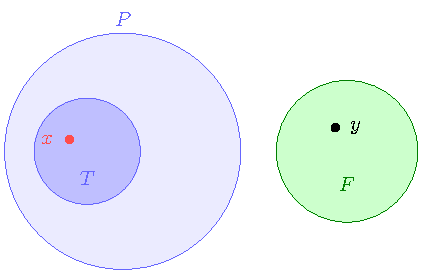
\includegraphics[width=0.9\linewidth]{figures/fig_pertinencia.pdf}

    \caption{Pertinência: $x\in T\subseteq P$ (ponto vermelho dentro de $T$) e $y\in F$ (ponto preto); logo $y\notin P$ e $y\notin T$.}
    \label{fig:pertinencia}\end{figure}


\paragraph{}
Continuando, vem a \textbf{relação de inclusão} entre conjuntos denotada por \(\subseteq\): escrevemos \(X \subseteq Y\) quando todo elemento de \(X\) também pertence a \(Y\) (e \(X\subset Y\) quando, além disso, \(X\neq Y\)). No nosso exemplo, \(A\subseteq T\subset P\) e \(T\cap F=\varnothing\) (árvores e fungos não se sobrepõem).


\begin{figure}[H]
    \centering
    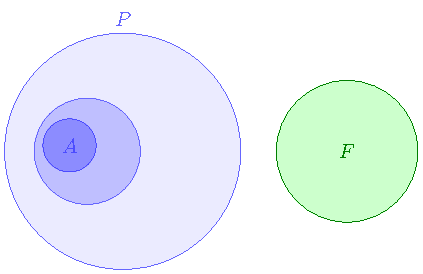
\includegraphics[width=0.9\linewidth]{figures/fig_inclusao.pdf}

    \caption{\texorpdfstring{Inclusão: $A\subseteq T\subset P$ (círculos aninhados) e $T\cap F=\varnothing$ (círculos disjuntos).}{Inclusão: conjuntos aninhados e disjuntos}}
    \label{fig:inclusao}\end{figure}


\subsubsection{Operações entre conjuntos}
\paragraph{}
Com essas definições de pertinência, inclusão e subconjuntos, apresentamos as operações básicas entre conjuntos, que usaremos ao longo do texto (mantendo o exemplo com \(P,T,F,A\)).

Outras operações comuns entre conjuntos incluem:
\begin{itemize}
    \item \textbf{União} (\(A \cup B\)): o conjunto de todos os elementos que pertencem a \(A\), a \(B\), ou ambos.
    
    Exemplo: \(T \cup F\) é o conjunto de todos os organismos que são árvores ou fungos (ou ambos, se existissem tais organismos).
    \begin{figure}[H]
    \centering
    \begin{tikzpicture}[scale=0.95]
        % União T ∪ F com sobreposição visível (intersecção)
        \def\r{1.2}
        \coordinate (LT) at (-0.9,0);
        \coordinate (LF) at (0.9,0);
        % Preenchimento semitransparente para evidenciar a intersecção
        \fill[blue!35, opacity=0.45] (LT) circle (\r);
        \fill[green!35, opacity=0.45] (LF) circle (\r);
        % Contornos e rótulos
        \draw[thick, blue!60] (LT) circle (\r) node[left=6pt] {$T$};
        \draw[thick, green!50!black] (LF) circle (\r) node[right=6pt] {$F$};
    \end{tikzpicture}
    \caption{União: a área colorida representa $T\\cup F$; a sobreposição evidencia a intersecção $T\\cap F$ (hipotética).}
    \label{fig:op-uniao}
    \end{figure}
    
    \paragraph{}
    \item \textbf{União disjunta} (\(A \uplus B\)): o conjunto de todos os elementos que pertencem a \(A\) ou a \(B\), mas não a ambos; é igual a \(A \cup B\) quando \(A\) e \(B\) são disjuntos.
    
    Exemplo: \(T \uplus F\) é o conjunto de todos os organismos que são árvores ou fungos, mas não ambos (o que é trivialmente igual a \(T \cup F\) pois \(T\) e \(F\) são disjuntos).
    \begin{figure}[H]
    \centering
    \begin{tikzpicture}[scale=0.95]
        \def\r{1.1}
        \coordinate (LT) at (-1.8,0);
        \coordinate (LF) at (1.8,0);
        \fill[blue!20] (LT) circle (\r);
        \fill[green!20] (LF) circle (\r);
        \draw[thick, blue!60] (LT) circle (\r) node[left=6pt] {$T$};
        \draw[thick, green!50!black] (LF) circle (\r) node[right=6pt] {$F$};
    \end{tikzpicture}
    \caption{União disjunta: como $T\\cap F=\\varnothing$, tem-se $T\\uplus F = T\\cup F$.}
    \label{fig:op-uniao-disjunta}
    \end{figure}

    \paragraph{}
    \item \textbf{Interseção} (\(A \cap B\)): o conjunto de todos os elementos que pertencem tanto a \(A\) quanto a \(B\).
    
    Exemplo: \(T \cap P = T\), pois todas as árvores são plantas.
    \begin{figure}[H]
    \centering
    \begin{tikzpicture}[scale=0.95]
        % Interseção T ∩ P = T (T ⊆ P)
        \def\rP{1.6}
        \def\rT{0.9}
        \coordinate (cP) at (0,0);
        \coordinate (cT) at (-0.4,0.1);
        % P (maior) e T (dentro de P)
        \draw[fill=blue!10, draw=blue!60, thick] (cP) circle (\rP);
        \node[blue!60] at (0,\rP+0.25) {$P$};
        % Preencher T (interseção equivale a T)
        \draw[fill=blue!35, draw=blue!60, thick] (cT) circle (\rT);
        \node[blue!60] at (cT) {$T$};
    \end{tikzpicture}
    \caption{Interseção: como $T\\subseteq P$, $T\\cap P = T$ (a região escura é $T$).}
    \label{fig:op-intersecao}
    \end{figure}

    \paragraph{}    
    \item \textbf{Diferença} (\(A \setminus B\)): o conjunto de todos os elementos que pertencem a \(A\) mas não a \(B\).
    
    Exemplo: \(T \setminus A\) é o conjunto de todas as árvores que não têm folhas verdes.
    \begin{figure}[H]
    \centering
    \begin{tikzpicture}[scale=0.95]
        % Diferença T \ A (A ⊆ T)
        \def\rT{1.4}
        \def\rA{0.8}
        \coordinate (cT) at (0,0);
        \coordinate (cA) at (0.4,0.2);
        % Preencher T
        \draw[fill=blue!25, draw=blue!60, thick] (cT) circle (\rT);
        % Remover a parte A de dentro de T
        \begin{scope}
            \clip (cT) circle (\rT);
            \fill[white] (cA) circle (\rA);
        \end{scope}
        \draw[thick, blue!60] (cT) circle (\rT) node[above right=2pt and -2pt] {$T$};
        \draw[thick, blue!60] (cA) circle (\rA) node[right=4pt] {$A$};
    \end{tikzpicture}
    \caption{Diferença: região azul representa $T\\setminus A$ (árvores que não têm folhas verdes).}
    \label{fig:op-diferenca}
    \end{figure}
    
    \paragraph{}
    \item \textbf{Complemento} de \(X\) em um universo fixo \(U\): \(X^c := U\setminus X\) (também chamado de \textit{complemento absoluto}); o \textit{complemento relativo} de \(X\) em \(Y\) é \(Y\setminus X\).
    
    Exemplo: \(T^c = U \setminus T\) é o conjunto de todos os organismos que não são árvores. Ou seja, \(T^c\) inclui plantas que não são árvores, fungos e quaisquer outros organismos no universo \(U\).
    \begin{figure}[H]
    \centering
    \begin{tikzpicture}[scale=0.95]
        % Universo U e conjunto T
        \draw[fill=gray!10, draw=black] (-2.6,-1.5) rectangle (2.6,1.5);
        \draw[fill=white, draw=black, thick] (-0.3,0) circle (1.0);
        \node at (-0.3,0) {$T$};
        \node at (2.3,1.25) {$U$};
    \end{tikzpicture}
    \caption{Complemento: a área cinza representa $T^c = U\\setminus T$.}
    \label{fig:op-complemento}
    \end{figure}

    \paragraph{}
    \item \textbf{Diferença simétrica} (\(A\,\Delta\, B\)): \((A\setminus B)\cup(B\setminus A)\); é igual a \(A\cup B\) quando \(A\) e \(B\) são disjuntos.
    
    Exemplo: \(P\,\Delta\, F\) é o conjunto de todos os organismos que são plantas ou fungos, mas não ambos (o que é trivialmente igual a \(P \cup F\) pois \(P\) e \(F\) são disjuntos).
    \begin{figure}[H]
    \centering
    \begin{tikzpicture}[scale=0.95]
        % Diferença simétrica P Δ F com P e F disjuntos
        \def\r{1.2}
        \coordinate (LP) at (-1.6,0);
        \coordinate (LF) at (1.6,0);
        \fill[blue!20] (LP) circle (\r);
        \fill[green!20] (LF) circle (\r);
        \draw[thick, blue!60] (LP) circle (\r) node[left=6pt] {$P$};
        \draw[thick, green!50!black] (LF) circle (\r) node[right=6pt] {$F$};
    \end{tikzpicture}
    \caption{Diferença simétrica: como $P\\cap F=\\varnothing$, temos $P\,\\Delta\, F = P\\cup F$.}
    \label{fig:op-dif-simetrica}
    \end{figure}

    \paragraph{}
    \item \textbf{Produto cartesiano} (\(A\times B\)): o conjunto de pares ordenados \((a,b)\) com \(a\in A\) e \(b\in B\).

    Exemplo: \(T=\{t_1,t_2\}\) e \(F=\{f_1,f_2\}\). Então \(T\times F = \{(t_1,f_1),(t_1,f_2),(t_2,f_1),(t_2,f_2)\}\).
    \begin{figure}[H]
    \centering
    \begin{tikzpicture}[scale=1]
        % Grade limpa para T × F (2×2) sem sobreposições
        \def\xone{0}
        \def\xtwo{2.5}
        \def\yone{0}
        \def\ytwo{1.6}
        % Moldura e linhas da grade
        \draw[gray!35] (\xone-0.4,\yone-0.4) rectangle (\xtwo+0.4,\ytwo+0.4);
        \draw[gray!35] (\xone,\yone) -- (\xone,\ytwo);
        \draw[gray!35] (\xtwo,\yone) -- (\xtwo,\ytwo);
        \draw[gray!35] (\xone,\yone) -- (\xtwo,\yone);
        \draw[gray!35] (\xone,\ytwo) -- (\xtwo,\ytwo);
        % Pontos de T×F com cores distintas por par
        \fill[blue!70] (\xone,\yone) circle (2.4pt);   % (t1,f1)
        \fill[purple!70] (\xone,\ytwo) circle (2.4pt); % (t1,f2)
        \fill[green!60!black] (\xtwo,\yone) circle (2.4pt); % (t2,f1)
        \fill[orange!80!black] (\xtwo,\ytwo) circle (2.4pt); % (t2,f2)
        % Rótulos dos pares (posicionados para não sobrepor)
        \node[font=\scriptsize, text=blue!70, anchor=west]  at (\xone+0.18,\yone+0.18) {$(t_1,f_1)$};
        \node[font=\scriptsize, text=purple!70, anchor=west] at (\xone+0.18,\ytwo) {$(t_1,f_2)$};
        \node[font=\scriptsize, text=green!60!black, anchor=east] at (\xtwo-0.18,\yone+0.18) {$(t_2,f_1)$};
        \node[font=\scriptsize, text=orange!80!black, anchor=east] at (\xtwo-0.18,\ytwo-0.18) {$(t_2,f_2)$};
        % Rótulos dos elementos
        \node[blue!60] at (\xone,\yone-0.45) {$t_1$};
        \node[blue!60] at (\xtwo,\yone-0.45) {$t_2$};
        \node[green!50!black, anchor=east] at (\xone-0.25,\yone) {$f_1$};
        \node[green!50!black, anchor=east] at (\xone-0.25,\ytwo) {$f_2$};
        % Rótulos dos conjuntos (eixos)
        \node at (0.5*\xtwo, -0.95) {$T=\{t_1,t_2\}$};
        \node[rotate=90] at (\xone-0.95, 0.5*\ytwo) {$F=\{f_1,f_2\}$};
    \end{tikzpicture}
    \caption{Produto cartesiano: pontos representam os pares de $T\\times F$ para $T=\{t_1,t_2\}$ e $F=\{f_1,f_2\}$.}
    \label{fig:op-produto}
    \end{figure}

    \paragraph{}
    \item \textbf{Conjunto das partes} (\(2^U\)): a família de todos os subconjuntos de \(U\) (inclui \(\varnothing\) e o próprio \(U\)).
    
    Exemplo: se \(U = \{x,y\}\), então \(2^U = \{\varnothing, \{x\}, \{y\}, \{x,y\}\}\). Logo, \(|2^U|=4=2^{|U|}\).
    \begin{figure}[H]
    \centering
    \begin{tikzpicture}[scale=1, node distance=0.9cm]
        % Diagrama de Hasse para U={x,y}
        \node (empty) at (0,0) {$\varnothing$};
        \node (x) [above left=of empty] {$\{x\}$};
        \node (y) [above right=of empty] {$\{y\}$};
        \node (xy) [above=of empty] {$\{x,y\}$};
        \draw (empty) -- (x) -- (xy) -- (y) -- (empty);
    \end{tikzpicture}
    \caption{Conjunto das partes: diagrama de Hasse de $2^{U}$ para $U=\{x,y\}$.}
    \label{fig:op-partes}
    \end{figure}
\end{itemize}

\paragraph{Identidades úteis.}
Usaremos livremente as propriedades clássicas de conjuntos — comutatividade e associatividade de \(\cup\) e \(\cap\), distributividade e as \textbf{leis de De Morgan} — sem prova. Quando for relevante, explicitaremos a identidade no ponto de uso. Por exemplo, no nosso universo \(U\), \((P\cup F)^c = P^c\cap F^c\).

\subsubsection{Coleção}

\paragraph{}
Entre os objetos que podem pertencer a um conjunto, estão também eles mesmos, outros conjuntos. Chamaremos tais conjuntos de \textbf{coleções} (ou \textbf{famílias}) de conjuntos. Por exemplo, \(\mathcal{C} = \{P, T, F\}\) é uma coleção formada pelos conjuntos de organismos já definidos: plantas \(P\), árvores \(T\) e fungos \(F\). Note que \(\mathcal{C}\) é um conjunto como outro qualquer; seus elementos são, cada um, um conjunto.

\paragraph{}
Coleções são úteis para agrupar subconjuntos relacionados de um mesmo universo. Por exemplo, considere \(\mathcal{D} = \{A, B\}\), onde \(A = \{\text{árvores com folhas verdes}\}\) e \(B = \{\text{árvores com folhas vermelhas}\}\). Assim, \(\mathcal{D} \subseteq 2^{T}\) é uma coleção de subconjuntos de \(T\).

\paragraph{}
Uma coleção \(\mathcal{F}\) é dita \textbf{laminar} quando, para quaisquer \(X, Y \in \mathcal{F}\), vale que \(X \subseteq Y\), \(Y \subseteq X\) ou \(X \cap Y = \varnothing\); isto é, quaisquer dois conjuntos são aninhados (um está contido no outro) ou são disjuntos. 

\paragraph{}
Por exemplo, na coleção \(\mathcal{C} = \{P, T, F\}\): \(P\) é o conjunto de todas as plantas, \(T\) o de todas as árvores (portanto \(T\subseteq P\)) e \(F\) o de todos os fungos (disjunto de plantas e, logo, de árvores). Assim, quaisquer dois conjuntos em \(\mathcal{C}\) são aninhados ou disjuntos, e \(\mathcal{C}\) é laminar. Na coleção \(\mathcal{D} = \{A, T\}\): \(A\) é o conjunto de árvores com folhas verdes e \(T\) o de todas as árvores; como toda árvore de \(A\) é árvore de \(T\), temos \(A\subseteq T\) e a coleção é laminar. Já em \(\mathcal{E} = \{A, R\}\): \(R\) é o conjunto de árvores frutíferas; há árvores que são ao mesmo tempo frutíferas e de folhas verdes (a interseção é não vazia), mas nenhuma das classes contém a outra, então \(\mathcal{E}\) não é laminar.


\begin{figure}[H]
    \centering
    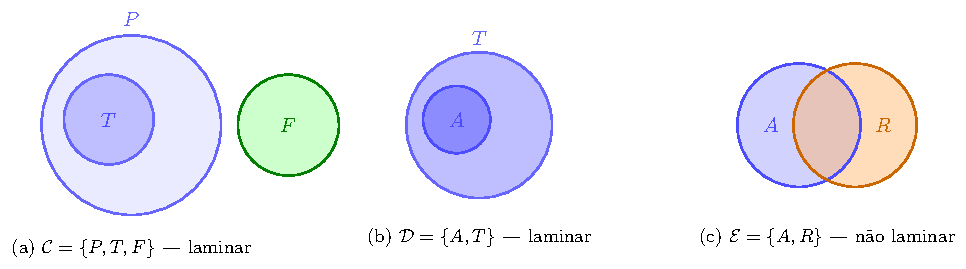
\includegraphics[width=0.9\linewidth]{figures/fig_laminaridade.pdf}

    \caption{Laminaridade em coleções: em (a) e (b), quaisquer dois conjuntos são aninhados ou disjuntos; em (c), $A$ e $R$ se interceptam sem inclusão, violando a laminaridade.}
    \label{fig:laminaridade}\end{figure}


\paragraph{}
Este é um importante conceito que aparecerá no restante do trabalho. A ideia de laminaridade retornará quando tratarmos de cortes dirigidos.

\subsubsection{Comparando conjuntos: cardinalidade e maximalidade}

\paragraph{}
Podemos comparar conjuntos através de relações de tamanho (cardinalidade) ou por relações de inclusão. Essas duas formas de comparação são distintas e importantes, especialmente quando lidamos com coleções de conjuntos.

\paragraph{}
A \textbf{cardinalidade} de um conjunto \(A\), denotada por \(|A|\), é o número de elementos de \(A\). Para conjuntos finitos, é simplesmente a contagem dos elementos (por exemplo, se \(A=\{1,2,3\}\), então \(|A|=3\)). Para conjuntos infinitos, a cardinalidade pode ser mais complexa, envolvendo conceitos como infinito enumerável e não enumerável. Por exemplo, o conjunto dos números naturais \(\mathbb{N}\) é infinito enumerável, enquanto o conjunto dos números reais \(\mathbb{R}\) é infinito não enumerável.

\paragraph{}
Dizemos que \(A\in\mathcal{C}\) tem \textbf{maior cardinalidade} se \(|A|\ge |B|\) para todo \(B\in\mathcal{C}\) (podendo haver empates). Esse critério não coincide, em geral, com a comparação por relação de inclusão. Em grafos, por exemplo, distinguem-se conjuntos independentes \emph{maximais} (não ampliáveis) de conjuntos independentes \emph{máximos} (de cardinalidade máxima).

\paragraph{}
Ao compararmos uma coleção \(\mathcal{C}\) de conjuntos utilizando sua relações de inclusão \((\mathcal{C},\subseteq)\), é imprescindível distinguir \textbf{maximal} de \textbf{máximo}.

\paragraph{}
Um conjunto \(A\in\mathcal{C}\) é \textbf{maximal} se não existe \(B\in\mathcal{C}\) tal que \(A\subset B\). Em palavras: não dá para ampliar \(A\) estritamente dentro da coleção. Podem haver vários elementos maximais, e eles podem ser incomparáveis entre si. Ex.: em \(\mathcal{C}=\big\{\{1\},\{2\}\big\}\), ambos \(\{1\}\) e \(\{2\}\) são maximais, mas não existe máximo.

\paragraph{}
Um conjunto \(A\in\mathcal{C}\) é \textbf{máximo} se \(B\subseteq A\) para todo \(B\in\mathcal{C}\). Se existe, é único. Ex.: em \(\mathcal{C}=\big\{\{1\},\{2\},\{1,2\}\big\}\), o conjunto \(\{1,2\}\) é o máximo.

\paragraph{}
Um bom exemplo para ilustrar a distinção entre conjuntos maximais e máximos é a coleção \(\mathcal{C}=\big\{\{1\},\{2\},\{1,2\},\{3\}\big\}\). Aqui, \(\{1,2\}\) é o único conjunto máximo (contém todos os outros), enquanto \(\{1\}\), \(\{2\}\) e \(\{3\}\) são todos maximais (não podem ser ampliados dentro da coleção).

\paragraph{}
Esses conceitos reaparecerão ao longo do texto, especialmente na diferença entre estruturas \textbf{maximais} (saturadas por inclusão) e \textbf{máximas/ótimas} (de maior cardinalidade ou menor custo). Para fixar ideias:
\begin{itemize}
    \item Em muitos problemas, “\textbf{maximal}” quer dizer: não dá para ampliar uma escolha sem violar as regras; já “\textbf{máximo/ótimo}” quer dizer: entre todas as escolhas válidas, essa é a melhor segundo o critério (por exemplo, menor custo).
    \item No algoritmo de \textbf{Chu--Liu/Edmonds}, começamos com escolhas locais que já não podem ser ampliadas dentro das regras do problema e, a partir delas, chegamos a uma solução de menor custo.
    \item No método de \textbf{András Frank}, primeiro construímos uma estrutura organizada que garante escolhas suficientes; depois, usando apenas relações já ativadas por essa estrutura, extraímos a solução ótima.
    \item Moral: partimos da ideia de “não dá para aumentar” (maximal) e chegamos a “melhor possível” (máximo/ótimo). Os detalhes técnicos de cada método aparecerão nas seções próprias.
\end{itemize}

\subsection{Relações e Funções}

\paragraph{}
Desde a introdução, vimos a ideia filosófica de explicar como “ligar” fatos a hipóteses da forma mais parcimoniosa possível. Para tornar essa intuição precisa, precisamos de uma linguagem que descreva objetos (conjuntos) e como eles se conectam. É aqui que entram as \textbf{relações} e, de modo ainda mais disciplinado, as \textbf{funções}: regras que associam a cada elemento de um conjunto exatamente um elemento de outro. Com elas, passamos do discurso qualitativo sobre explicações para uma estrutura matemática que permite medir, comparar e, adiante, otimizar.

\paragraph{}
Para tornar essa discussão prática, desenvolvemos uma aplicação web interativa que permite visualizar passo a passo o funcionamento dos dois algoritmos, destacando suas diferenças e semelhanças. A seguir, discutimos a dimensão didática que motivou essas escolhas e como fundamentos de aprendizagem e visualização embasam o projeto.

\paragraph{}
Uma \textbf{relação} \(R\) entre dois conjuntos \(A\) e \(B\) é um subconjunto do produto cartesiano \(A \times B\). Ou seja, \(R \subseteq A \times B\). Se \((a,b) \in R\), dizemos que \(a\) está relacionado a \(b\) pela relação \(R\), denotado \(aRb\).


\begin{figure}[H]
    \centering
    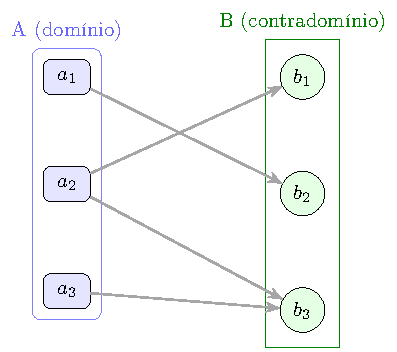
\includegraphics[width=0.9\linewidth]{figures/fig_relacao.pdf}

    \caption{Relação $R\subseteq A\times B$. Cada seta representa um par $(a,b)\in R$ (isto é, $a\,R\,b$). As formas/cores distinguem domínio ($A$, retângulos azuis) de contradomínio ($B$, círculos verdes). Note que $a_2$ se relaciona com $b_1$ e $b_3$; logo, este $R$ \emph{não é função}.}
    \label{fig:relacao}
    \end{figure}


\paragraph{}
No nosso primeiro exemplo-mestre, considere \(P=\{\text{todas as plantas}\}\) e \(F=\{\text{todos os fungos}\}\). Definimos a relação \(R\) como "é um organismo que compete com". Assim, se uma planta \(p \in P\) compete com um fungo \(f \in F\), então \((p,f) \in R\).

\paragraph{}
No nosso segundo exemplo, considere \(H=\{\text{hipóteses}\}\) e \(E=\{\text{evidências}\}\). Definimos a relação \(R\) como "explica". Se uma hipótese \(h \in H\) explica uma evidência \(e \in E\), então \((h,e) \in R\).

\paragraph{}
Em teoria dos grafos, uma relação pode representar conexões entre vértices. Por exemplo, em um grafo dirigido, a relação "existe uma aresta de \(u\) para \(v\)" pode ser representada como um conjunto de pares ordenados \((u,v)\).

\paragraph{}
Uma \textbf{função} \(f\) de um conjunto \(A\) em um conjunto \(B\) é uma relação especial que associa cada elemento de \(A\) a exatamente um elemento de \(B\). Denotamos isso como \(f: A \to B\). Se \(f(a) = b\), dizemos que \(b\) é a imagem de \(a\) sob \(f\).


\begin{figure}[H]
    \centering
    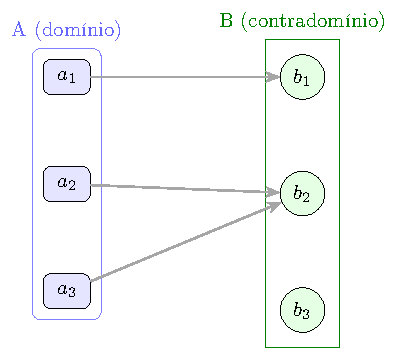
\includegraphics[width=0.9\linewidth]{figures/fig_funcao.pdf}

    \caption{Função $f\!:\!A\to B$. Cada elemento de $A$ tem \emph{exatamente uma} imagem em $B$.}
    \label{fig:funcao}
    \end{figure}


\paragraph{}
No nosso exemplo-mestre, considere \(P=\{\text{todas as plantas}\}\) e \(\mathbb{N}=\{0,1,2,\ldots\}\) (números naturais). Definimos a função \(f: P \to \mathbb{N}\) que associa cada planta ao seu número de folhas. Se \(p \in P\) é uma árvore com 100 folhas, então \(f(p) = 100\).

\paragraph{}
Em teoria dos grafos, funções podem ser usadas para atribuir pesos às arestas. Por exemplo, se temos um grafo \(G\) com arestas \(e_1, e_2, \ldots, e_n\), podemos definir uma função \(c: E \to \mathbb{R}^+\) que atribui um peso \(c(e_i)\) a cada aresta \(e_i\).

\paragraph{}
Na ciência da computação, relações e funções são usadas para modelar conexões entre dados, estruturas de dados e operações. Por exemplo, em bancos de dados relacionais, tabelas representam relações entre diferentes entidades. Em programação funcional, funções são tratadas como cidadãos de primeira classe, permitindo a criação de funções de ordem superior que podem receber outras funções como argumentos ou retorná-las como resultados.

\subsubsection{Conceitos em Funções}
\paragraph{}
Alguns conceitos importantes relacionados a funções incluem:
\begin{itemize}
    \item \textbf{Domínio}: o conjunto \(A\) de entrada da função \(f: A \to B\).
    \item \textbf{Contradomínio}: o conjunto \(B\) de possíveis saídas da função.
    \item \textbf{Imagem}: o conjunto de valores efetivamente atingidos pela função, \(f(A) = \{f(a) \mid a \in A\}\).
    
    \begin{figure}[H]
    \centering
    \begin{tikzpicture}[>=Stealth, node distance=1.1cm]
        % Elementos do domínio A (retângulos azuis)
        \node[draw, rounded corners, fill=blue!10, minimum width=9mm, minimum height=6mm] (a1img) {$a_1$};
        \node[draw, rounded corners, fill=blue!10, below=of a1img, minimum width=9mm, minimum height=6mm] (a2img) {$a_2$};
        \node[draw, rounded corners, fill=blue!10, below=of a2img, minimum width=9mm, minimum height=6mm] (a3img) {$a_3$};
        % Elementos do contradomínio B (círculos verdes)
        \node[circle, draw, fill=green!10, right=3.2cm of a1img, minimum size=6mm] (b1img) {$b_1$};
        \node[circle, draw, fill=green!10, below=of b1img, minimum size=10mm] (b2img) {$b_2$};
        \node[circle, draw, fill=green!10, below=of b2img, minimum size=6mm] (b3img) {$b_3$};
        % Caixas de agrupamento com rótulos
        \node[draw=blue!50, rounded corners, fit=(a1img)(a2img)(a3img), inner sep=5pt, label={[blue!60]above:A (domínio)}] {};
        \node[draw=green!50!black, fit=(b1img)(b2img)(b3img), inner sep=7pt, label={[green!50!black]above:B (contradomínio)}] {};
        % Setas de f (exatamente uma por elemento de A)
        \draw[->, thick, draw=gray!70] (a1img) -- (b1img);
        \draw[->, thick, draw=gray!70] (a2img) -- (b2img);
        \draw[->, thick, draw=gray!70] (a3img) -- (b2img);
        % Destaque da imagem f(A) ⊆ B
    \node[draw=purple!70!black, thick, fit=(b1img)(b2img), inner sep=3pt, label distance=15mm, label={[purple!70!black]right:Imagem $f(A)$}] {};
    \end{tikzpicture}
    \caption{Domínio, contradomínio e imagem: $A$ (retângulos azuis) mapeia via $f$ para $B$ (círculos verdes). A imagem $f(A)$ é o subconjunto de $B$ efetivamente atingido (aqui, $\{b_1,b_2\}$).}
    \label{fig:dom-contradom-imagem}
    \end{figure}
    
    \item \textbf{Injetora}: uma função \(f\) é injetora se \(f(a_1) = f(a_2)\) implica \(a_1 = a_2\); ou seja, elementos distintos do domínio têm imagens distintas.
    \item \textbf{Sobrejetora}: uma função \(f\) é sobrejetora se para todo \(b \in B\), existe \(a \in A\) tal que \(f(a) = b\); ou seja, a imagem é igual ao contradomínio.
    \item \textbf{Bijetora}: uma função que é tanto injetora quanto sobrejetora; estabelece uma correspondência um-para-um entre os elementos de \(A\) e \(B\).
    
\end{itemize}


\begin{figure}[H]
    \centering
    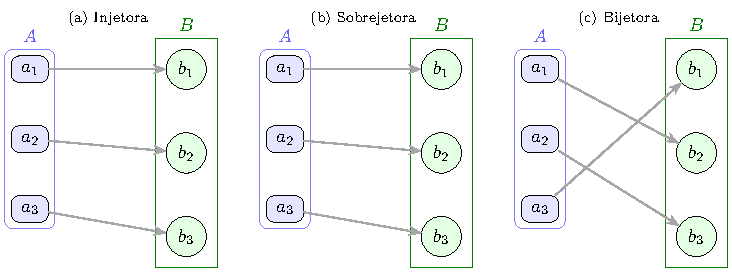
\includegraphics[width=0.9\linewidth]{figures/fig_inj_sobre_bij.pdf}

    \caption{Funções especiais: (a) Injetora — elementos distintos em $A$ têm imagens distintas em $B$; (b) Sobrejetora — todo elemento de $B$ é imagem; (c) Bijetora — um-para-um e sobre $B$.}
    \label{fig:inj-sobre-bij}\end{figure}


\subsubsection{Funções de agregação e somatórios}

\paragraph{}
Além de relacionar elementos de conjuntos, muitas operações familiares em matemática, envolvem \emph{funções} que recebem coleções de números (ou funções) e devolvem um número.

\paragraph{}
Uma \textbf{função de agregação} é uma função que recebe um conjunto (ou sequência) de valores e retorna um único valor que representa algum aspecto agregado desses valores. Exemplos comuns incluem:
\begin{itemize}
    \item \textbf{Média}: A média aritmética de um conjunto de números \(x_1, x_2, \ldots, x_n\) é dada por \(\frac{1}{n}\sum_{i=1}^{n} x_i\).
    \item \textbf{Máximo e Mínimo}: A função máximo retorna o maior valor em um conjunto, enquanto a função mínimo retorna o menor valor.
    \item \textbf{Produto}: O produto de um conjunto de números \(x_1, x_2, \ldots, x_n\) é dado por \(\prod_{i=1}^{n} x_i\).
    \item \textbf{Contagem}: A função contagem retorna o número de elementos em um conjunto.
\end{itemize}

O \textbf{somatório}, por exemplo, é uma função de agregação linear que mapeia uma sequência \((x_1,\dots,x_n)\) em sua soma:
\[\sum_{i=1}^{n} x_i.\]

Esse conceito é especialmente útil em otimização e em análise combinatória: somatórios aparecem o tempo todo e serão explorados ao longo deste trabalho.

\paragraph{Exemplos com grafos.}
As sessões seguintes explorarão em maiores detalhes grafos e dígrafos, mas agora, consideremos a ideia básica: um \textbf{grafo} é um conjunto de pontos (\emph{vértices}) ligados por linhas (\emph{arestas}). No caso \emph{não dirigido}, as linhas não têm seta; no caso \emph{dirigido}, cada linha tem um sentido e é chamada de \emph{arco}.

\paragraph{}
A noção de somatória aparecerá naturalmente quando lidamos com propriedades dos grafos. Por exemplo:

Seja um grafo não dirigido \(G=(V,E)\). O \textbf{grau} de um vértice \(v\in V\), escrito \(\deg(v)\), é quantas arestas tocam em \(v\). A soma dos graus de todos os vértices conta cada aresta \emph{duas vezes} (uma por extremidade), portanto:
\[\sum_{v\in V} \deg(v) = 2\,|E|.\]

Em grafos dirigidos, distinguimos \(\deg^{-}(v)\) (quantos arcos \emph{chegam} em \(v\)) e \(\deg^{+}(v)\) (quantos arcos \emph{saem} de \(v\)). Cada arco contribui com 1 para um grau de saída e 1 para um grau de entrada, logo:
\[\sum_{v\in V} \deg^{-}(v) = \sum_{v\in V} \deg^{+}(v) = |E|.\]

\paragraph{}
Agora suponha que cada aresta/arco \(e\in E\) tenha um \emph{peso} (ou \emph{custo}) \(c(e)\ge 0\). O \textbf{custo total} de um subconjunto \(F\subseteq E\) é simplesmente a soma dos pesos das arestas escolhidas:
\[C(F) = \sum_{e\in F} c(e).\]
De maneira análoga, se \(X\subseteq V\) é um conjunto de vértices, o \textbf{valor total} (ou peso total) dos arcos que \emph{saem} de \(X\) é a soma dos pesos dessas setas. Usaremos mais adiante a notação \(\delta^{+}(X)\) para o conjunto de arcos que saem de \(X\) (ver a seção de dígrafos); com essa notação,
\[\operatorname{val}^+(X) = \sum_{e\in \delta^{+}(X)} c(e).\]
Esses exemplos mostram como somatórios capturam propriedades estruturais do grafo por meio de funções simples de agregação.

\subsubsection{Funções Especiais}

\paragraph{Função de custo}
\paragraph{}Uma \textbf{função de custo} é uma função \(c: A \to \mathbb{R}^+\) que atribui um valor numérico não negativo (custo) a cada elemento de um conjunto \(A\). Essas funções são amplamente utilizadas em otimização, economia e teoria dos grafos para modelar despesas, penalidades ou recursos associados a escolhas ou ações.

\paragraph{}
Exemplo: Considere um conjunto de tarefas \(T = \{t_1, t_2, t_3\}\). Uma função de custo \(c: T \to \mathbb{R}^+\) pode ser definida como:
\[c(t_1) = 5, \quad c(t_2) = 10, \quad c(t_3) = 3.\]
Aqui, \(c(t_i)\) representa o custo de realizar a tarefa \(t_i\). 

\paragraph{}
Depende diretamente do conceito de somatório, pois frequentemente queremos minimizar o custo total de um conjunto de escolhas. Se \(S \subseteq A\) é um subconjunto de elementos escolhidos, o custo total associado a \(S\) é dado por:
\[C(S) = \sum_{a \in S} c(a).\] 

\paragraph{Função c-disjunta}
Uma \textbf{função c-disjunta} é uma função \(f: A \to B\) que, para quaisquer \(a_1, a_2 \in A\) com \(a_1 \neq a_2\), as imagens \(f(a_1)\) e \(f(a_2)\) são disjuntas, ou seja, \(f(a_1) \cap f(a_2) = \varnothing\). Em outras palavras, elementos distintos do domínio são mapeados para conjuntos disjuntos no contradomínio.


\begin{figure}[H]
    \centering
    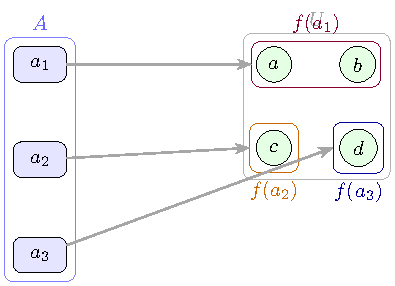
\includegraphics[width=0.9\linewidth]{figures/fig_c_disjunta.pdf}

    \caption{Função c-disjunta: cada \(a\in A\) mapeia para um \emph{subconjunto} de $B$, e imagens de elementos distintos são disjuntas.}
    \label{fig:c-disjunta}
    \end{figure}


\paragraph{}
Exemplo: Considere \(A = \{1, 2, 3\}\) e \(B = \{\{a\}, \{b\}, \{c\}, \{d\}\}\). Definimos a função \(f: A \to B\) como:
\[f(1) = \{a, b\}, \quad f(2) = \{c\}, \quad f(3) = \{d\}.\]
Aqui, \(f\) é c-disjunta, pois \(f(1) \cap f(2) = \varnothing\), \(f(1) \cap f(3) = \varnothing\) e \(f(2) \cap f(3) = \varnothing\).

\paragraph{Função c-viável}

\paragraph{}Uma \textbf{função c-viável} é uma função \(g: A \to \mathbb{R}^+\) que satisfaz certas condições de viabilidade relacionadas a um conjunto de restrições ou critérios. Essas funções são frequentemente usadas em otimização e teoria dos grafos para garantir que as soluções propostas atendam a requisitos específicos.
\paragraph{}
Exemplo: Considere um conjunto de projetos \(P = \{p_1, p_2, p_3\}\) e uma função \(g: P \to \mathbb{R}^+\) que atribui um valor de viabilidade a cada projeto. Suponha que temos a restrição de que a soma dos valores de viabilidade deve ser menor ou igual a um certo limite \(L\). Se definirmos:
\[g(p_1) = 4, \quad g(p_2) = 6, \quad g(p_3) = 3,\]
então a função \(g\) é c-viável se \(g(p_1) + g(p_2) + g(p_3) \leq L\).
\paragraph{}Essas funções são essenciais para garantir que as soluções propostas em problemas de otimização sejam práticas e atendam aos critérios estabelecidos.

\paragraph{Funções de otimização}

\paragraph{}
Do ponto de vista semiótico, “melhor” exprime uma preferência entre interpretações: ao comparar alternativas, escolhemos aquela cuja significação é mais adequada a um critério. Para tornar isso operacional, a matemática troca “fazer mais sentido” por “ter maior (ou menor) valor” em uma escala formal: fixamos (i) um conjunto de soluções viáveis \(\mathcal{F}\) e (ii) uma função numérica sobre \(\mathcal{F}\) que induz uma ordem de comparação.

\paragraph{}
Formalmente, usamos uma \textbf{função objetivo} (ou \textbf{função de otimização})
\[h:\; \mathcal{F} \to \mathbb{R},\]
que atribui um número real a cada solução. Buscamos uma solução \(S^*\in\mathcal{F}\) que \emph{minimize} ou \emph{maximize} \(h\) (isto é, um \(\operatorname*{argmin}\) ou \(\operatorname*{argmax}\)). Quando esse número resulta da soma de contribuições elementares, obtemos o caso aditivo, em ligação direta com os somatórios apresentados antes.

\paragraph{}
Caso \emph{aditivo}. Quando cada elemento \(a\in A\) tem um custo \(c(a)\ge 0\) e as soluções são subconjuntos \(S\subseteq A\), a função objetivo mais comum é o custo total
\[C(S)=\sum_{a\in S} c(a),\]
que desejamos \emph{minimizar}. De modo análogo, se cada item tem um benefício \(p(a)\ge 0\), podemos \emph{maximizar} o benefício total \(P(S)=\sum_{a\in S} p(a)\), possivelmente sujeito a restrições (por exemplo, de orçamento ou limite).

\paragraph{}
Outro exemplo: considere produtos \(X=\{x_1,x_2,x_3\}\) com lucro \(p(x_1)=10\), \(p(x_2)=15\), \(p(x_3)=7\). Se houver um limite de custo que impede escolher todos, o objetivo típico é escolher um subconjunto \(S\subseteq X\) que maximize \(\sum_{x\in S} p(x)\) respeitando as restrições. Essa forma reflete exatamente os somatórios introduzidos antes.

\paragraph{}
Em todos os casos, a função objetivo explicita o critério de “melhor”, e as restrições determinam quais soluções são aceitáveis.

\subsubsection{Otimização}
\paragraph{}
O princípio da navalha de occam nos diz que a explicação mais simples tende a ser a correta. Do ponto de vista semiótico, isso é escolher, entre interpretações possíveis, a que melhor satisfaz um critério. A matemática também se preocupa com identificar a “melhor” solução entre várias alternativas, mas traduz essa ideia em termos quantitativos: fixamos (i) um conjunto de soluções viáveis \(\mathcal{F}\) e (ii) uma função numérica sobre \(\mathcal{F}\) que induz uma ordem de comparação. 

\paragraph{}
Assim, a otimização envolve a maximização ou minimização de uma função objetivo \(h: \mathcal{F} \to \mathbb{R}\) sobre um conjunto de soluções viáveis \(\mathcal{F}\).

\paragraph{}
Esse conceito pode aparecer em muitas necessidades do dia-a-dia: uma empresa pode querer minimizar custos de produção, um viajante pode buscar o caminho mais curto entre dois pontos, ou um investidor pode tentar maximizar o retorno de um portfólio. Em cada caso, a função objetivo quantifica o que significa ser “melhor” ou “mais eficiente”.

\paragraph{}
Pensando em modelagem de problemas em grafos, podemos pensar em exemplos clássicos de otimização:

\begin{itemize}
    \item \textbf{Caminho mais curto}: Dado um grafo com pesos nas arestas, encontrar o caminho entre dois vértices que minimize a soma dos pesos das arestas percorridas.
    \item \textbf{Árvore geradora mínima}: Encontrar uma árvore que conecte todos os vértices de um grafo com o menor custo total das arestas.
    \item \textbf{Fluxo máximo}: Em um grafo direcionado com limites nas arestas, encontrar o fluxo máximo que pode ser enviado de uma fonte a um sumidouro sem exceder esses limites.
\end{itemize}

\subsubsection{A dualidade}

\paragraph{}
O taoísmo chinês fala do yin e yang, forças opostas que se complementam. Um conceito que remete à contrastes, noite e dia, matéria e anti-matéria, máximos e mínimos. Na matemática, um conceito semelhante é a \emph{dualidade}, que conecta problemas de minimização a problemas de maximização.

\paragraph{}
Em termos matemáticos, para cada problema de otimização (o \emph{primal}), existe um problema associado (o \emph{dual}) que oferece uma perspectiva complementar. Resolver um desses problemas pode fornecer insights ou soluções para o outro.

\paragraph{Exemplo:}
Considere um problema de otimização onde queremos minimizar o custo de transporte de mercadorias entre diferentes armazéns. O problema primal busca a solução de transporte que minimize os custos totais, enquanto o problema dual pode ser formulado como a maximização do valor dos recursos disponíveis (como a capacidade dos armazéns e a demanda dos clientes).

\paragraph{}
No nosso texto, consideramos como problema primal a minimização do custo de uma estrutura (como uma árvore geradora mínima) e como dual a maximização de um conjunto de pesos ou preços que justificam esse custo mínimo. A relação entre primal e dual é formalizada por teoremas de dualidade, que garantem que o valor ótimo do primal é igual ao valor ótimo do dual sob certas condições.

\paragraph{}
Esse ponto de vista leva a “teoremas min–max” que ligam problemas de \emph{minimização} a problemas de \emph{maximização} e fornecem certificados verificáveis de otimalidade.


\begin{figure}[H]
    \centering
    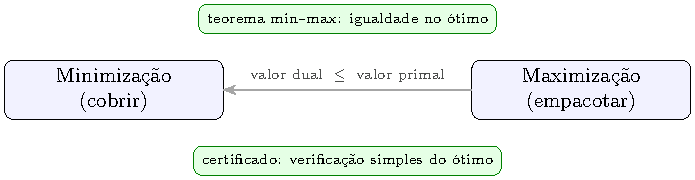
\includegraphics[width=0.9\linewidth]{figures/fig_min_max_cert.pdf}

    \caption{Intuição de min--max: um problema de cobrir (minimização) e um de empacotar (maximização) andam juntos. Sempre vale valor dual $\le$ valor primal; quando há igualdade, temos um certificado de otimalidade.}
    \label{fig:min-max-cert}\end{figure}

\paragraph{}
Uma forma didática de ver a dualidade (no caso linear) é a seguinte. Temos um conjunto de soluções possíveis (um poliedro)
\[P=\{x\in\mathbb{R}^n:\ Ax\ge b\},\]
e um vetor \(c\in\mathbb{R}^n\) que mede o \emph{custo} de cada coordenada de \(x\); o valor da solução é a soma ponderada \(c^\top x\). O problema \textbf{dual} escolhe \(y\ge 0\) (um “preço” para cada restrição de \(Ax\ge b\)) exigindo que nenhuma variável fique “subprecificada”: isso é expresso por
\[A^\top y\ \le\ c.\]
Com essa única condição, todo \(y\ge 0\) fornece automaticamente um \textbf{limitante inferior} para \(c^\top x\) em todo \(P\):
\[c^\top x\ \ge\ (A^\top y)^\top x\ =\ y^\top(Ax)\ \ge\ y^\top b.\]
Geometricamente, \(y^\top b\) é o nível de um \emph{hiperplano de suporte} que nunca ultrapassa a função objetivo \(c^\top x\) sobre \(P\).

No \textbf{ótimo}, existem \(x\) (primal) e \(y\) (dual) viáveis com o \emph{mesmo} valor
\[c^\top x\ =\ y^\top b,\]
isto é, o “vão de dualidade” é zero. Além disso, valem as condições de \textbf{complementaridade}, que dizem “onde há folga de um lado, há zero do outro”:
\[x\odot\big(c-A^\top y\big)=0\quad\text{e}\quad y\odot\big(Ax-b\big)=0.
\]
Interpretando:
\begin{itemize}
    \item Se \(x_j>0\), então o \emph{custo reduzido} daquela coordenada é nulo: \(c_j-(A^\top y)_j=0\). Caso contrário, pode haver folga \(c_j>(A^\top y)_j\) e a variável fica em zero.
    \item Se \(y_i>0\), então a \(i\)-ésima restrição está “apertada” (sem folga): \((Ax-b)_i=0\). Caso contrário, se há folga \((Ax-b)_i>0\), o preço \(y_i\) zera.
\end{itemize}
Essas igualdades capturam a intuição central: o dual estabelece preços que justificam o valor mínimo do primal, e as soluções ótimas usam apenas “direções” cujo custo reduzido é zero e apoiam-se em restrições ativas.

\paragraph{}
No contexto de grafos, a otimização costuma aparecer como a busca por subestruturas (caminhos, árvores, cortes, fluxos) que minimizam ou maximizam um custo, sempre respeitando a topologia do grafo.

\paragraph{}
Nesta dissertação, essa noção de otimização é central: olhamos para o mesmo problema por dois ângulos que se completam. No lado “primal”, queremos montar diretamente a arborescência de menor custo. O algoritmo de Chu–Liu/Edmonds faz isso de forma gulosa: ajusta os custos por vértice, cria arestas de custo zero (0‑arestas), contrai ciclos quando aparecem e segue até montar a solução ótima. 
(\cite{chu1965,edmonds1967optimum}).

\paragraph{}
No lado “dual”, em vez de montar a árvore, colocamos custos em cortes do grafo com raiz $r$. A regra é simples: nenhum custo pode ultrapassar o custo das arestas que cruzam o corte. Buscamos escolher esses custos para somar o máximo possível. As arestas que “batem no limite” viram 0‑arestas, e a partir delas conseguimos reconstruir uma arborescência ótima. Essa visão, desenvolvida por Frank, leva a um teorema min–max e a um procedimento em duas etapas: primeiro ajustamos os custos, depois extraímos a solução usando apenas 0‑arestas. 
(cf. \cite{frank2014,schrijver2003comb})

\subsection{Problemas interessantes}

\paragraph{}
Qual o número mínimo de cores necessárias para colorir um mapa de países, de modo que países vizinhos tenham cores diferentes? Qual o caminho mais curto entre duas cidades em um mapa rodoviário? Como encontrar a árvore geradora mínima que conecta todas as cidades com o menor custo total? Essas perguntas são exemplos clássicos de problemas que podem ser modelados e resolvidos usando a teoria dos grafos. Vistas sob a lente da navalha de occam, todas elas buscam a solução mais parcimoniosa que atende ao requisito: usar poucas cores, percorrer um caminho curto ou conectar tudo com custo mínimo.


\begin{figure}[H]
    \centering
    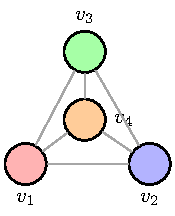
\includegraphics[width=0.9\linewidth]{figures/fig_coloracao.pdf}

    \caption{Coloração de grafos: exemplo de coloração própria do grafo completo $K_4$. Como $K_4$ é completo, precisamos de 4 cores para colorir seus vértices de modo que vértices adjacentes tenham cores diferentes. Uma coloração é uma função $\varphi:V\to C$ tal que, se $uv\in E$, então $\varphi(u)\neq\varphi(v)$.}
    \label{fig:coloracao}\end{figure}


\paragraph{}
Sem a teoria dos grafos, seria difícil formalizar e resolver esses problemas de maneira eficiente. Ao representar situações do mundo real como grafos, tornamos a parcimônia da navalha de occam algo operacional: escolhemos uma medida simples (número de cores, comprimento, custo) e aplicamos algoritmos que, entre as soluções viáveis, minimizam ou maximizam esse critério — produzindo soluções ótimas ou, quando necessário, boas aproximações.

\subsection{Grafos}
\paragraph{}
Falamos bastante de grafos ao longo do texto, aqui fixamos a noção básica. 

\paragraph{}
Um \textbf{grafo} \(G = (V, E)\) é uma estrutura matemática composta por um conjunto \(V\) de \emph{vértices} (ou \emph{nós}) e um conjunto \(E\) de \emph{arestas} (ou \emph{ligações}) que conectam pares de vértices. 


\begin{figure}[H]
    \centering
    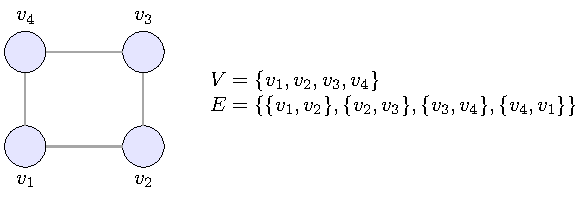
\includegraphics[width=0.9\linewidth]{figures/fig_def_grafo.pdf}

    \caption{Definição de grafo: exemplo de grafo simples \(G=(V,E)\). Pontos representam os vértices \(V\) e linhas representam as arestas \(E\), que são pares não ordenados de vértices distintos.}
    \label{fig:def-grafo}\end{figure}


\paragraph{}
O conjunto de vértices \(V\) pode ser definido como \(V = \{v_1, v_2, \ldots, v_n\}\), onde cada \(v_i\) representa um ponto distinto no grafo. O conjunto de arestas \(E\) é um conjunto de pares não ordenados de vértices, ou seja, \(E \subseteq \{\{u, v\} \mid u, v \in V, u \neq v\}\). Cada aresta \(\{u, v\}\) indica uma conexão entre os vértices \(u\) e \(v\).

\paragraph{}
Esses vértices e arestas podem representar uma variedade de entidades e relações no mundo real. Por exemplo, em um grafo que modela uma rede social, os vértices podem representar pessoas, e as arestas podem representar amizades entre elas. Em um grafo que representa uma rede de transporte, os vértices podem ser cidades, e as arestas podem ser estradas ou rotas de voo conectando essas cidades.

\paragraph{}
Tendo em mente esses problemas, podemos falar de custos associados às arestas. Por exemplo, em um grafo que representa uma rede de transporte, cada aresta pode ter um custo associado, como a distância entre duas cidades ou o tempo necessário para percorrer uma estrada. Em um grafo que modela uma rede de comunicação, as arestas podem ter custos relacionados à largura de banda ou à latência.

\paragraph{}
Esses custos representam uma função \(c: E \to \mathbb{R}^+\) que atribui um valor numérico não negativo a cada aresta do grafo. Assim, para cada aresta \(\{u, v\} \in E\), \(c(\{u, v\})\) representa o custo associado a essa conexão.


\begin{figure}[H]
    \centering
    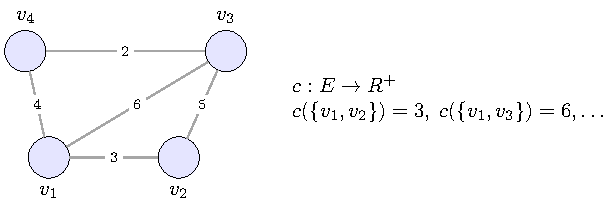
\includegraphics[width=0.9\linewidth]{figures/fig_grafo_custos.pdf}

    \caption{Grafo com custos nas arestas: a função $c:E\to\mathbb{R}^+$ atribui um custo não negativo a cada aresta.}
    \label{fig:grafo-custos}
    \end{figure}


\paragraph{}
Grafos apresentam diversas estruturas especiais. Essas estruturas são definidas como subgrafos e são fundamentais para entender a topologia e as propriedades dos grafos, e muitas vezes são o foco de problemas de otimização. 

\subsubsection{Subgrafos}
\paragraph{}Um \textbf{subgrafo} \(H = (V_H, E_H)\) de um grafo \(G = (V, E)\) é um grafo cujos vértices e arestas são subconjuntos dos vértices e arestas de \(G\). Formalmente, \(V_H \subseteq V\) e \(E_H \subseteq E\), e cada aresta em \(E_H\) conecta dois vértices em \(V_H\).

\paragraph{}
Alguns subgrafos interessantes incluem: caminhos, ciclos, componentes conexas e árvores. Muitas propriedades e algoritmos em grafos dependem dessas estruturas, como encontrar o caminho mais curto entre dois vértices, detectar ciclos ou construir árvores geradoras mínimas. Dentre essas muitas estruturas especiais, vamos apresentar as que são relevantes para o desenvolvimento desta dissertação:

\paragraph{Caminhos}
\paragraph{}Um \textbf{caminho} em um grafo é uma sequência de vértices conectados por arestas. Formalmente, um caminho \(P\) de comprimento \(k\geq 1\) é uma sequência de vértices \(P = (v_1, v_2, \ldots, v_{k+1})\) tal que cada par consecutivo \((v_i, v_{i+1})\) é uma aresta em \(E\). O comprimento do caminho é o número de arestas que ele contém, que é \(k\).


\begin{figure}[H]
    \centering
    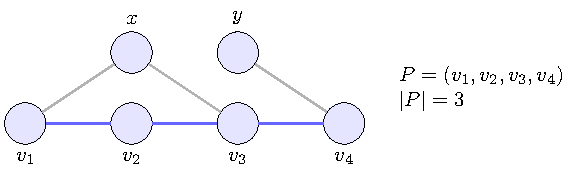
\includegraphics[width=0.9\linewidth]{figures/fig_caminho.pdf}

    \caption{Caminho em grafo não dirigido: o caminho $P=(v_1,v_2,v_3,v_4)$ está destacado em azul. Seu comprimento é o número de arestas percorridas, $|P|=3$.}
    \label{fig:caminho}\end{figure}


\paragraph{Ciclos}
\paragraph{}Um \textbf{ciclo} é um caminho que começa e termina no mesmo vértice, ou seja, \(v_1 = v_{k+1}\). Formalmente, um ciclo \(C\) é uma sequência de vértices \(C = (v_1, v_2, \ldots, v_k, v_1)\) tal que cada par consecutivo \((v_i, v_{i+1})\) é uma aresta em \(E\) e \(k \geq 2\). O comprimento do ciclo é o número de arestas que ele contém, que é \(k\).


\begin{figure}[H]
    \centering
    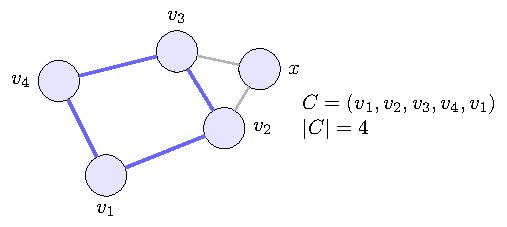
\includegraphics[width=0.9\linewidth]{figures/fig_ciclo.pdf}

    \caption{Ciclo em grafo não dirigido: o ciclo $C=(v_1,v_2,v_3,v_4,v_1)$ está destacado em azul. Seu comprimento é o número de arestas, $|C|=4$.}
    \label{fig:ciclo}\end{figure}


\paragraph{Componentes conexas}
\paragraph{}Uma \textbf{componente conexa} de um grafo é um subgrafo maximal que é conexo. Formalmente, uma componente conexa \(C\) é um subgrafo \(C = (V_C, E_C)\) onde \(V_C \subseteq V\) e \(E_C \subseteq E\), que satisfaz a seguinte propriedade:
\begin{itemize}
    \item \(C\) é conexo: existe um caminho entre qualquer par de vértices em \(V_C\).
\end{itemize}
Além disso, \(C\) é maximal, o que significa que não é possível adicionar mais vértices ou arestas a \(C\) sem perder a propriedade de conexidade.


\begin{figure}[H]
    \centering
    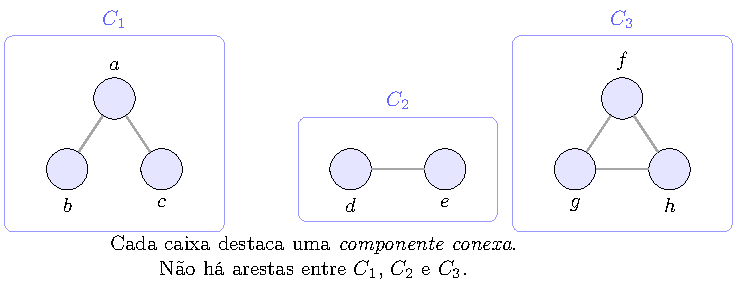
\includegraphics[width=0.9\linewidth]{figures/fig_componentes.pdf}

    \caption{Componentes conexas: o grafo possui três componentes $C_1$, $C_2$ e $C_3$. Cada $C_i$ é conexo e \emph{maximal}, isto é, não pode ser estendido mantendo a conexidade.}
    \label{fig:componentes}
    \end{figure}


\paragraph{Árvores}
\paragraph{}Uma \textbf{árvore} é um grafo conexo e acíclico. Formalmente, uma árvore \(T\) é um grafo \(T = (V_T, E_T)\) onde \(V_T \subseteq V\) e \(E
_T \subseteq E\), que satisfaz as seguintes propriedades:
\begin{itemize}
    \item \(T\) é conexo: existe um caminho entre qualquer par de vértices em \(V_T\).
    \item \(T\) é acíclico: não contém ciclos.
\end{itemize}
Além disso, uma árvore com \(n\) vértices sempre tem exatamente \(n-1\) arestas.


\begin{figure}[H]
    \centering
    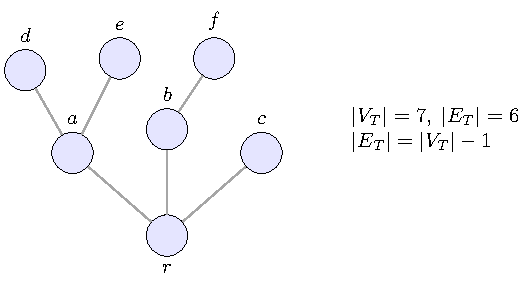
\includegraphics[width=0.9\linewidth]{figures/fig_arvore.pdf}

    \caption{Árvore: grafo conexo e acíclico. No exemplo, $|V_T|=7$ e $|E_T|=6$, satisfazendo $|E_T|=|V_T|-1$. Não há ciclos e existe um único caminho simples entre quaisquer dois vértices.}
    \label{fig:arvore}\end{figure}


\paragraph{}
Para o nosso objetivo principal, nos interessa entendê-las em grafos que a direção das conexões (arestas) importa.

\subsection{Dígrafos: quando a direção importa}
\paragraph{}
Existem problemas que a direção das arestas faz toda a diferença. Por exemplo, em uma rede de tráfego, algumas ruas são de mão única, ou em uma rede de comunicação, os dados podem ser enviados em uma direção específica. Nesses casos, usamos \emph{grafos dirigidos} (ou grafos direcionados ou simplesmente dígrafos), onde as arestas são pares de vértices ordenados.

\paragraph{}
Um \textbf{grafo dirigido - dígrafo} (grafos direcionados) é uma estrutura matemática composta por um conjunto \(V\) de \emph{vértices} e um conjunto \(A\) de \emph{arcos} (ou \emph{arestas direcionadas}) que conectam pares ordenados de vértices.

\paragraph{}
Por vértices entendemos o mesmo conjunto que em grafos comuns, mas agora as arestas entre eles têm uma direção específica. Cada arco \((u, v) \in A\) indica uma conexão direcionada do vértice \(u\) para o vértice \(v\), significando que a relação ou fluxo ocorre de \(u\) para \(v\).

\paragraph{}
Assim, temos os conceitos de cabeça e cauda de um arco: em \((u, v)\), \(u\) é a \emph{cauda} (origem) e \(v\) é a \emph{cabeça} (destino). Esses conceitos podem ser formalizados por meio de funções \(s, t: A \to V\), onde \(s((u, v)) = u\) (cauda) e \(t((u, v)) = v\) (cabeça).


\begin{figure}[H]
    \centering
    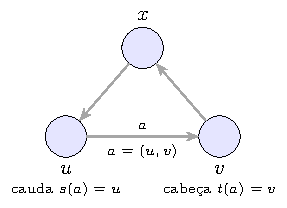
\includegraphics[width=0.9\linewidth]{figures/fig_def_digrafo.pdf}

    \caption{Dígrafos: arcos têm direção. No arco $a=(u,v)$, $u$ é a \emph{cauda} e $v$ é a \emph{cabeça}.}
    \label{fig:def-digrafo}
    \end{figure}


\paragraph{}
Em digrafos podem ocorrer laços (arcos que conectam um vértice a ele mesmo, como \((u, u)\)) nesse caso as funções \(s\) e \(t\) coincidem. Também podem ocorrer múltiplos arcos entre o mesmo par de vértices (como \((u, v)\) e \((u, v)\) distintos). Pictograficamente representamos essas condições com setas com dupla ponta ou com rótulos diferentes.


\begin{figure}[H]
    \centering
    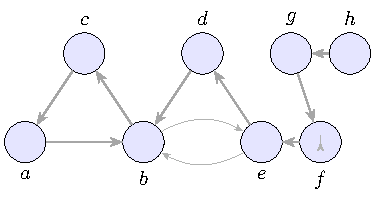
\includegraphics[width=0.9\linewidth]{figures/fig_def_digrafo_simples.pdf}

    \caption{Dígrafo: exemplo de grafo dirigido \(D=(V,A)\). Pontos representam os vértices \(V\) e setas representam os arcos \(A\), que são pares ordenados de vértices. Laços (como \((f,f)\)) e múltiplos arcos (como \((b,e)\) e \((e,b)\)) são permitidos.}
    \label{fig:def-digrafo-simples}\end{figure}
       

\paragraph{}
Tal qual os grafos comuns, os dígrafos podem ter custos associados aos arcos. A função de custo \(c: A \to \mathbb{R}^+\) atribui um valor numérico geralmente não negativo a cada arco do dígrafo. Assim, para cada arco \((u, v) \in A\), \(c((u, v))\) representa o custo associado a essa conexão direcionada.


\begin{figure}[H]
    \centering
    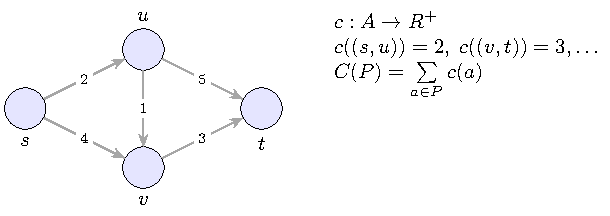
\includegraphics[width=0.9\linewidth]{figures/fig_digrafo_custos.pdf}

    \caption{Dígrafos com custos nos arcos: a função $c:A\to\mathbb{R}^+$ atribui um custo não negativo a cada arco.}
    \label{fig:digrafo-custos}
    \end{figure}


\paragraph{}
Um conceito importante em dígrafos é o de grau de um vértice. O \textbf{grau de entrada} (ou \emph{in-degree}) de um vértice \(v\), denotado por \(d^-(v)\), é o número de arcos que chegam a \(v\) (ou seja, o número de arcos cujo destino é \(v\)). O \textbf{grau de saída} (ou \emph{out-degree}) de um vértice \(v\), denotado por \(d^+(v)\), é o número de arcos que saem de \(v\) (ou seja, o número de arcos cuja origem é \(v\)). Formalmente, temos:
\[d^-(v) = |\{(u, v) \in A \mid u \in V\}|\]
\[d^+(v) = |\{(v, w) \in A \mid w \in V\}|\]

\paragraph{}
Esse conceito é útil para analisar conectividade, o que nos leva ao próximo tópico, empacotamento de vértices.

\paragraph{Empacotamento de Vértices}
\paragraph{}Um \textbf{empacotamento de vértices} (conjunto independente) em um dígrafo é um conjunto \(S\subseteq V\) tal que, no subdígrafo induzido por \(S\), todo vértice tem grau de entrada e de saída iguais a zero. Em notação de graus, se denotamos por \(D[S]\) o subdígrafo induzido, então para todo \(v\in S\) vale \(d^-_{D[S]}(v)=0\) e \(d^+_{D[S]}(v)=0\). Isso é equivalente a dizer que não existe arco com ambas as extremidades em \(S\) (isto é, nenhum \((u,v)\in A\) com \(u,v\in S\)).

\paragraph{Empacotamento Máximo de Vértices}
\paragraph{}
Um \textbf{empacotamento máximo de vértices} é um empacotamento de vértices que contém o maior número possível de vértices. Em outras palavras, é um conjunto \(S\subseteq V\) tal que não existem arcos entre vértices em \(S\) e \(S\) é o maior possível em termos de cardinalidade. Encontrar um empacotamento máximo em um dígrafo é um problema NP-difícil, vamos falar sobre o que isso significa na sessão de algoritmos e complexidade.


\begin{figure}[H]
    \centering
    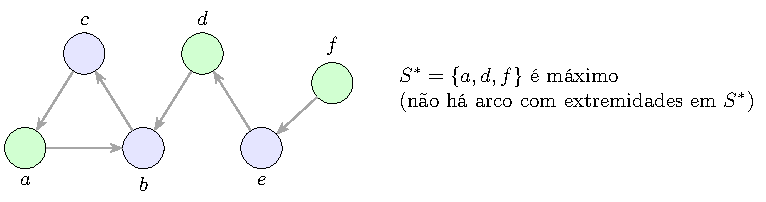
\includegraphics[width=0.9\linewidth]{figures/fig_empacotamento_max.pdf}

    \caption{Empacotamento máximo de vértices: para este dígrafo, $S^{*}$ é um conjunto independente de maior cardinalidade.}
    \label{fig:empacotamento-max}
    \end{figure}


\paragraph{}
Esses conceitos de conectividade e empacotamento de vértices nos levam a explorar as subestruturas especiais que existem em dígrafos, que são similares às que vimos em grafos comuns, mas com algumas diferenças importantes devido à direção dos arcos.

\subsubsection{Subestruturas em dígrafos}

\paragraph{}
Tal qual os grafos que discutimos na sessão anterior, os dígrafos também possuem as mesmas estruturas especiais, essas estruturas chamadas sub-digrafos mudam um pouco em nomenclatura: caminhos quando direcionados são chamados de trilhas, e ciclos são chamados de circuitos e componentes conexas são componentes fortemente conexas e árvores viram arborescências. Além da nomenclatura, a direção dos arcos traz algumas nuances importantes, discutiremos sobre essas nuances apenas na sessão de arborescências e como os algoritmos de busca mudam bastante em complexidade se estamos tratando de arborescências ou árvores comuns.

\paragraph{}
Um \textbf{subdígrafo} \(D' = (V', A')\) de um dígrafo \(D = (V, A)\) é um dígrafo onde \(V' \subseteq V\) e \(A' \subseteq A\). Ou seja, \(D'\) é formado por um subconjunto dos vértices e arcos de \(D\).


\begin{figure}[H]
    \centering
    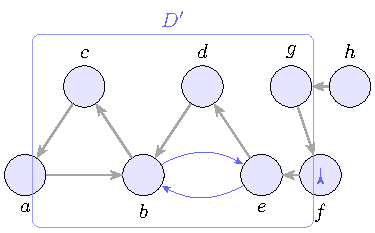
\includegraphics[width=0.9\linewidth]{figures/fig_subdigrafo.pdf}

    \caption{Subdígrafo: o subdígrafo $D'=(V',A')$ está destacado em azul. Aqui, $V'=\{b,c,d,e\}$ e $A'$ contém apenas arcos entre esses vértices.}
    \label{fig:subdigrafo}
    \end{figure}


\paragraph{Subdigrafos Induzidos}
\paragraph{}
Um subdigrafo pode ser \emph{induzido} por um conjunto de vértices \(V' \subseteq V\), denotado como \(D[V']\). Nesse caso, o conjunto de arcos \(A'\) inclui todos os arcos em \(A\) que têm ambas as extremidades em \(V'\), ou seja, \(A' = \{(u, v) \in A \mid u, v \in V'\}\).


\begin{figure}[H]
    \centering
    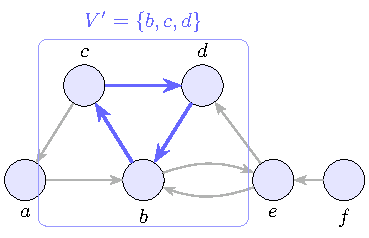
\includegraphics[width=0.9\linewidth]{figures/fig_subdigrafo_induzido.pdf}

    \caption{Subdígrafo induzido: para $V'=\{b,c,d\}$, $D[V']$ mantém todos os arcos com ambas as extremidades em $V'$.}
    \label{fig:subdigrafo-induzido}
    \end{figure}


\paragraph{Subdigrafo Maximal}
\paragraph{}
Um subdigrafo é tido como maximal se não é possível adicionar mais vértices ou arcos a ele sem perder alguma propriedade específica, como conexidade ou aciclicidade.


\begin{figure}[H]
    \centering
    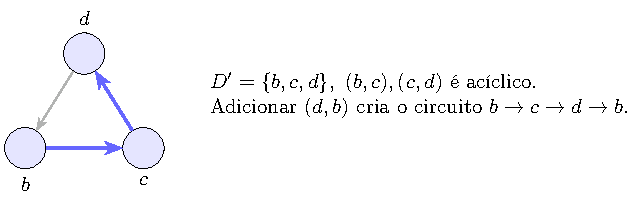
\includegraphics[width=0.9\linewidth]{figures/fig_subdigrafo_maximal.pdf}

    \caption{Subdígrafo maximal (por aciclicidade): $D'$ é acíclico e maximal em $D$; adicionar o arco restante $(d,b)$ cria um circuito.}
    \label{fig:subdigrafo-maximal}\end{figure}


\paragraph{Subdigrafo Gerador}
\paragraph{}
Um subdigrafo é tido como gerador se inclui todos os vértices do dígrafo original, ou seja, \(V' = V\). Nesse caso, o subdigrafo é formado por um subconjunto dos arcos do dígrafo original.


\begin{figure}[H]
    \centering
    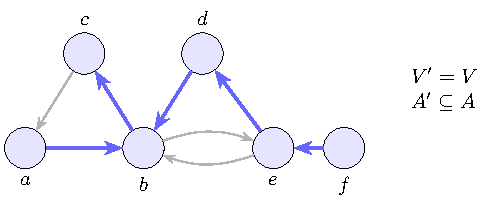
\includegraphics[width=0.9\linewidth]{figures/fig_subdigrafo_gerador.pdf}

    \caption{Subdígrafo gerador: inclui todos os vértices do dígrafo original ($V'=V$) e apenas um subconjunto dos arcos (em azul).}
    \label{fig:subdigrafo-gerador}\end{figure}


\paragraph{}
Com essas definições em mente, podemos explorar as subdigrafos específicos que citaremos ao longo da dissertação, começando pelas trilhas, circuitos, componentes fortemente conexas, componentes-fonte e arborescências.

\subsubsection{Subdigrafos Especiais}

\paragraph{Trilhas}

\paragraph{}
Uma \textbf{trilha} (ou caminho direcionado) em um dígrafo é uma sequência de vértices conectados por arcos que respeitam a direção. Formalmente, uma trilha \(P\) de comprimento \(k \geq 1\) é uma sequência de vértices \(P = (v_1, v_2, \ldots, v_{k+1})\) tal que cada par consecutivo \((v_i, v_{i+1})\) é um arco em \(A\). O comprimento da trilha é o número de arcos que ela contém, que é \(k\).


\begin{figure}[H]
    \centering
    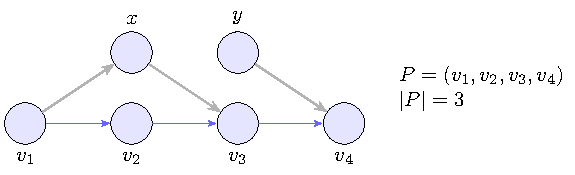
\includegraphics[width=0.9\linewidth]{figures/fig_trilha.pdf}

    \caption{Trilha em dígrafo: a trilha $P=(v_1,v_2,v_3,v_4)$ está destacada em azul. Seu comprimento é o número de arcos percorridos, $|P|=3$.}
    \label{fig:trilha}\end{figure}


\paragraph{}
Uma conceito importante relacionado às trilhas é o de cortes. 

\paragraph{Cortes e Min-cortes}
\paragraph{}
Um \textbf{corte} em um dígrafo é um conjunto de arcos cuja remoção desconecta o dígrafo, ou seja, impede que haja uma trilha entre certos pares de vértices. Formalmente, dado um dígrafo \(D = (V, A)\), um corte \(C\) é um subconjunto de arcos \(C \subseteq A\) tal que a remoção dos arcos em \(C\) resulta em um dígrafo \(D' = (V, A \setminus C)\) onde não existe mais uma trilha (caminho direcionado) entre pelo menos um par de vértices \(u, v \in V\).


\begin{figure}[H]
    \centering
    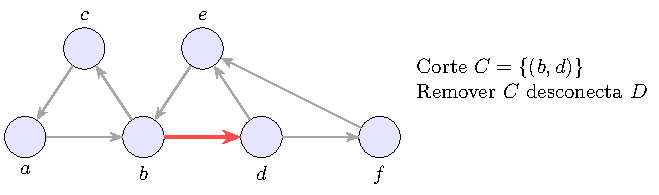
\includegraphics[width=0.9\linewidth]{figures/fig_corte.pdf}

    \caption{Corte em dígrafo: o corte $C=\{(b,d)\}$ remove conectividade de $b$ para $d$.}
    \label{fig:corte}
    \end{figure}


\paragraph{}
De forma resumida, dado um dígrafo \(D=(V,A)\) e um subconjunto \(X\subseteq V\), denotamos por um corte \(s\text{--}t\) é determinado pela escolha de um conjunto de vértices \(X\subseteq V\) tal que \(s\in X\) e \(t\notin X\); pensa-se nele como a “divisão” do grafo em dois lados: \(X\) e \(V\setminus X\).

Para tornar a notação precisa e fácil de ler:
\begin{itemize}
    \item \textbf{\(s\text{--}t\)}: lê-se “de \(s\) para \(t\)”. Aqui, \(s\) é a fonte (onde o fluxo nasce) e \(t\) é o sumidouro (onde o fluxo chega).
    \item \textbf{\(\delta^+(X)\)} (fronteira de saída de \(X\)): conjunto de todos os arcos que \emph{saem} de \(X\) para fora, isto é, para \(V\setminus X\).
    \item \textbf{\(\delta^-(X)\)} (fronteira de entrada de \(X\)): conjunto de todos os arcos que \emph{entram} em \(X\) vindos de \(V\setminus X\). Note que \(\delta^-(X)=\delta^+(V\setminus X)\).
    \item \textbf{Valor do corte}: dado um peso (ou custo) \(c:A\to\mathbb{R}_+\) para cada arco, o valor do corte induzido por \(X\) é a soma dos pesos dos arcos que cruzam de \(X\) para fora: 
    \[c(\delta^+(X))=\sum_{a\in\delta^+(X)} c(a).\]
    No caso não ponderado, esse valor coincide com a \emph{quantidade} de arcos que saem de \(X\).
\end{itemize}

\paragraph{Exemplo:} se \(\delta^+(X)=\{(u_1,v_1),(u_2,v_2)\}\) com \(c((u_1,v_1))=2\) e \(c((u_2,v_2))=3\), então \(c(\delta^+(X))=2+3=5\).

\paragraph{}
Um min-corte é um corte de tamanho mínimo, ou seja, é o corte com o menor número possível de arcos cuja remoção desconecta o dígrafo. Formalmente, dado um dígrafo \(D = (V, A)\), um min-corte \(C_{min}\) é um corte tal que para qualquer outro corte \(C\), \(|C_{min}| \leq |C|\). O tamanho do min-corte é o número de arcos em \(C_{min}\).


\begin{figure}[H]
    \centering
    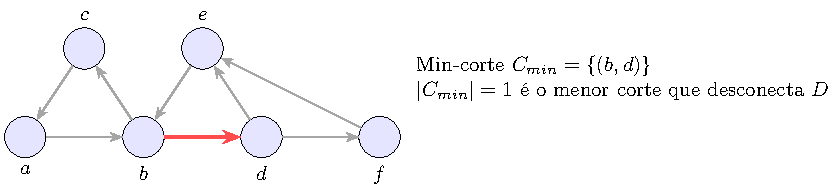
\includegraphics[width=0.9\linewidth]{figures/fig_min_corte.pdf}

    \caption{Min-corte em dígrafo: o min-corte $C_{min}$ é um corte de menor cardinalidade (ou custo) que separa $s$ de $t$.}
    \label{fig:min-corte}
    \end{figure}


Um teorema importante relacionado a min-cortes é o Teorema do Fluxo Máximo - Corte Mínimo, que estabelece uma relação entre o fluxo máximo que pode ser enviado de uma fonte \(s\) para um sumidouro \(t\) em um dígrafo e o valor do min-corte que separa \(s\) de \(t\). Escolhemos apresensentar esse teorema aqui pois ele traz uma intuição interessante sobre a relação entre fluxos e cortes em dígrafos, relevantes para os algoritmos que discutiremos mais adiante.

\paragraph{}
\begin{teobox}{Fluxo–Corte Máximo = Mínimo Corte.}{fluxo-corte}
Em dígrafos com limites/pesos não negativos nos arcos, o valor de um fluxo máximo de \(s\) para \(t\) é igual ao valor de um min-corte \(s\text{--}t\). Em símbolos: \(\max\,\text{valor}(f) = \min\, c(\delta^+(X))\), onde o mínimo é sobre \(X\subseteq V\) com \(s\in X\), \(t\notin X\), e \(c(\delta^+(X))=\sum_{a\in\delta^+(X)} c(a)\).
\paragraph{}
    \textbf{Prova (esboço):}
    \paragraph{}
    \emph{(i) Desigualdade \(\le\).} Seja \(f\) um fluxo qualquer. Para um corte \((X, V\setminus X)\) com \(s\in X\), \(t\notin X\), a conservação de fluxo implica que o fluxo líquido que sai de \(X\) é exatamente \(\text{valor}(f)\).

    Logo, \[\text{valor}(f)= \sum_{a\in\delta^+(X)} f(a) - \sum_{a\in\delta^-(X)} f(a) \le \sum_{a\in\delta^+(X)} f(a) \le \sum_{a\in\delta^+(X)} c(a)=c(\delta^+(X)),\]

    pois \(f(a)\le c(a)\) para todo arco (limite). Como isso vale para todo \(X\), obtemos \(\text{valor}(f)\le \min_X c(\delta^+(X))\).

    \paragraph{}
    \emph{(ii) Desigualdade \(\ge\) e igualdade.} Considere um fluxo máximo \(f\) sem caminho aumentante no \emph{grafo residual} \(R_f\) (isto é, não há como aumentar o valor do fluxo). Defina \(X\) como o conjunto de vértices alcançáveis a partir de \(s\) em \(R_f\). Então, não existe arco residual de \(X\) para \(V\setminus X\); logo, todo arco original que sai de \(X\) está saturado (\(f(a)=c(a)\)), e todo arco que entra em \(X\) carrega fluxo zero. Assim,

    \[\text{valor}(f)=\sum_{a\in\delta^+(X)} f(a)=\sum_{a\in\delta^+(X)} c(a)=c(\delta^+(X)).\]
    Portanto, \(f\) atinge exatamente o valor de um corte \(s\text{--}t\); em particular, esse corte é mínimo e \(f\) é máximo. \hfill$\square$

\paragraph{}
\smallskip
\textbf{Comentário:} Esse resultado é um protótipo de teorema \emph{min--max}: “empacotar” muito fluxo (caminhos) equivale a “cobrir” pouco com um corte. Ver, por exemplo, \cite{schrijver2003comb}.
\end{teobox}

\paragraph{}
Quando falamos em trilhas, precisamos também falar sobre circuitos, que são ciclos direcionados.
A diferença entre trilhas e circuitos é que trilhas são caminhos direcionados que não necessariamente retornam ao ponto de origem, enquanto circuitos são caminhos direcionados que começam e terminam no mesmo vértice.

\paragraph{Circuitos}
\paragraph{}
 Um \textbf{circuito} é um caminho direcionado que começa e termina no mesmo vértice, ou seja, \(v_1 = v_{k+1}\). Formalmente, um circuito \(C\) é uma sequência de vértices \(C = (v_1, v_2, \ldots, v_k, v_1)\) tal que cada par consecutivo \((v_i, v_{i+1})\) é um arco em \(A\) e \(k \geq 2\). O comprimento do circuito é o número de arcos que ele contém, que é \(k\).


\begin{figure}[H]
    \centering
    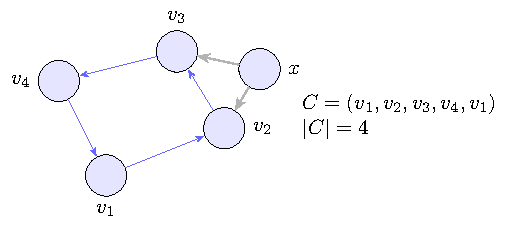
\includegraphics[width=0.9\linewidth]{figures/fig_ciclo_direcionado.pdf}

    \caption{Ciclo direcionado em dígrafo: o ciclo $C=(v_1,v_2,v_3,v_4,v_1)$ está destacado em azul. Seu comprimento é o número de arcos, $|C|=4$.}
    \label{fig:ciclo-direcionado}\end{figure}


\paragraph{}
Propriedades importantes dos circuitos incluem:
\begin{itemize}
    \item \textbf{Circuito simples}: um circuito é dito simples se não repete vértices, exceto o vértice inicial/final. Ou seja, \(v_i \neq v_j\) para \(1 \leq i < j \leq k\).
    \item \textbf{Circuito Euleriano}: um circuito que percorre cada arco exatamente uma vez. Um dígrafo possui um circuito euleriano se e somente se é fortemente conexo e o grau de entrada é igual ao grau de saída para cada vértice.
    \item \textbf{Circuito Hamiltoniano}: um circuito que visita cada vértice exatamente uma vez, exceto o vértice inicial/final. Determinar a existência de um circuito hamiltoniano é um problema que chamamos de NP-completo. Vamos explicar mais sobre isso na seção de algoritmos e complexidade computacional.
\end{itemize}       

\paragraph{}
Existe um princípio chamado de princípio da casa dos pombos, que diz que se você tem mais pombos do que casas, pelo menos uma casa deve conter mais de um pombo. Em termos de grafos, isso se traduz na ideia de que se um grafo tem mais arestas do que vértices, ele deve conter pelo menos um ciclo.

\paragraph{}
Esse princípio também se aplica a dígrafos, mas com uma nuance importante: em dígrafos, o critério correto para garantir a existência de um circuito dirigido é que o grau mínimo de saída (ou de entrada) seja pelo menos 1. Ou seja, se cada vértice em um dígrafo tem pelo menos um arco saindo dele (ou entrando nele), então o dígrafo deve conter pelo menos um circuito dirigido. Abaixo apresentamos esse resultado formalmente.

\paragraph{}
\begin{lemabox}{Princípio da casa dos pombos para circuitos.}{casa-dos-pombos}
Se \(D=(V,A)\) é um dígrafo finito em que todo vértice tem grau de saída ao menos 1, isto é, \(d^+(v)\ge 1\) para todo \(v\in V\), então \(D\) contém pelo menos um circuito dirigido. (De forma equivalente, a afirmação vale trocando ``saída'' por ``entrada''.)

\paragraph{}
	\textbf{Prova:} Escolha para cada \(v\in V\) um arco \((v,f(v))\) que sai de \(v\) (possível porque \(d^+(v)\ge 1\)). Fixa\-do um vértice \(v_0\), considere a sequência \(v_0, v_1=f(v_0), v_2=f(v_1),\dots\). Como \(V\) é finito, algum vértice repete: existem \(i<j\) com \(v_i=v_j\). O trecho \(v_i\to v_{i+1}\to\cdots\to v_j=v_i\) é um circuito dirigido em \(D\). A versão com graus de entrada segue aplicando o argumento ao dígrafo com arcos invertidos. \hfill$\square$

\paragraph{}
\smallskip
	\textbf{Observação:} A condição \(|A|>|V|\) \emph{não} garante a existência de circuito dirigido em geral (há orientações acíclicas com muitos arcos). O critério correto, simples e útil, é o grau mínimo de saída (ou de entrada) ser pelo menos 1. Ver, por exemplo, \cite{schrijver2003comb}.

\end{lemabox}

\paragraph{}
Esse princípio ajuda a entender o comportamento básico dos métodos que os algoritmos empregam para encontrar as arborescências de custo mínimo. Vamos elaborar melhor esse ponto na seção de algoritmos em arborescências, especialmente ao discutir o algoritmo de Chu--Liu/Edmonds.

\paragraph{}
No algoritmo de Chu--Liu/Edmonds que exploraremos em detalhes em capítulo posterior, para cada vértice \(v\neq r\), escolhemos a aresta de menor custo que entra em \(v\), o subgrafo obtido fica com grau de entrada igual a 1 em todos os \(v\neq r\). Pelo lema, enquanto esse subgrafo ainda não for uma arborescência, ele necessariamente contém um circuito: assim o algoritmo se baseia em detectar o circuitos, contraí-lo a um único vértice e repetir a seleção sob custos reduzidos. Quando não houver mais circuitos, as arestas escolhidas formam uma arborescência ótima enraizada em \(r\).

\paragraph{Componentes fortemente conexas}
\paragraph{}Uma \textbf{componente fortemente conexa} (abreviaremos como \textbf{CFC}) é um subdígrafo maximal onde existe um caminho direcionado (trilha) entre qualquer par de vértices. 

\paragraph{}
Formalmente, uma componente fortemente conexa \(C\) é um subdígrafo \(C = (V_C, A_C)\) onde \(V_C \subseteq V\) e \(A_C \subseteq A\), que satisfaz a seguinte propriedade:
\begin{itemize}
    \item \(C\) é fortemente conexo: existe um caminho direcionado entre qualquer par de vértices em \(V_C\).
\end{itemize}
Além disso, \(C\) é maximal, o que significa que não é possível adicionar mais vértices ou arcos a \(C\) sem perder a propriedade de forte conexidade.

\begin{figure}[H]
    \centering
    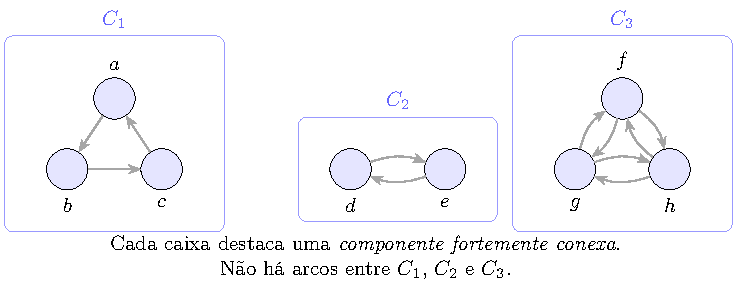
\includegraphics[width=0.9\linewidth]{figures/figure_028.pdf}

    \caption{Componentes fortemente conexas: o dígrafo possui três componentes $C_1$, $C_2$ e $C_3$. Cada $C_i$ é fortemente conexo e \emph{maximal}.}
    \end{figure}


\paragraph{}
A seguir falaremos sobre a propriedade de alcançabilidade mútua em CFC, que é fundamental para entendermos a relação entre elas e arborescências (que apenas mencionaremos aqui, para aprofundarmos na sessão sobre arborescências e com os grafos acíclicos dirigidos (DAGs))\footnote{Um DAG (Directed Acyclic Graph) é um grafo direcionado que não contém ciclos. Em outras palavras, não é possível começar em um vértice e seguir uma sequência de arcos que retorne ao mesmo vértice. Os DAGs são estruturas fundamentais em muitas áreas da computação, incluindo a representação de dependências e a modelagem de processos.}:

\begin{itemize}
    \item \textbf{CFCs e alcançabilidade mútua:} dois vértices \(u\) e \(v\) pertencem à mesma CFC se, e somente se, \(u\leadsto v\) e \(v\leadsto u\). Ou seja, existe um caminho direcionado de \(u\) para \(v\) e um caminho direcionado de \(v\) para \(u\). A relação de pertencer à mesma CFC é uma relação de equivalência que particiona o conjunto de vértices \(V\) em subconjuntos disjuntos, cada um correspondendo a uma CFC.
    \item \textbf{Arborescências em dígrafos fortemente conexos:} um dígrafo é fortemente conexo se, e somente se, para algum (equiv., para todo) vértice $r$ existem uma \emph{arborescência de saída} enraizada em $r$ que alcança todos os vértices e uma \emph{arborescência de entrada} enraizada em $r$ que é alcançada por todos os vértices. De fato, se $D$ é fortemente conexo, basta rodar buscas a partir de $r$; no sentido inverso, $r\leadsto v$ pela arborescência de saída e $v\leadsto r$ pela de entrada, implicando alcançabilidade mútua entre quaisquer dois vértices via $r$.
    \item \textbf{CFC e DAG.} Ao \emph{contrair} cada CFC a um único vértice obtemos o grafo condensado $\mathrm{Cond}(D)$\footnote{O grafo condensado é uma representação simplificada do dígrafo original, onde as CFCs são representadas como vértices únicos.}. Não há circuitos dirigidos em $\mathrm{Cond}(D)$; portanto, ele é um DAG.
    
    \paragraph{Consequências:}
     todo DAG tem ao menos uma componente-fonte (falaremos em seguida sobre eles) e uma componente-sumidouro; logo, $\mathrm{Cond}(D)$ também tem ao menos uma CFC-fonte e ao menos uma CFC-sumidouro.
\end{itemize}

\paragraph{Componentes-fonte}
\paragraph{}Uma \textbf{componente-fonte} é uma componente fortemente conexa que não possui arcos direcionados saindo dela para outras componentes. Formalmente, uma componente-fonte \(C\) é uma componente fortemente conexa \(C = (V_C, A_C)\) onde \(V_C \subseteq V\) e \(A_C \subseteq A\), que satisfaz a seguinte propriedade:
\begin{itemize}
    \item Não existem arcos \((u, v) \in A\) tais que \(u \in V_C\) e \(v \notin V_C\).
    \item \(C\) é maximal: não é possível adicionar mais vértices ou arcos a \(C\) sem perder a propriedade de forte conexidade.
    \item \(C\) é fortemente conexo: existe um caminho direcionado entre qualquer par de vértices em \(V_C\).
\end{itemize}


\begin{figure}[H]
    \centering
    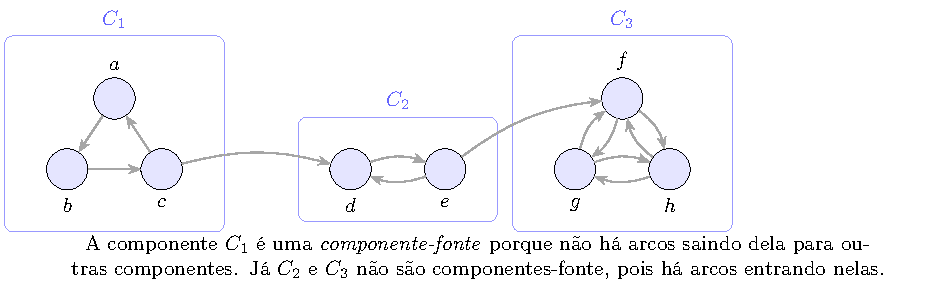
\includegraphics[width=0.9\linewidth]{figures/fig_componente_fonte.pdf}

    \caption{Componente-fonte: o dígrafo possui três componentes $C_1$, $C_2$ e $C_3$. A componente $C_1$ é uma componente-fonte porque não há arcos saindo dela para outras componentes. Já $C_2$ e $C_3$ não são componentes-fonte, pois há ar  cos entrando nelas.}
    \label{fig:componente-fonte}\end{figure}


\paragraph{Componentes-sumidouro}
\paragraph{}Uma \textbf{componente-sumidouro} é uma componente fortemente conexa que não possui arcos direcionados entrando nela vindos de outras componentes. Formalmente, uma componente-sumidouro \(C\) é uma componente fortemente conexa \(C = (V_C, A_C)\) onde \(V_C \subseteq V\) e \(A_C \subseteq A\), que satisfaz a seguinte propriedade:
\begin{itemize}
    \item Não existem arcos \((u, v) \in A\) tais que \(u \notin V_C\) e \(v \in V_C\).
    \item \(C\) é maximal: não é possível adicionar mais vértices ou arcos a \(C\) sem perder a propriedade de forte conexidade.
    \item \(C\) é fortemente conexo: existe um caminho direcionado entre qualquer par de vértices em \(V_C\).
\end{itemize}


\begin{figure}[H]
    \centering
    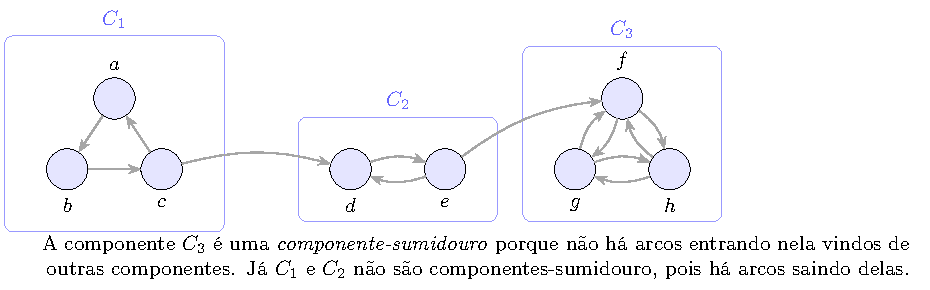
\includegraphics[width=0.9\linewidth]{figures/fig_componente_sumidouro.pdf}

    \caption{Componente-sumidouro: o dígrafo possui três componentes $C_1$, $C_2$ e $C_3$. A componente $C_3$ é uma componente-sumidouro porque não há arcos entrando nela vindos de outras componentes. Já $C_1$ e $C_2$ não são componentes-sumidouro, pois há arcos saindo delas.}
    \label{fig:componente-sumidouro}\end{figure}


\paragraph{}
Existe um resultado clássico que relaciona o número de componentes-fonte e componentes-sumidouro em um dígrafo com o número mínimo de arcos necessários para torná-lo fortemente conexo.


\begin{figure}[H]
    \centering
    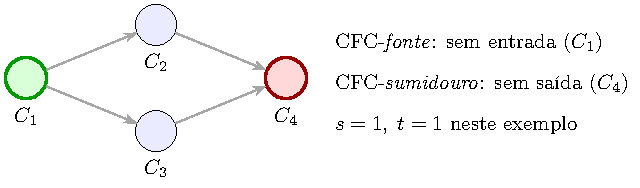
\includegraphics[width=0.9\linewidth]{figures/fig_condensado_st.pdf}

    \caption{Grafo condensado $\mathrm{Cond}(D)$: cada CFC é contraída a um vértice e não há circuitos dirigidos (DAG).}
    \label{fig:condensado-st}
    \end{figure}


\paragraph{}
Seja $D=(V,A)$ um dígrafo com $k$ componentes fortemente conexas (CFCs): 

\paragraph{}
Denote por $\mathrm{Cond}(D)$ o grafo \emph{condensado}, obtido ao contrair cada CFC de $D$ em um único vértice; $\mathrm{Cond}(D)$ é sempre um DAG. Escreva $s$ para o número de CFCs-\emph{fonte} (vértices de $\mathrm{Cond}(D)$ sem arcos de \emph{entrada}) e $t$ para o número de CFCs-\emph{sumidouro} (vértices de $\mathrm{Cond}(D)$ sem arcos de \emph{saída}). Com essa notação, vale o seguinte:

\paragraph{}
\begin{lemabox}{Mínimo de arcos para conexidade forte}{min-arc}
Se $k=1$, então $D$ já é fortemente conexo e o mínimo de arcos a adicionar é $0$. Se $k\ge 2$, o número mínimo de arcos a adicionar para tornar $D$ fortemente conexo é \[\boxed{\;\min = \max\{s,\,t\}\;}\,.\]

\paragraph{}
	\textbf{Prova (esboço).} 
    \paragraph{}
    \emph{Necessidade:} em qualquer supergrafo fortemente conexo, cada CFC-fonte deve receber ao menos um arco \emph{entrando} e cada CFC-sumidouro deve ter ao menos um arco \emph{saindo}; logo, são necessários ao menos $\max\{s,t\}$ arcos novos. 
    
    \paragraph{}
    \emph{Suficiência:} numa ordenação topológica de $\mathrm{Cond}(D)$, conecte CFCs-sumidouro a CFCs-fonte de modo a formar um ciclo que percorra todas as CFCs. Isso pode ser feito com exatamente $\max\{s,t\}$ arcos, mesmo quando $s\ne t$, emparelhando sobras de um lado com o outro. 
    
    \paragraph{}
    Ver, por exemplo, textos clássicos sobre dígrafos (e.g., \cite{schrijver2003comb}).
\end{lemabox}

\paragraph{}
Esse lema explica por que todo dígrafo com mais de uma CFC-fonte ou mais de uma CFC-sumidouro não pode ser fortemente conexo. Além disso, ele é útil em algoritmos que buscam tornar um dígrafo fortemente conexo, pois fornece um limite inferior para o número de arcos que precisam ser adicionados.

\paragraph{}
As noções de CFCs e componentes-fonte conversam diretamente com o conceito de \emph{arborescências}. Pois, em uma arborescência, todos os vértices são alcançáveis a partir da raiz, o que não implica que a arborescência é fortemente conexa, mas encontrar essas componentes dentro de um dígrafo pode nos ajudar em uma busca otimizada por arborescências.

\paragraph{Arborescências}

\paragraph{}Uma \textbf{arborescência} é um dígrafo acíclico e conexo, onde há um vértice especial chamado \emph{raiz} que tem um caminho direcionado para todos os outros vértices. Formalmente, uma arborescência \(T\) é um dígrafo \(T = (V_T, A_T)\) onde \(V_T \subseteq V\) e \(A_T \subseteq A\), que satisfaz as seguintes propriedades:
\begin{itemize}
    \item \(T\) é conexo: existe um caminho direcionado da raiz para qualquer vértice em \(V_T\).
    \item \(T\) é acíclico: não contém ciclos direcionados.
\end{itemize}
Além disso, uma arborescência com \(n\) vértices sempre tem exatamente \(n-1\) arcos.

\begin{figure}[H]
    \centering
    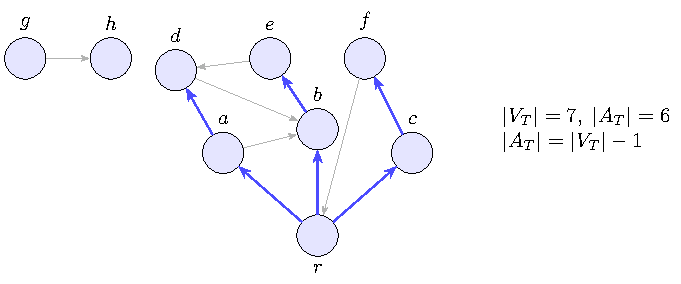
\includegraphics[width=0.9\linewidth]{figures/fig_arborescencia.pdf}

    \caption{Arborescência: dígrafo conexo e acíclico com raiz $r$ de onde há um caminho direcionado para todos os outros vértices em azul. No exemplo, $|V_T|=7$ e $|A_T|=6$, satisfazendo $|A_T|=|V_T|-1$. Em cinza, arcos que não fazem parte da arborescência.}
    \label{fig:arborescencia}\end{figure}


\paragraph{Definições e notação adicionais}
\paragraph{}
Para facilitar a discussão sobre arborescências, introduzimos algumas definições e notações adicionais: seja \(D = (V, A)\) um dígrafo e \(r \in V\) um vértice específico (a raiz). Denotamos por \(d_D^+(v)\) o grau de saída de um vértice \(v\) em \(D\), ou seja, o número de arcos que saem de \(v\). Analogamente, \(d_D^-(v)\) é o grau de entrada de \(v\), o número de arcos que entram em \(v\).


\paragraph{}
As arborescências são o principal objeto de investigação desse trabalho, portanto vamos usar uma sessão dedicada a elas para apresentar suas características, variações e aplicações.

\subsection{Arborescências em foco}

\paragraph{}
Já tratamos do conceito básico de arborescência, agora falaremos de arborescências especiais:

\paragraph{Arborescência Geradora:}
Uma arborescência é considerada geradora se inclui todos os vértices do dígrafo original, ou seja, \(V_T = V\). Nesse caso, a arborescência é formada por um subconjunto dos arcos do dígrafo original.

\paragraph{Arborescência Maximal:}
Uma arborescência é dita maximal se não é possível adicionar mais vértices ou arcos a ela sem perder a propriedade de ser uma arborescência, ou seja, sem criar ciclos ou desconectar o dígrafo.

\paragraph{Ramificações Geradoras}
\paragraph{}Uma \textbf{ramificação geradora} é um subdígrafo que é uma arborescência que inclui todos os vértices do dígrafo original. Formalmente, uma ramificação geradora \(R\) é um subdígrafo \(R = (V_R, A_R)\) onde \(V_R = V\) e \(A_R \subseteq A\), que satisfaz as seguintes propriedades:
\begin{itemize}
    \item \(R\) é uma arborescência: existe um vértice especial chamado raiz que tem um caminho direcionado para todos os outros vértices.
    \item \(R\) é maximal: não é possível adicionar mais arcos a \(R\) sem perder a propriedade de ser uma arborescência.
\end{itemize}


\begin{figure}[H]
    \centering
    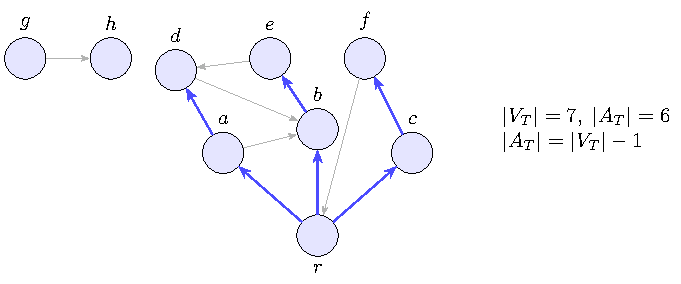
\includegraphics[width=0.9\linewidth]{figures/fig_ramificacao_geradora.pdf}

    \caption{Ramificação geradora: arborescência que inclui todos os vértices do dígrafo original, em azul. No exemplo, $|V_T|=7$ e $|A_T|=6$, satisfazendo $|A_T|=|V_T|-1$. Em cinza, arcos que não fazem parte da ramificação geradora.}
    \label{fig:ramificacao-geradora}\end{figure}
 

\paragraph{}
Quando falamaos de ramificações geradoras, podemos falar de uma estrutura que fixa um vértice raiz \(r\) e constrói uma arborescência que alcança todos os outros vértices a partir dessa raiz. Essa estrutura é conhecida como \emph{r-arborescência}.

\paragraph{Arborescência de Raiz Específica:}
uma arborescência de raiz específica é uma arborescência onde a raiz é um vértice pré-determinado do dígrafo. Isso é útil em situações onde um ponto de origem específico deve ser o início dos caminhos direcionados para todos os outros vértices. Podemos chamá-la de r-arborescência, onde \(r\) é o vértice raiz.

\paragraph{}
Em uma arborescência \(T = (V_T, A_T)\) enraizada em \(r\), temos as seguintes propriedades:
\begin{itemize}
    \item A raiz \(r\) tem grau de entrada zero: \(d_T^-(r) = 0\).
    \item Todo outro vértice \(v \in V_T \setminus \{r\}\) tem grau de entrada exatamente um: \(d_T^-(v) = 1\). Isso significa que há exatamente um arco direcionado entrando em cada vértice, exceto na raiz.
    \item O grau de saída \(d_T^+(v)\) pode variar, mas para garantir que \(T\) seja conexo, deve haver pelo menos um arco saindo de \(r\) para alcançar os outros vértices.
\end{itemize}

\paragraph{Arborescência inversa (in-arborescência):}
uma \emph{arborescência inversa} enraizada em \(r\) — também chamada de \emph{in-arborescência} — é o resultado de inverter a orientação de todos os arcos de uma arborescência (out-arborescência) enraizada em \(r\). Equivalentemente: é um dígrafo acíclico no qual, para todo \(v\neq r\), existe \emph{exatamente um} caminho direcionado de \(v\) até \(r\) (isto é, todos os arcos estão orientados \emph{em direção} à raiz). Em termos de graus, numa in-arborescência cada vértice \(v\neq r\) tem grau de saída igual a 1 (o arco para seu “pai”) e a raiz \(r\) tem grau de saída 0; os graus de entrada são complementares aos de uma out-arborescência.

\paragraph{}
As arborecências podem ter custos associados aos seus arcos, o que nos leva ao conceito de arborescência de custo mínimo.

\paragraph{Arborescência de Custo Mínimo:}
\paragraph{}
Uma \textbf{arborescência de custo mínimo} é uma arborescência que minimiza a soma dos pesos dos arcos que a compõem. Esse conceito é especialmente relevante em aplicações onde os arcos têm custos associados, como em redes de transporte ou comunicação.

\paragraph{}
Finalmente podemos conceituar a principal estrutura que estudaremos nesta dissertação: a r-arborescência de custo mínimo e sua variante, a r-arborescência inversa de custo mínimo.

\paragraph{r-arborescência de custo mínimo:}
é uma arborescência enraizada em um vértice específico \(r\) que minimiza a soma dos pesos dos arcos que a compõem. Formalmente, dada uma função de custo \(c: A \to \mathbb{R}_{\geq 0}\) que atribui um custo a cada arco do dígrafo \(D = (V, A)\), uma r-arborescência de custo mínimo \(T\) é uma arborescência \(T = (V_T, A_T)\) onde \(V_T \subseteq V\) e \(A_T \subseteq A\), que satisfaz as seguintes propriedades:
\begin{itemize}
    \item \(T\) é uma arborescência enraizada em \(r\): existe um caminho direcionado de \(r\) para qualquer vértice em \(V_T\).
    \item \(T\) minimiza o custo total: a soma dos custos dos arcos em \(A_T\) é mínima, ou seja, \(\sum_{a \in A_T} c(a)\) é minimizada.
\end{itemize}

\begin{figure}[H]
    \centering
    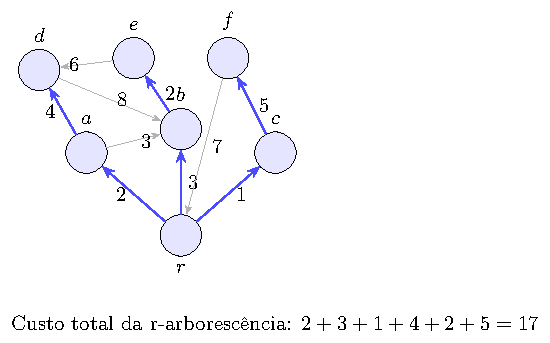
\includegraphics[width=0.9\linewidth]{figures/fig_r_arborescencia_custo_minimo.pdf}

    \caption{r-arborescência de custo mínimo: arborescência enraizada em $r$ que minimiza a soma dos custos dos arcos, em azul. No exemplo, o custo total é $17$. Em cinza, arcos que não fazem parte da r-arborescência de custo mínimo.}
    \label{fig:r-arborescencia-custo-minimo}\end{figure}


\paragraph{r-arborescência inversa de custo mínimo:}
é uma arborescência inversa enraizada em um vértice específico \(r\) que minimiza a soma dos pesos dos arcos que a compõem. Formalmente, dada uma função de custo \(c: A \to \mathbb{R}_{\geq 0}\) que atribui um custo a cada arco do dígrafo \(D = (V, A)\), uma r-arborescência inversa de custo mínimo \(T\) é uma arborescência inversa \(T = (V_T, A_T)\) onde \(V_T \subseteq V\) e \(A_T \subseteq A\), que satisfaz as seguintes propriedades:
\begin{itemize}
    \item \(T\) é uma arborescência inversa enraizada em \(r\): existe um caminho direcionado de qualquer vértice em \(V_T\) até \(r\).
    \item \(T\) minimiza o custo total: a soma dos custos dos arcos em \(A_T\) é mínima, ou seja, \(\sum_{a \in A_T} c(a)\) é minimizada.
\end{itemize}

\paragraph{}

\begin{figure}[H]
    \centering
    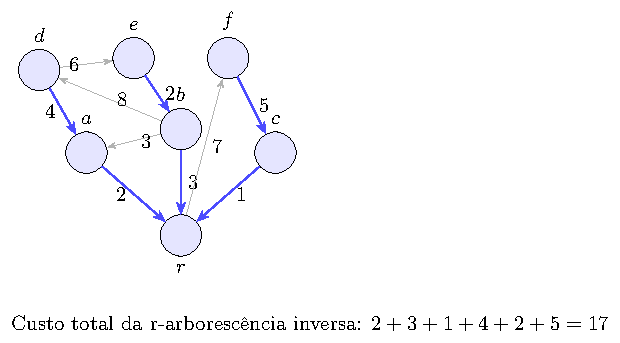
\includegraphics[width=0.9\linewidth]{figures/fig_r_arborescencia_inversa_custo_minimo.pdf}

    \caption{r-arborescência inversa de custo mínimo: arborescência inversa enraizada em $r$ que minimiza a soma dos custos dos arcos, em azul. No exemplo, o custo total é $17$. Em cinza, arcos que não fazem parte da r-arborescência inversa de custo mínimo.}
    \label{fig:r-arborescencia-inversa-custo-minimo}\end{figure}


\paragraph{}
As arborescências são a principal estrutura que exploraremos ao longo desta dissertação, especialmente a r-arborescência de custo mínimo e r-arborescência inversa de custo mínimo, abordaremos o problema de encontrá-las eficientemente em dígrafos com custos associados aos arcos.



\paragraph{Noções aprofundadas em arborescências}

\paragraph{}
Vamos explorar algumas propriedades e teoremas importantes relacionados a arborescências, que serão úteis para entender os algoritmos que discutiremos posteriormente.

\paragraph{Grau e contagem de arcos:}
\paragraph{}
Seja $T$ uma out-arborescência enraizada em $r$ com $n$ vértices. Ela é exatamente a estrutura que satisfaz as três condições combinadas abaixo (todas muito fáceis de checar):
\begin{enumerate}\setlength{\itemsep}{2pt}
    \item (Contagem) $|A_T| = n-1$.
    \item (Entrada única) Cada vértice $v\neq r$ recebe exatamente um arco: $d_T^-(v)=1$.
    \item (Raiz sem entrada) A raiz não recebe arcos: $d_T^-(r)=0$.
\end{enumerate}
De forma simétrica, numa in-arborescência (arborescência inversa) valem as versões “espelhadas”: cada $v\neq r$ tem exatamente um arco \emph{saindo} ($d_T^+(v)=1$) e a raiz tem grau de saída zero ($d_T^+(r)=0$).

\paragraph{}
Reciprocamente, qualquer subdígrafo que satisfaça (1)--(3) é uma out-arborescência enraizada em $r$ (e análogamente no caso inverso). 

\paragraph{Discussões importantes sobre arborescências}

\paragraph{}
Dado um Dígrafo \(D = (V, A)\) e um vértice raiz \(r \in V\), uma questão fundamental é determinar quando existe uma arborescência enraizada em \(r\).
Existem alguns resultados clássicos que caracterizam a existência de arborescências em dígrafos, bem como condições para a existência de múltiplas arborescências disjuntas. Vamos apresentar dois teoremas fundamentais nesse contexto.

\paragraph{Teorema de Fulkerson}

\paragraph{}
Existem várias formas de caracterizar a existência de arborescências em um dígrafo. Uma delas é via a condição de cortes, que estabelece uma relação entre a existência de arborescências e a estrutura dos cortes no dígrafo.

\paragraph{}
Esse resultado é conhecido como o \textbf{Teorema de Fulkerson} e para entendermos ele precisamos ter em mente as seguintes definições:

\begin{itemize}
    \item Seja \(D = (V, A)\) um dígrafo e \(X \subseteq V\) um subconjunto de vértices. O conjunto \(\delta^-(X)\) é definido como o conjunto de todos os arcos que entram em \(X\) vindos de \(V \setminus X\). Formalmente,
    \[
    \delta^-(X) = \{(u, v) \in A : u \in V \setminus X, v \in X\}.
    \]
    \item Um corte em um dígrafo é uma partição dos vértices em dois subconjuntos disjuntos. O conjunto \(\delta^-(X)\) representa o corte que separa \(X\) do resto do grafo.
\end{itemize}

\paragraph{}
A seguir apresentamos o teorema propriamente dito e um esboço de sua prova.

\paragraph{}
\begin{teobox}{Condição de existência via cortes (Fulkerson)}{fulkerson-existencia}
Seja $D=(V,A)$ e $r\in V$. Existe uma out-arborescência (arborescência dirigida) enraizada em $r$ se, e somente se,
\[
\forall\, X\subseteq V\setminus\{r\},\ X\neq\emptyset:\  \delta^-(X)\neq\emptyset.
\]
Isto é: todo subconjunto não vazio que não contém a raiz recebe ao menos um arco vindo de fora.

\paragraph{}
	\textbf{Prova (esboço):} 

\paragraph{}
\emph{(Só se:)} Suponha que $T$ é uma out-arborescência enraizada em $r$. Pegue qualquer $X\neq\emptyset$ sem $r$. Considere o primeiro vértice de $X$ alcançado a partir de $r$ no caminho dentro de $T$; o arco imediatamente anterior entra em $X$ e pertence a $\delta^-(X)$. Logo $\delta^-(X)\neq\emptyset$.

\paragraph{}
\emph{(Se:)} Agora suponha que toda parte $X$ não vazia sem $r$ recebe um arco. Construímos $T$ iterativamente: comece com $S=\{r\}$. Enquanto $S\neq V$, tome um vértice $v\in V\setminus S$ tal que existe um arco $(u,v)$ com $u\in S$ (existe porque, caso contrário, o conjunto $X=V\setminus S$ não receberia arco). Adicione $v$ e o arco $(u,v)$. Não criamos ciclos porque cada novo vértice entra com exatamente um arco e só aponta para frente (a direção é de um vértice já inserido para um novo). Ao final, cada $v\neq r$ tem exatamente um arco de entrada e o grafo é conexo a partir de $r$, logo obtivemos uma out-arborescência.

\medskip
	\textbf{Intuição curta.} A condição “todo $X$ tem um arco entrando” impede que qualquer bloco de vértices fique isolado da raiz; o processo guloso de anexar o primeiro arco que entra em cada bloco produz a arborescência sem retrocessos.

\medskip
\emph{Referência:} ver, por exemplo, \cite{schrijver2003comb}.
\label{thm:fulkerson-cut-arborescencia}
\end{teobox}

\paragraph{}
Outro resultado clássico é o teorema que caracteriza a existência de múltiplas arborescências arcodisjuntas em um dígrafo, conhecido como o \textbf{Teorema de Edmonds}. Precisamos de algumas definições antes de enunciá-lo:

\begin{itemize}
    \item Duas arborescências são ditas \emph{arcodisjuntas} se não compartilham nenhum arco, ou seja, \(A_{T_1} \cap A_{T_2} = \emptyset\).
    \item A condição de cortes para múltiplas arborescências estabelece que, para qualquer subconjunto \(X \subseteq V \setminus \{r\}\), o número de arcos que entram em \(X\) deve ser pelo menos igual ao número de arborescências desejadas.
    \item Uma out-arborescência enraizada em \(r\) é uma arborescência onde todos os caminhos direcionados partem de \(r\) e alcançam todos os outros vértices.
    \item O conjunto \(\delta^-(X)\) é definido como o conjunto de todos os arcos que entram em \(X\) vindos de \(V \setminus X\). Formalmente,
    \[
    \delta^-(X) = \{(u, v) \in A : u \in V \setminus X, v \in X\}.
    \]
    \item Um corte em um dígrafo é uma partição dos vértices em dois subconjuntos disjuntos. O conjunto \(\delta^-(X)\) representa o corte que separa \(X\) do resto do grafo.
    \end{itemize}

\paragraph{}
Antes de enunciar o teorema, vale a pena mencionar o conceito de \emph{interseção de matroides}, mas, para não alongar demais, deixamos a explicação detalhada para o Apêndice \ref{ap:matroides}. Aqui, apenas uma breve introdução:
\begin{itemize}
    \item Matroides, são estruturas combinatórias que generalizam a noção de independência linear em álgebra linear. A interseção de matroides é um conceito que permite combinar duas ou mais estruturas de matroides para formar uma nova estrutura que mantém certas propriedades de independência.
    \item A interseção de matroides é frequentemente utilizada em problemas de otimização combinatória, onde é necessário encontrar soluções que satisfaçam múltiplas condições de independência simultaneamente.
    \item Familia de conjuntos independentes: cada matroide é definido por uma coleção de subconjuntos de um conjunto finito, chamados de conjuntos independentes, que satisfazem certas propriedades.
    \item No contexto de arborescências, a interseção de matroides pode ser usada para modelar a seleção de arcos que formam múltiplas arborescências arcodisjuntas, garantindo que cada arborescência mantenha suas propriedades de independência.
\end{itemize}

\paragraph{}

\begin{figure}[H]
    \centering
    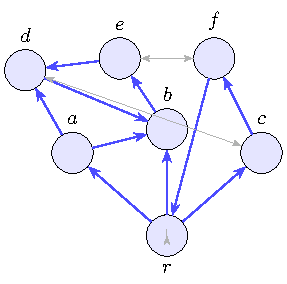
\includegraphics[width=0.9\linewidth]{figures/fig_exemplo_multiplas_arborescencias.pdf}

    \caption{Dígrafo de exemplo para múltiplas arborescências arcodisjuntas.}
    \label{fig:exemplo-multiplas-arborescencias}\end{figure}


\paragraph{}
Agora podemos enunciar o teorema de Edmonds, que fornece uma condição necessária e suficiente para a existência de \(k\) arborescências arcodisjuntas enraizadas em um vértice \(r\).

\paragraph{}
\begin{teobox}{$k$ arborescências arcodisjuntas (Edmonds)}{edmonds-k-arborescencias}
Seja $D=(V,A)$, $r\in V$ e $k\ge 1$ inteiro. São equivalentes:
\begin{enumerate}\setlength{\itemsep}{4pt}
    \item Existem $k$ out-arborescências enraizadas em $r$ que são par a par \emph{arcodisjuntas}.
    \item (Condição de cortes) Para todo subconjunto $X\subseteq V\setminus\{r\}$ vale $|\delta^-(X)| \ge k$.
\end{enumerate}
Em palavras: cada “bloco” $X$ que não contém a raiz precisa ter pelo menos $k$ arcos distintos chegando de fora; isso é exatamente o que permite "alimentar" $X$ a partir de $r$ em $k$ estruturas de ramificação independentes.

\paragraph{}
\textbf{Prova (esboço):}
\emph{(1 $\Rightarrow$ 2)} Se temos $k$ out-arborescências arcodisjuntas, então cada arborescência deve entrar em qualquer $X$ (senão não alcançaria seus vértices). Como os arcos são distintos entre as $k$ estruturas, precisamos de pelo menos $k$ arcos entrando em $X$; logo $|\delta^-(X)|\ge k$.

\paragraph{}
\emph{(2 $\Rightarrow$ 1)} Trata-se a construção como um problema de \emph{interseção de matroides} ou aplicamos um procedimento incremental de troca ("augmenting"). O conjunto de arcos pode suportar no máximo $k(n-1)$ arcos selecionados se quisermos $k$ arborescências, onde cada vértice $v \neq r$ recebe exatamente $k$ arcos de entrada (um de cada arborescência). A condição de cortes impede gargalos: se algum subconjunto $X$ tivesse menos que $k$ arcos entrando, seria impossível abastecer seus vértices com $k$ escolhas independentes.

\paragraph{}
Uma prova clássica (Edmonds) formula o problema como interseção de duas famílias independentes: 

\paragraph{}
(i) uma família que limita a quantidade de arcos entrando em cada vértice a no máximo $k$; 

\paragraph{}
(ii) uma família que evita a criação de ciclos dirigidos ao selecionar arcos (estrutura de matroide de partição + matroide gráfico orientado). 

\paragraph{}
A hipótese de cortes garante que o algoritmo de aumento (que tenta adicionar um arco e, se criar ciclo ou saturar um vértice, realiza trocas) nunca fica travado antes de atingir $k(n-1)$ arcos. Agrupando, particionamos esses $k(n-1)$ arcos em $k$ coleções de $(n-1)$ arcos cada, que formam as $k$ out-arborescências arcodisjuntas.

\medskip
\emph{Referências:} Edmonds (teorema das branchings) \cite{edmonds1967optimum}, apresentações modernas em \cite{schrijver2003comb}.
\label{thm:edmonds-disjoint-arborescencias} 
\end{teobox}

\paragraph{}
Teoremas como esses servem para responder perguntas do tipo “quando existe?” e “quão rica pode ser a estrutura?”. Em particular, eles nos dizem que:
\begin{itemize}\setlength{\itemsep}{2pt}
    \item A existência de uma arborescência enraizada em \(r\) é garantida se, e somente se, todo subconjunto não vazio que não contém \(r\) recebe pelo menos um arco vindo de fora (Teorema de Fulkerson).
    \item A existência de \(k\) arborescências arcodisjuntas enraizadas em \(r\) é garantida se, e somente se, todo subconjunto não vazio que não contém \(r\) recebe pelo menos \(k\) arcos vindos de fora (Teorema de Edmonds).
\end{itemize}

\paragraph{}
Mas, agora estamos interessados em achar essas arborescências de forma eficiente, especialmente quando os arcos têm custos associados. Queremos encontrar a r-arborescência de custo mínimo, ou seja, a arborescência enraizada em \(r\) que minimiza a soma dos custos dos arcos que a compõem.

\paragraph{}
Um resultado central agora é a caracterização de \emph{optimalidade} para r-arborescências de custo mínimo: as chamadas \emph{condições de Fulkerson}. Elas conectam a solução primal (os arcos escolhidos) a um certificado dual (potenciais em subconjuntos) via custos reduzidos.

\paragraph{Terminologia:} 
\paragraph{}
Para um dígrafo $D=(V,A)$, raiz $r$ e custos $c:A\to \mathbb{R}_{\ge 0}$, um subconjunto não vazio $X\subseteq V\setminus\{r\}$ é dito \textbf{apertado} (para uma família de pesos $y$) se exatamente um arco da solução escolhida entra em $X$ e $y(X)>0$. 

\paragraph{}
Diremos que um arco $a=(u,v)$ \emph{entra} em $X$ se $u\notin X$ e $v\in X$. 

\paragraph{}
Dada uma família de pesos $y: \{X\subseteq V\setminus\{r\}: X\neq\emptyset\}\to \mathbb{R}_{\ge 0}$, definimos o \textbf{custo reduzido} de $a$ por
\[
 c'(a) \;=\; c(a)\; - \sum_{\substack{X\subseteq V\setminus\{r\},\\ X\neq\emptyset,\ u\notin X,\ v\in X}} y(X).
\]

\paragraph{}
\begin{teobox}{Optimalidade de Fulkerson (r-arborescência de custo mínimo)}{fulkerson-opt}
Seja $D=(V,A)$, raiz $r$ e custos $c:A\to\mathbb{R}_{\ge 0}$. Seja $T$ uma out-arborescência enraizada em $r$. As afirmações são equivalentes: 
\begin{enumerate}\setlength{\itemsep}{4pt}
    \item $T$ tem custo mínimo entre todas as out-arborescências enraizadas em $r$.
    \item Existem pesos $y(X)\ge 0$ para cada $\emptyset\neq X\subseteq V\setminus\{r\}$ tais que:
    \begin{enumerate}\setlength{\itemsep}{2pt}
         \item[(a)] $c'(a)\ge 0$ para todo arco $a\in A$ (não negatividade dos custos reduzidos);
         \item[(b)] $c'(a)=0$ para todo arco $a\in T$ (complementaridade em arcos usados);
         \item[(c)] Para todo $X$ com $y(X)>0$ entra \emph{exatamente um} arco de $T$ em $X$ (complementaridade em conjuntos apertados).
    \end{enumerate}
\end{enumerate}
Além disso, quando (2) vale, o valor $\sum_X y(X)$ é exatamente o custo de $T$.

\paragraph{}
	\textbf{Prova (esboço):}

\paragraph{(2 $\Rightarrow$ 1).} Para qualquer arborescência $B$ temos
\[
 	\textbf{custo}(B) = \sum_{a\in B} c(a) = \sum_{a\in B} \Big( c'(a) + \sum_{X: a\text{ entra }X} y(X) \Big).
\]
Trocando a ordem da soma:
\[
 	\textbf{custo}(B) = \sum_{a\in B} c'(a) + \sum_X y(X)\,\big| \{a\in B: a \text{ entra } X\}\big|.
\]
Pelas condições, $c'(a)\ge 0$, logo a primeira soma é $\ge 0$. Como uma out-arborescência entra em qualquer $X\neq\emptyset$ (senão $X$ estaria desconectado de $r$), temos $|\{a\in B: a \text{ entra } X\}|\ge 1$. Assim
\[
 	\textbf{custo}(B) \ge \sum_X y(X).
\]
Para $B=T$, pela complementaridade $c'(a)=0$ se $a\in T$ e para cada $X$ com $y(X)>0$ entra \emph{exatamente} um arco de $T$, obtendo
\[
 	\textbf{custo}(T) = 0 + \sum_X y(X),
\]
logo $\textbf{custo}(T) \le \textbf{custo}(B)$ para qualquer $B$; $T$ é ótimo.

\paragraph{(1 $\Rightarrow$ 2).} (Ideia) Execute o procedimento clássico: enquanto houver vértice (ou componente contraída) $v\neq r$ sem arco de custo reduzido zero entrando, subtraia do custo de todos os arcos que entram em $v$ o menor custo positivo entre eles (isso equivale a aumentar uniformemente $y(X)$ para cada subconjunto $X$ cujo primeiro arco zero estamos “criando”). Quando um ciclo de arcos de custo reduzido zero surge, contraia-o e continue no dígrafo comprimido. Ao final, os arcos de custo reduzido zero selecionados formam $T$. As quantidades subtraídas definem $y$: cada vez que subtraímos $\alpha>0$ para um subconjunto/componente $X$, somamos $\alpha$ a $y(X)$. Construção garante (a)–(c).

\paragraph{Intuição.} Os pesos $y$ “pagam” parcialmente cada arco de fora para dentro dos subconjuntos; arcos da solução ficam exatamente “quitados” (custo reduzido 0). Se algum arco restante tivesse custo reduzido negativo, poderíamos baixar o custo da solução trocando-o por um arco de $T$, contradizendo optimalidade. Conjuntos com $y(X)>0$ exigem uso único de um arco para não desperdiçar potencial.

\medskip
\emph{Referências:} Fulkerson (condições de optimalidade), apresentações modernas em \cite{frank2014, schrijver2003comb}.
\label{thm:fulkerson-optimalidade-arborescencia}
\end{teobox}

\paragraph{}
O teorema anterior nos diz como reconhecer, de forma concreta, que a arborescência encontrada é realmente de custo mínimo. Fazemos uma normalização simples de custos\footnote{Por “normalização de custos” entendemos subtrair a mesma constante de todos os arcos que entram em um mesmo subconjunto (ou componente) do grafo, para simplificar os valores e criar arcos de custo reduzido zero, sem alterar qual solução é ótima; em outras palavras, trabalhar com custos reduzidos.}: para cada “parte” do grafo, subtraímos, dos arcos que entram nessa parte, o menor custo observado; com isso, pelo menos um arco que entra em cada parte zera. A solução ótima pode ser construída usando apenas arcos com custo reduzido zero e, sob esse ajuste, não sobra nenhuma troca que diminua o custo.

\paragraph{}
Na prática, a verificação de optimalidade se reduz a checar condições locais:
\begin{itemize}\setlength{\itemsep}{2pt}
    \item não há arcos com custo reduzido negativo;
    \item todo arco que compõe a arborescência tem custo reduzido zero;
    \item para cada conjunto “apertado” (isto é, que recebeu desconto positivo no ajuste), entra exatamente um arco da arborescência.
\end{itemize}
Se alguma dessas condições falhar, existe uma troca que barateia a solução; se todas forem satisfeitas, temos um certificado de optimalidade curto e fácil de verificar.

\paragraph{}
Com essa ideia em mãos, saímos do “o que é ótimo?” para “como chegar lá, passo a passo?”. No próximo capítulo apresentamos a noção de algoritmo que adotaremos e descrevemos os métodos clássicos para este problema: o algoritmo de Chu–Liu/Edmonds (que cria arcos de custo zero e contrai ciclos) e o procedimento em duas fases de András Frank. Veremos as etapas, a intuição por trás e como vamos implementá-los no projeto.

\subsection{Algoritmos}
\paragraph{}
Quando falamos em passo a passo é muito comum vir à mente a ideia de receitas de cozinha, instruções de montagem ou manuais de operação. Em ciência da computação, o termo \emph{algoritmo} captura essa ideia de forma mais formal e precisa.

\paragraph{}O primeiro uso documentado do termo “algoritmo” em inglês data de 1230, em uma tradução latina do trabalho de Al-Khwarizmi. No entanto, o conceito de algoritmos é muito mais antigo, remontando a procedimentos matemáticos e lógicos desenvolvidos ao longo dos séculos.

\paragraph{}
Um dos primeiros algoritmos conhecidos é o \emph{método de Euclides} para encontrar o máximo divisor comum (mdc) de dois números inteiros, descrito por Euclides em sua obra "Os Elementos" por volta de 300 a.C. 

\paragraph{}
\begin{algobox}{Método de Euclides (mdc)}{mdc}
Dados inteiros positivos $a$ e $b$:
\begin{enumerate}\setlength{\itemsep}{2pt}
    \item enquanto $b>0$, substitua $(a,b)$ por $(b, a\bmod b)$;
    \item quando $b=0$, devolva $a$.
\end{enumerate}
\end{algobox}

\paragraph{}
Mas, o que diferencia uma mera receita de um algoritmo? A resposta está na clareza, precisão e capacidade de execução repetitiva das instruções. Um algoritmo deve ser:
\begin{itemize}\setlength{\itemsep}{2pt}
    \item \textbf{Não ambiguidade}: cada passo deve ser definido de maneira inequívoca, sem ambiguidade.
    \item \textbf{Especificidade}: as instruções devem ser detalhadas o suficiente para que possam ser seguidas sem interpretação subjetiva.
    \item \textbf{Executabilidade}: deve ser possível executar o algoritmo de forma sistemática, sem necessidade de criatividade ou intuição.
\end{itemize}

\paragraph{}
Por isso, que chamamos o método de Euclides de algoritmo: os passos são não ambíguos; termina porque a segunda coordenada diminui até zerar; é correto pois mantém o invariante $\gcd(a,b)=\gcd(b,a\bmod b)$; e o custo é baixo (proporcional ao número de dígitos de $a$ e $b$).

\paragraph{}
Além dessas características, precisamos citar mais alguns conceitos úteis na análise de algoritmos:
\begin{itemize}\setlength{\itemsep}{2pt}
    \item \textbf{Invariante}: uma propriedade que permanece verdadeira durante a execução do algoritmo. Por exemplo, em um algoritmo de ordenação, um invariante pode ser que os elementos à esquerda de um índice específico estão sempre ordenados. (ex.: “não há custos reduzidos negativos” ou “cada componente tem ao menos um arco zero entrando”).
    \item \textbf{Correção}: a garantia de que o algoritmo produz a saída correta para todas as entradas válidas. Isso geralmente é demonstrado por meio de provas formais ou argumentos lógicos. (ex.: justificativa de que o resultado final é uma arborescência válida e de custo mínimo)
    \item \textbf{Terminação}: a garantia de que o algoritmo sempre chegará a um ponto final, ou seja, que não entrará em um loop infinito. Isso pode ser demonstrado mostrando que alguma medida (como o tamanho da entrada) diminui a cada passo. (ex.: cada contração reduz $|V|$; cada ajuste cria um novo arco zero).
\end{itemize}

\paragraph{}
Essas características não definem formalmente o que é um algoritmo, mas ajudam a entender o conceito. A definição formal envolve a ideia de \emph{computabilidade}\footnote{A computabilidade é um conceito na teoria da computação, que se refere à capacidade de um problema ser resolvido por um algoritmo em um tempo finito. \emph{Comentário formal.} Esse conceito é formalizado por meio de modelos como máquinas de Turing, funções recursivas, RAM, entre outros. Essas formalizações são equivalentes quanto ao que é computável (Tese de Church–Turing) e permitem discutir com rigor correção e complexidade (tempo e memória).}, e isso envolve uma discussão profunda demais para o escopo deste trabalho.

\subsubsection{Complexidade de Algoritmos}

\paragraph{}
Porém, precisamos nos aprofunda em um dos conceitos que estão envolvidos em computabilidade: o de \emph{complexidade de algoritmos}, que se refere à quantidade de recursos computacionais (tempo e espaço) que um algoritmo consome em função do tamanho da entrada.

\paragraph{}
A complexidade de um algoritmo pode ser analisada em termos de \emph{complexidade de tempo} e \emph{complexidade de espaço}. A complexidade de tempo refere-se ao tempo que um algoritmo leva para ser executado, enquanto a complexidade de espaço refere-se à quantidade de memória que um algoritmo utiliza durante sua execução.

\paragraph{}
A notação assintótica é frequentemente usada para expressar a complexidade de algoritmos, permitindo descrever o comportamento do algoritmo à medida que o tamanho da entrada cresce. As notações mais comuns são:
\begin{itemize}\setlength{\itemsep}{2pt}
    \item \textbf{O grande (Big O)}: descreve um limite superior para o crescimento da função. Por exemplo, se um algoritmo tem complexidade \(O(n^2)\), isso significa que o tempo de execução do algoritmo cresce no máximo proporcional a \(n^2\) para entradas grandes.
    \item \textbf{Ômega (\(\Omega\))}: descreve um limite inferior para o crescimento da função. Se um algoritmo tem complexidade \(\Omega(n)\), isso significa que o tempo de execução do algoritmo cresce no mínimo proporcional a \(n\) para entradas grandes.
    \item \textbf{Theta (\(\Theta\))}: descreve um limite assintótico preciso, indicando que a função cresce exatamente proporcional a uma determinada função. Se um algoritmo tem complexidade \(\Theta(n \log n)\), isso significa que o tempo de execução do algoritmo cresce proporcional a \(n \log n\) para entradas grandes.
\end{itemize}

\paragraph{}
Essas notações ajudam a comparar a eficiência de diferentes algoritmos e a entender como eles se comportam à medida que o tamanho da entrada aumenta\footnote{Por “tamanho da entrada” entendemos a quantidade de símbolos necessária para codificar a instância (tipicamente, o número de bits). Exemplos: (i) para grafos, mede-se usualmente por \(n=|V|\) e \(m=|E|\); se há pesos, também se contabiliza o número de bits para representá-los; (ii) para inteiros, é o número de dígitos; (iii) para strings, o comprimento. Em análises de alto nível, é comum expressar custos como funções de \(n\) e \(m\) no modelo RAM (palavra de \(\Theta(\log n)\) bits), mas quando os pesos são grandes a complexidade em bits pode prevalecer.}. Ao analisar a complexidade de um algoritmo, é importante considerar o pior caso, o caso médio e o melhor caso, dependendo do contexto em que o algoritmo será utilizado.

\paragraph{}
Para ilustrar a análise de complexidade, consideremos o exemplo da busca linear vs busca binária em um vetor ordenado\footnote{Por vetor ordenado entendemos um arranjo (array) em que os elementos estão armazenados em posições consecutivas e dispostos segundo uma ordem total (tipicamente crescente ou não decrescente). Essa organização permite algoritmos como a busca binária, que dependem de comparações para descartar metades do intervalo.}. 

\paragraph{Exemplo: Busca Linear vs Busca Binária}
\paragraph{}
O algoritmo de busca linear percorre cada elemento do vetor até encontrar o valor desejado ou chegar ao final do vetor. A complexidade desse algoritmo é \(O(n)\) no pior caso, onde \(n\) é o tamanho do vetor, pois pode ser necessário verificar todos os elementos.

\begin{algobox}{Busca Linear}{busca-linear}
Dado um vetor \(V\) de tamanho \(n\) e um valor \(x\):
\begin{enumerate}\setlength{\itemsep}{2pt}
    \item Para cada índice \(i\) de \(0\) a \(n - 1\):
    \begin{enumerate}\setlength{\itemsep}{2pt}
        \item Se \(V[i] = x\), retorne \(i\).
    \end{enumerate}
    \item Retorne \(-1\) (indica que \(x\) não está no vetor).
\end{enumerate}
\end{algobox}

\paragraph{}
Já o algoritmo de busca binária aproveita o fato de que o vetor está ordenado para reduzir o espaço de busca pela metade a cada iteração.

\begin{algobox}{Busca Binária}{busca-binaria}
Dado um vetor ordenado \(V\) de tamanho \(n\) e um valor \(x\):
\begin{enumerate}\setlength{\itemsep}{2pt}
    \item Defina \(\text{início} = 0\) e \(\text{fim} = n - 1\).
    \item Enquanto \(\text{início} \leq \text{fim}\):
    \begin{enumerate}\setlength{\itemsep}{2pt}
        \item Calcule \(meio = \left\lfloor \dfrac{\text{início} + \text{fim}}{2} \right\rfloor\).
        \item Se \(V[meio] = x\), retorne \(meio\).
        \item Se \(V[meio] < x\), defina \(\text{início} = meio + 1\).
        \item Caso contrário, defina \(\text{fim} = meio - 1\).
    \end{enumerate}
    \item Retorne \(-1\) (indica que \(x\) não está no vetor).
\end{enumerate}
\end{algobox}  

O algoritmo de busca linear tem a seguinte complexidade:
\begin{itemize}\setlength{\itemsep}{2pt}
    \item \textbf{Melhor caso}: \(O(1)\) - o elemento procurado está na primeira posição.
    \item \textbf{Caso médio}: \(O(n)\) - em média, metade dos elementos precisam ser verificados.
    \item \textbf{Pior caso}: \(O(n)\) - o elemento procurado está na última posição ou não está no vetor.
\end{itemize}

Já o algoritmo de busca binária tem a seguinte complexidade:
\begin{itemize}\setlength{\itemsep}{2pt}
    \item \textbf{Melhor caso}: \(O(1)\) - o elemento procurado está no meio do vetor.
    \item \textbf{Caso médio}: \(O(\log n)\) - em média, a cada iteração, o tamanho do vetor é reduzido pela metade.
    \item \textbf{Pior caso}: \(O(\log n)\) - o elemento procurado não está no vetor ou está na extremidade.
\end{itemize}
 
\paragraph{}
Esse exemplo ilustra como a análise de complexidade pode fornecer insights sobre a eficiência de um algoritmo em diferentes cenários. A busca binária é muito mais eficiente do que uma busca linear (\(O(n)\)) para grandes vetores, graças à sua capacidade de reduzir o espaço de busca pela metade a cada iteração.

\subsubsection{Os problemas e suas complexidades}

Não avaliamos só o desempenho de \emph{um algoritmo}; também queremos saber \emph{quão difícil é o próprio problema}, assim temos  a seguinte forma de classificar problemas:    
\begin{itemize}\setlength{\itemsep}{2pt}
    \item \textbf{Problemas de decisão}: problemas que podem ser respondidos com "sim" ou "não". Ex.: "Existe um caminho entre dois vértices em um grafo?"
    \item \textbf{Problemas de otimização}: problemas que envolvem encontrar a melhor solução possível entre várias opções. Ex.: "Qual é o caminho mais curto entre dois vértices em um grafo ponderado?"
    \item \textbf{Problemas de contagem}: problemas que envolvem contar o número de soluções possíveis. Ex.: "Quantos caminhos existem entre dois vértices em um grafo?"
\end{itemize}

\paragraph{}
Cada classe de problemas pode ter diferentes níveis de dificuldade, que avaliamos em termos de \emph{complexidade computacional}, que mede os recursos necessários (tempo e espaço) para resolver o problema.

Problemas são considerados "fáceis" quando são resolvíveis em tempo polinomial, enquanto outros são "difíceis" quando não se conhece nenhum algoritmo eficiente para resolvê-los.

\paragraph{Classes de complexidade de problemas}

\paragraph{}
 Como regra prática, consideramos \emph{tratáveis} os problemas que admitem soluções em tempo (ou espaço) \emph{polinomial} no tamanho da entrada e \emph{intratáveis} os que não admitem. Essa distinção é formalizada por meio de \emph{classes de complexidade}, que agrupam problemas segundo sua dificuldade intrínseca. Abaixo apresentamos-as:

\begin{itemize}\setlength{\itemsep}{2pt}
    \item \textbf{P} (tempo polinomial). “Resolver é fácil”: existe um algoritmo que encontra a resposta em tempo que cresce como \(n^k\) para algum \(k\). Exemplos: conectividade em grafos, árvore geradora mínima (MST), caminho mínimo com pesos não negativos, fluxo máximo.
    \item \textbf{NP} (verificação polinomial). “Conferir é fácil”: se alguém propõe uma solução, conseguimos \emph{verificar} em tempo polinomial se ela está correta (achar pode ser difícil). Exemplos: \emph{SAT} (satisfatibilidade booleana), \emph{Clique}, \emph{Vertex Cover}.
    \item \textbf{co-NP}. Complementos dos problemas em NP — “conferir o ‘não’ é fácil” em vez do “sim”. Exemplo: \emph{TAUT} (verificar se uma fórmula é tautologia) está em co-NP.
    \item \textbf{NP-difícil}. “Tão difíceis quanto o mais difícil de NP”: todo problema de NP reduz-se (em tempo polinomial) a eles. Podem ser de decisão, otimização ou contagem e \emph{não precisam} estar em NP. Em geral, não se espera algoritmo polinomial para todos os casos. Exemplos: versão de otimização do \emph{TSP} (caixeiro-viajante), programação inteira, coloração mínima de grafos.
    \item \textbf{NP-completo}. “Os mais difíceis \emph{dentro} de NP”: problemas de decisão que estão em NP e são NP-difíceis. Se algum NP-completo tiver algoritmo polinomial, então \(\mathrm{P}=\mathrm{NP}\). Exemplos: \emph{SAT}, \emph{3-SAT}, problema \emph{Hamiltoniano} (existe ciclo hamiltoniano?).
    \item \textbf{PSPACE} (espaço polinomial). “Memória polinomial, tempo possivelmente enorme”: resolvíveis usando memória que cresce polinomialmente com o tamanho da entrada. Exemplo: \emph{QBF} (satisfatibilidade com quantificadores) é PSPACE-completo.
\end{itemize}

\paragraph{Reduções polinomiais}

\paragraph{}
Para comparar dificuldades, usamos reduções de problemas, reduzimos o problema \(A\) ao problema \(B\) (escrevemos \(A\le_p B\)) quando conseguimos transformar qualquer instância de \(A\) em uma instância de \(B\) em tempo polinomial, de modo que resolver \(B\) nos dê a resposta de \(A\) com apenas um sobrecusto polinomial. Logo: se \(A\le_p B\), então \textbf{\(B\) é pelo menos tão difícil quanto \(A\)} (um resolvedor para \(B\) resolveria \(A\) via redução). \footnote{Consequência útil: se \(A\le_p B\) e \(B\) tem algoritmo polinomial, então \(A\) também tem. Para mostrar que um problema \(C\) é NP-difícil, reduzimos \emph{de} um NP-completo conhecido \(P\) \emph{para} \(C\) (isto é, \(P\le_p C\)). Para provar que \(C\) é NP-completo, além disso precisamos que \(C\in\mathrm{NP}\). Exemplo: \(\text{3-SAT}\le_p \text{Clique}\) — resolver \textit{Clique} eficientemente daria um método eficiente para \textit{3-SAT}.}

\paragraph{Relações conhecidas}

\paragraph{}
Temos inclusões básicas: \(\mathrm{P}\subseteq \mathrm{NP}\), \(\mathrm{P}\subseteq \mathrm{co\text{-}NP}\) e \(\mathrm{NP}\subseteq \mathrm{PSPACE}\subseteq \mathrm{EXP}\). Acredita-se que muitas dessas inclusões sejam estritas, mas isso não foi provado; em particular, o problema \(\mathrm{P}\) vs \(\mathrm{NP}\) permanece em aberto. Também não se sabe se \(\mathrm{NP}=\mathrm{co\text{-}NP}\).

\paragraph{}
Essas classes não só categorizam problemas por sua dificuldade intrínseca, como também orientam a \emph{estratégia de solução}. Em linhas gerais: (i) quando o problema está em \(\mathrm{P}\), preferimos \textbf{algoritmos exatos} com tempo polinomial; (ii) para problemas NP-completos/NP-difíceis, \emph{não se conhecem} algoritmos exatos polinomiais (a menos que \(\mathrm{P}=\mathrm{NP}\)), e métodos gerais costumam ter pior caso exponencial. Por isso, são comuns \textbf{heurísticas}, \textbf{algoritmos de aproximação} e abordagens de \textbf{complexidade parametrizada} (FPT), além de algoritmos \textbf{pseudo-polinomiais} em casos numéricos. Muitas vezes, estruturas especiais (ex.: largura de árvore pequena, aciclicidade, graus limitados) também permitem soluções exatas polinomiais para subclasses. A seguir, explicitamos essa distinção entre \emph{algoritmos exatos} e \emph{heurísticas}.

\subsubsection{Tipificando Algoritmos}

É comum ouvirmos que “o ótimo é inimigo do bom”. Essa frase, atribuída a Voltaire, expressa a ideia de que buscar a perfeição pode impedir que se alcance um resultado satisfatório. Essa tensão entre buscar o ideal do “ótimo”  ou aceitar o “suficientemente bom” quando recursos e tempo são limitados\footnote{Na teoria da decisão, essa postura pragmática é conhecida como \emph{satisficing}, termo introduzido por Herbert A. Simon.} essa noção se materializa em uma forma de tipificação de algoritmos.

\paragraph{Algoritmos Exatos vs Heurísticos}

\paragraph{}
Essa distinção é especialmente relevante em problemas de otimização, onde o objetivo é encontrar a melhor solução possível entre um conjunto de soluções viáveis. Existem dois tipos principais de algoritmos para abordar esses problemas: os \emph{algoritmos exatos} e os \emph{algoritmos heurísticos}.

\begin{itemize}\setlength{\itemsep}{2pt}
    \item \textbf{Algoritmos Exatos}: são aqueles que garantem encontrar a solução ótima para um problema, se uma solução existe. Eles exploram todas as possibilidades ou utilizam técnicas matemáticas rigorosas para garantir a optimalidade. Exemplos incluem algoritmos de programação linear, algoritmos de busca exaustiva e algoritmos baseados em teoria dos grafos, como o algoritmo de Dijkstra para caminhos mínimos.
    \item \textbf{Algoritmos Heurísticos}: são métodos que buscam soluções boas (mas não necessariamente ótimas) para problemas complexos, especialmente quando o espaço de soluções é muito grande ou quando o problema é NP-difícil. Eles utilizam regras práticas, aproximações ou estratégias de busca para encontrar soluções rapidamente. Exemplos incluem algoritmos genéticos, algoritmos de busca local e algoritmos de otimização por enxame de partículas.
\end{itemize}

\paragraph{}
Um tipo de algoritmo heurístico que merece destaque são os \emph{algoritmos gulosos}, pois os algoritmos que estudaremos para encontrar r-arborescências de custo mínimo se enquadram nessa categoria.

\paragraph{Algoritmos Gulosos}
\paragraph{}
Os algoritmos gulosos são uma classe de algoritmos heurísticos que tomam decisões locais ótimas em cada etapa, na esperança de que essas escolhas levem a uma solução globalmente ótima. Eles são frequentemente utilizados em problemas de otimização, onde uma solução ótima é desejada, mas encontrar essa solução pode ser computacionalmente inviável.

\paragraph{}
Os algoritmos gulosos são caracterizados por:
\paragraph{}

1. \textbf{Escolha Local Ótima}: Em cada etapa do algoritmo, uma escolha é feita com base em algum critério de otimização local. Essa escolha é feita sem considerar as consequências futuras, ou seja, o algoritmo "se contenta" com a melhor opção disponível no momento.

\paragraph{}
2. \textbf{Decisões defitivas}: Uma vez que uma escolha é feita, o algoritmo não reconsidera essa decisão. Isso significa que, se uma escolha levar a uma solução subótima, o algoritmo não tentará corrigir esse erro mais tarde.

\paragraph{}
3. \textbf{Eficiência}: Os algoritmos gulosos tendem a ser mais eficientes em termos de tempo de execução do que métodos exatos, pois não exploram todo o espaço de soluções. No entanto, essa eficiência pode vir à custa da qualidade da solução encontrada.

\paragraph{}
Exemplos clássicos de algoritmos gulosos incluem:

\begin{itemize}
        \item \textbf{Kruskal}: seleciona as arestas de menor peso, evitando formar ciclos; produz uma árvore geradora mínima.
        \item \textbf{Prim}: inicia em um vértice e, a cada passo, adiciona a aresta mais leve que cruza o corte entre a árvore e o restante do grafo.
        \item \textbf{Dijkstra}: em dígrafos (ou grafos) com pesos não negativos, expande pelo vértice de menor distância conhecida e relaxa suas saídas.
        \item  \textbf{Kahn} (ordenação topológica): em DAGs, remove repetidamente vértices de grau de entrada zero e elimina suas saídas, construindo uma ordem topológica.
        \item \textbf{Chu–Liu/Edmonds} (arborescência mínima): escolhe, para cada \(v\neq r\), o arco de menor custo que entra em \(v\); ao formar ciclos, contrai-os e usa custos reduzidos até obter a r‑arborescência de custo mínimo.
       \item \textbf{Frank} (arborescência mínima em duas fases): na primeira fase, constrói uma arborescência qualquer; na segunda, ajusta os custos reduzidos e troca arcos para minimizar o custo total.
\end{itemize}

\paragraph{}
Com esses conceitos em mente, estamos prontos para explorar os algoritmos específicos para encontrar r-arborescências de custo mínimo, que serão detalhados no próximo capítulo.

\section{Em busca da Arborescência Perdida}

\paragraph{}
Vamos usar esse capítulo para situar a evolução do problema: começamos revisitando como se encontra conectividade de menor custo em grafos não dirigidos por meio de \emph{árvores geradoras mínimas} (MST), onde estratégias gulosas são corretas graças aos princípios de \emph{corte} e de \emph{ciclo}. Em seguida veremos por que, ao passar para \emph{dígrafos} e buscar uma \textbf{r‑arborescência de custo mínimo}, essas mesmas receitas não se aplicam literalmente: surgem ciclos dirigidos e falta um “corte seguro” direto. Essa transição motiva as ferramentas certas — \emph{custos reduzidos} e \emph{contração de ciclos} — que aparecem no algoritmo de \textbf{Chu–Liu/Edmonds} e, adiante, no procedimento em duas fases de \textbf{Frank}.

\subsection{Contexto Histórico}
O problema de encontrar uma r-arborescência de custo mínimo em um dígrafo ponderado é de certa forma uma evolução do problema de conectividade de menor custo em grafos não dirigidos, mas traz desafios adicionais que exigem novas ferramentas e estratégias.

\paragraph{A busca em grafos}

\paragraph{}
Antes de tratarmos do caso \emph{dirigido}, vamos falar sobre a intuição dominante de \emph{como construir estruturas de conectividade de menor custo} vinha do caso de \emph{grafos não dirigidos}: as \textbf{árvores geradoras mínimas}\footnote{Definição. Em um grafo não dirigido, conexo e ponderado \(G=(V,E)\) com pesos \(w:E\to\mathbb{R}\), uma árvore geradora mínima é um subconjunto de arestas \(T\subseteq E\) que forma uma árvore (conecta todos os vértices, é acíclica e tem \(|T|=|V|-1\)) e que minimiza \(\sum_{e\in T} w(e)\).} (\emph{Minimum Spanning Trees}, MST). 

\paragraph{}
De modo geral, funciona a seguinte regra para esse caso: “escolha sempre a aresta mais barata disponível e encontraremos uma estrutura ótima”. Existem dois princípios que justificam essa intuição:

\begin{itemize}\setlength{\itemsep}{2pt}
    \item \textbf{Princípio do corte seguro.} Um \emph{corte} é uma separação do conjunto de vértices em duas partes \(S\) e \(V\setminus S\). Dizemos que uma aresta “cruza” o corte se tem uma ponta em cada lado. O princípio afirma: \emph{a aresta de menor peso que cruza qualquer corte é segura}, ou seja, pode ser incluída em alguma MST sem perder optimalidade. É o mesmo que dizer
    intuitivamente, que se alguma solução ótima usa uma aresta \(e^*\) que cruza um certo corte e existe outra aresta \(e\) \emph{mais barata} cruzando o mesmo corte, podemos trocar \(e^*\) por \(e\). A troca mantém o grafo conectado (o corte continua sendo cruzado) e não aumenta o custo. Portanto, a mais barata do corte é sempre segura.
    \begin{figure}[H]
    \centering
    % Ilustração do princípio do corte seguro
    \begin{tikzpicture}[scale=1]
        % Estilos
        	\tikzset{
            v/.style={circle, draw, fill=blue!10, minimum size=6mm, inner sep=0pt},
            edgeG/.style={line width=0.9pt, draw=gray!65},
            cross/.style={line width=1pt, draw=gray!65},
            safe/.style={line width=1.6pt, draw=green!50!black},
            cutline/.style={red!70, dashed, line width=1pt}
        }
        % Nós
        \node[v, label=left:$a$] (A) at (-2, 1) {};
        \node[v, label=left:$b$] (B) at (-2,-1) {};
        \node[v, label=right:$c$] (C) at ( 2, 1) {};
        \node[v, label=right:$d$] (D) at ( 2,-1) {};

        % Lados do corte (rótulos)
        \node[anchor=east, gray!70] at (-2.8, 0) {$S$};
        \node[anchor=west, gray!70] at ( 2.8, 0) {$V\setminus S$};

        % Linha do corte
        \draw[cutline] (0, 1.6) -- (0,-1.6);

        % Arestas internas (apenas contexto)
        \draw[edgeG] (A) -- (B);
        \draw[edgeG] (C) -- (D);

        % Arestas que cruzam o corte (com pesos)
        \draw[edgeG] (A) -- node[above, sloped, fill=white, inner sep=1pt] {4} (C);
        \draw[safe]  (A) -- node[below, sloped, fill=white, inner sep=1pt] {\textbf{2}} (D);
        \draw[edgeG] (B) -- node[below, sloped, fill=white, inner sep=1pt] {3} (C);

    % Destaque textual
    \node[green!40!black] at (0.4,-2.0) {A aresta mais barata que cruza o corte};
    \end{tikzpicture}
    \caption{Princípio do corte seguro: entre as arestas que cruzam \((S, V\setminus S)\), a de menor peso (em verde) é \emph{segura} — pode ser incluída em alguma MST sem perder optimalidade.}
    \label{fig:mst-cut-safe}
\end{figure}
    \item \textbf{Princípio do uso da aresta mais pesada em um ciclo.} Em qualquer \emph{ciclo}, a aresta de maior peso \emph{não} pode pertencer a uma MST, pois existe uma troca que reduz (ou não aumenta) o custo total removendo essa aresta pesada, podemos entender que em um ciclo \(C\), remover a aresta \emph{mais pesada} não desconecta o grafo (há caminho alternativo dentro do próprio ciclo). Como é a mais cara, retirá-la só pode reduzir (ou manter) o custo. Logo, nenhuma MST precisa conter a aresta mais pesada de um ciclo.


\begin{figure}[H]
    \centering
    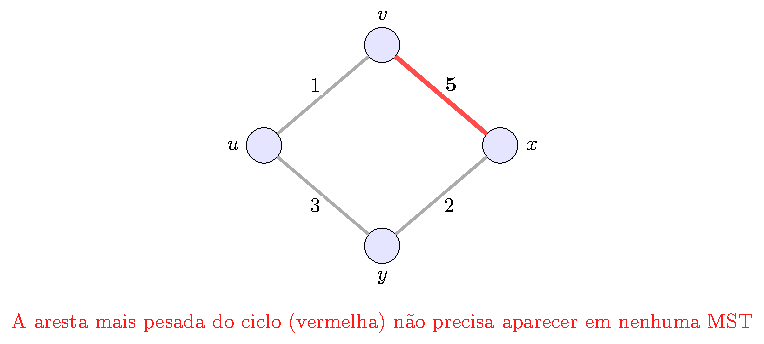
\includegraphics[width=0.9\linewidth]{figures/fig_mst_cycle_heavy.pdf}

    \caption{Princípio do ciclo: em qualquer ciclo, a aresta mais pesada (em vermelho) pode ser removida sem desconectar o grafo, reduzindo (ou não aumentando) o custo. Portanto, nenhuma MST contém a aresta mais pesada de um ciclo.}
    \label{fig:mst-cycle-heavy}\end{figure}

\end{itemize}

Assim o problema de encontrar uma árvore geradora mínima (MST) consiste em dado um grafo (não dirigido), conexo e ponderado \(G=(V,E)\) com pesos \(w:E\to\mathbb{R}\), queremos um subconjunto de arestas \(T\subseteq E\) que conecta todos os vértices sem ciclos (forma uma árvore) e minimiza \(\sum_{e\in T} w(e)\). 
Com base nos princípios acima, duas soluções gulosas são propostas: \textbf{Kruskal} e \textbf{Prim}.

\begin{itemize}\setlength{\itemsep}{2pt}
    \item \textbf{Kruskal}: ordena as arestas por peso e adiciona enquanto não formar ciclo; usa o princípio do ciclo para evitar carregar a aresta mais pesada de um ciclo.
    \item \textbf{Prim}: começa em um vértice e cresce a árvore; a cada passo escolhe a aresta mais leve que cruza o corte entre “dentro” e “fora” — aplicação direta do princípio do corte.
\end{itemize}


\begin{algobox}{Kruskal (MST, guloso por peso crescente)}{mst-kruskal}
Entrada: grafo não dirigido \(G=(V,E)\), pesos \(w\).
\begin{enumerate}\setlength{\itemsep}{2pt}
    \item Ordene as arestas por peso crescente.
    \item Inicialize um \emph{Union-Find}\footnote{Também conhecido como \emph{Disjoint Set Union} (DSU) ou \emph{estrutura de conjuntos disjuntos}. Mantém uma partição dinâmica dos vértices em componentes, oferecendo operações \texttt{find} (descobrir o representante do conjunto) e \texttt{union} (unir dois conjuntos). Com as heurísticas de \emph{união por rank/tamanho} e \emph{compressão de caminhos}, ambas operam em tempo amortizado \(\alpha(n)\) (a função inversa de Ackermann), efetivamente constante na prática. Em Kruskal, essa estrutura detecta ciclos rapidamente ao verificar se as pontas de uma aresta pertencem a componentes distintas.} com cada vértice em seu próprio conjunto; comece com \(T=\emptyset\).
    \item Para cada aresta \(e=\{u,v\}\) na ordem: se \(u\) e \(v\) estão em componentes diferentes, una as componentes e adicione \(e\) a \(T\).
    \item Pare quando \(|T|=|V|-1\). Devolva \(T\).
\end{enumerate}
\end{algobox}

\paragraph{}Kruskal é correto pelos princípios de corte e ciclo; com Union-Find eficiente, roda em \(O(m\log m)\) (ou \(O(m\log n)\)).

\begin{algobox}{Prim (MST, expansão por corte mínimo)}{mst-prim}
Entrada: grafo não dirigido \(G=(V,E)\), pesos \(w\), vértice inicial \(s\).
\begin{enumerate}\setlength{\itemsep}{2pt}
    \item Inicialize \(T=\{s\}\) e uma fila de prioridades\footnote{Estrutura que mantém elementos com chaves de prioridade e permite extrair rapidamente o de menor (ou maior) chave. Implementações típicas: \emph{heap} binário (\(\mathrm{push}/\mathrm{decrease\text{-}key}/\mathrm{pop}\) em \(O(\log n)\)), \emph{heap} de Fibonacci (\(\mathrm{decrease\text{-}key}\) amortizado \(O(1)\), \(\mathrm{pop}\) em \(O(\log n)\)), e, em grafos com pesos pequenos, fila bucket (Dial) com tempos quase-lineares. No Prim, a fila é chaveada pelo menor peso de aresta que conecta o vértice fora da árvore ao conjunto \(T\).} com as arestas que saem de \(T\), chaveando pelo menor peso.
    \item Enquanto \(|T|<|V|\): extraia a aresta mais leve \(\{u,v\}\) com \(u\in T\) e \(v\notin T\); adicione \(v\) e \(\{u,v\}\) à árvore; atualize as chaves das arestas que cruzam o novo corte.
    \item Devolva a árvore construída.
\end{enumerate}
\end{algobox}

\paragraph{}Prim também é correto pelo princípio do corte; com fila de prioridades binária, executa em \(O(m\log n)\) (ou em \(O(m+n\log n)\)); em grafos densos com \emph{heaps} de Fibonacci\footnote{\emph{Heaps} (montes) são implementações clássicas de filas de prioridades. O \textbf{heap binário} mantém uma árvore quase completa e executa \texttt{insert}/\texttt{extract-min}/\texttt{decrease-key} em \(O(\log n)\). Já o \textbf{heap de Fibonacci} é uma estrutura amortizada com \texttt{decrease-key} e \texttt{meld} (união) em \(O(1)\) amortizado e \texttt{extract-min} em \(O(\log n)\). Em algoritmos como Prim e Dijkstra, onde \texttt{decrease-key} é frequente, isso leva a \(O(m+n\log n)\). Apesar da melhor garantia assintótica, constantes e implementação mais simples fazem heaps binários (ou \emph{pairing heaps}) serem frequentemente competitivos na prática.}, pode-se obter \(O(m+n\log n)\) \cite{cormen2009,kleinberg2006,west2001introduction,diestel2017graph}.

\paragraph{}
Os algoritmos gulosos de MST são corretos em grafos não dirigidos, mas a passagem para dígrafos \emph{não} é direta. No caso dirigido, buscamos uma \textbf{r-arborescência de custo mínimo}: para cada \(v\neq r\), exatamente um arco entra em \(v\), e o conjunto deve ser acíclico e alcançável a partir de \(r\). Se imitarmos a receita de MST (escolher sempre o arco de entrada mais barato), aparecem \emph{ciclos dirigidos}, e não há um análogo imediato do “corte seguro”.

\paragraph{}
Duas abordagens clássicas contornam essas dificuldades: (i) \textbf{Chu–Liu/Edmonds}, que mantém \emph{custos reduzidos} (criando arcos de custo reduzido zero) e resolve conflitos por \emph{contração de ciclos}; e (ii) o procedimento em duas fases de \textbf{Frank}, que parte de uma arborescência qualquer e a refina via ajustes de custos e trocas de arcos. Em ambos os casos, escolhas locais são acopladas a um mecanismo global de consistência, garantindo otimalidade no caso dirigido \cite{schrijver2003comb}.

\subsubsection{A busca em digrafos}

\paragraph{}
O primeiro avanço significativo na busca por arborescências de custo mínimo em dígrafos foi feito por Y. Chu e T. Liu em 1965, que propuseram um algoritmo para encontrar a arborescência de custo mínimo em um dígrafo. Esse algoritmo foi posteriormente aprimorado por Jack Edmonds em 1967, que introduziu o conceito de custos reduzidos e a técnica de contração de ciclos, tornando o algoritmo mais eficiente e robusto.

\paragraph{}
Desde então, a pesquisa nessa área tem se concentrado em melhorar a eficiência dos algoritmos existentes, bem como em explorar novas técnicas e abordagens para lidar com diferentes tipos de dígrafos e restrições adicionais. A contribuição de András Frank, que propôs um procedimento em duas fases para encontrar arborescências de custo mínimo, é um exemplo notável dessa evolução contínua.

\subsection{Os meios para um fim}

\paragraph{}
Maquiável é conhecido por uma de suas citações: "Os fins justificam os meios". Essa frase ficou famosa, porque tem uma interpretação polêmica: em certas circunstâncias, qualquer ação pode ser justificada se o resultado final for considerado positivo ou benéfico. Muitos, não concordam com essa visão, argumentando que os meios também importam e que ações imorais não podem ser justificadas por bons resultados.

\paragraph{}
Por um lado, na matemática essa frase pode ser validada quando falamos em duas formas distintas de construir algoritmos: por \emph{iteratividade} ou \emph{recursividade}.

\paragraph{Iteratividade}
\paragraph{}
Muitos algoritmos — incluindo os gulosos — são construídos por \emph{iteração}: repetimos um bloco de instruções enquanto uma condição não é satisfeita. Para projetar e analisar laços com clareza, três ideias são centrais:

\begin{itemize}\setlength{\itemsep}{2pt}
    \item \textbf{Invariante de laço}: uma propriedade que é verdadeira antes do laço e permanece verdadeira a cada iteração. Ela explica \emph{o que} está sendo mantido correto durante a construção.
    \item \textbf{Variante (medida de progresso)}: uma quantidade que melhora estritamente a cada iteração (ex.: aumenta $|T|$, diminui $|V|$, reduz um potencial). Garante \emph{terminação}.
    \item \textbf{Critério de parada e pós-condição}: quando o laço termina, o invariante implica a especificação desejada.
\end{itemize}

\paragraph{}
	\textit{Na prática.} Em \textbf{Kruskal}, o invariante é “$T$ é uma floresta acíclica e cada componente foi conectado por arestas seguras”; a variante é $|T|$, que cresce até $|V|-1$. Em \textbf{Prim}, “$T$ conecta um conjunto de vértices e as chaves refletem o menor corte atual”; a variante é o tamanho de $T$. Muitas análises usam \emph{custo por iteração} ou \emph{análise amortizada}\footnote{A análise amortizada distribui o custo de operações caras sobre uma sequência, garantindo um custo médio por operação (ex.: \texttt{decrease-key} em heaps de Fibonacci).} para capturar o desempenho agregado.

\paragraph{Recursividade}
\paragraph{}
Recursão resolve instâncias grandes chamando o próprio algoritmo em subinstâncias menores. Um projeto claro inclui:

\begin{itemize}\setlength{\itemsep}{2pt}
    \item \textbf{Casos base}: instâncias mínimas resolvidas diretamente.
    \item \textbf{Passo recursivo}: como decompor e combinar soluções dos subproblemas.
    \item \textbf{Medida decrescente}: uma grandeza que estritamente diminui a cada chamada (ex.: número de vértices após contração), assegurando terminção.
    \item \textbf{Corretude por indução}: assumimos corretas as chamadas recursivas (hipótese indutiva) e provamos que a combinação produz uma solução correta.
    \item \textbf{Custo por recorrência}: tempo expresso por $T(n)$ e resolvido por \emph{árvore de recursão} ou Teorema Mestre\footnote{Esboço: quando $T(n)=a\,T(n/b)+f(n)$, com $a\ge 1$, $b>1$, comparamos $f(n)$ a $n^{\log_b a}$. Não é necessário aqui, mas a técnica guia estimativas assintóticas.}.
\end{itemize}

\paragraph{}
	\textit{Na prática.} Em \textbf{Chu–Liu/Edmonds}, o passo recursivo contrai um ciclo dirigido e ajusta custos; a medida decrescente é $|V|$ (a cada contração reduzimos o número de vértices do problema), e a expansão final preserva otimalidade. No procedimento em duas fases de \textbf{Frank}, a primeira fase produz uma arborescência inicial; a segunda aplica \emph{refinamentos iterativos} guiados por custos reduzidos — um exemplo de mistura entre recursão estrutural e iteração local.

\paragraph{}
Para ilustrar, resolvemos o mesmo problema — calcular o fatorial \(n!\) — de forma \emph{iterativa} e \emph{recursiva}.

\begin{algobox}{Fatorial (iterativo)}{fatorial-iterativo}
Entrada: inteiro \(n\ge 0\)
\begin{enumerate}\setlength{\itemsep}{2pt}
    \item Se \(n=0\), devolva \(1\).
    \item Defina \(r\leftarrow 1\).
    \item Para \(i\) de \(1\) até \(n\): \(r\leftarrow r\cdot i\).
    \item Devolva \(r\).
\end{enumerate}
\end{algobox}

\begin{algobox}{Fatorial (recursivo)}{fatorial-recursivo}
Entrada: inteiro \(n\ge 0\)
\begin{enumerate}\setlength{\itemsep}{2pt}
    \item Se \(n\le 1\), devolva \(1\). \hfill (caso base)
    \item Caso contrário, devolva \(n\cdot \textsc{Fatorial}(n-1)\). \hfill (passo recursivo)
\end{enumerate}
\end{algobox}

\paragraph{}
Ambas as versões computam a mesma função. A iterativa evidencia a \emph{variante} (o contador \(i\)) e um \emph{invariante} simples (\(r= i!\) ao fim da iteração \(i\)); a recursiva explicita o \emph{caso base} e o \emph{passo indutivo}, e corresponde, operacionalmente, a empilhar chamadas com parâmetros decrescentes até \(n=1\).    

\paragraph{}
Existe inclusive uma prova matemática\footnote{Em modelos padrão de computação (máquinas de Turing, RAM), \emph{iteração} e \emph{recursão} têm o mesmo poder expressivo: laços podem ser reescritos como recursão (sobre um contador/estado) e chamadas recursivas podem ser eliminadas por uma simulação explícita da pilha (iteração com uma estrutura \textit{stack}). Demonstrações e variantes aparecem em textos clássicos de teoria da computação e projeto de algoritmos; ver, por exemplo, \cite{cormen2009} (eliminação de recursão via pilha explícita). Aqui registramos apenas a equivalência conceitual, sem apresentá-la.} que diz que qualquer algoritmo iterativo pode ser reescrito de forma recursiva, e vice-versa. Ou seja, \emph{os fins justificam os meios}: a escolha entre iteração e recursão é muitas vezes uma questão de preferência ou conveniência, já que ambos podem alcançar o mesmo objetivo. Porém, algoritmos recursivos podem ser mais elegantes e fáceis de entender, enquanto algoritmos iterativos podem ser mais eficientes em termos de uso de memória (evitando a sobrecarga da pilha de chamadas). Ou seja, os meios também importam. E os trabalhos de Chu–Liu/Edmonds e Frank ilustram bem essa tensão:
\begin{itemize}\setlength{\itemsep}{2pt}
    \item \textbf{Chu–Liu/Edmonds} é um algoritmo recursivo que contrai ciclos e resolve o problema em subinstâncias menores, usando custos reduzidos para manter a otimalidade.
    \item O procedimento em \textbf{Frank} é iterativo, começando com uma arborescência qualquer e refinando-a por trocas locais guiadas por custos reduzidos, até alcançar a otimalidade.
\end{itemize}
Ambos os algoritmos são corretos e eficientes, mas adotam meios diferentes para alcançar o mesmo fim: encontrar uma r-arborescência de custo mínimo em um dígrafo ponderado.

\paragraph{}
Antes de entrar nos detalhes, faremos uma breve revisão dos conceitos e técnicas que utilizaremos adiante, para uniformizar a notação e tornar a leitura mais fluida.

\paragraph{Revisão: conceitos fundamentais e técnicas}

\paragraph{}
Antes de mergulharmos nos algoritmos específicos, é importante revisitar alguns conceitos fundamentais que serão cruciais para nossa compreensão:

\paragraph{Conceitos Fundamentais:}
\begin{itemize}\setlength{\itemsep}{2pt}
    \item \textbf{Dígrafo}: um grafo direcionado onde os arcos têm uma direção específica, indo de um vértice a outro.
    \item \textbf{Arborescência}: uma árvore direcionada onde todos os caminhos partem de um vértice raiz e alcançam todos os outros vértices.
    \item \textbf{Custo dos Arcos}: cada arco em um dígrafo pode ter um custo associado, representando, por exemplo, o custo de transporte ou a distância.
    \item \textbf{r-Arborescência de Custo Mínimo}: uma arborescência enraizada em um vértice \(r\) que minimiza a soma dos custos dos arcos que a compõem.
    \item \textbf{Cortes e Conectividade}: a importância dos cortes em dígrafos para garantir a conectividade e a existência de arborescências.
    \item \textbf{Condicionalidade de Fulkerson}: as condições necessárias e suficientes para a existência de uma r-arborescência de custo mínimo.
\end{itemize}

\paragraph{Técnicas e Abordagens:}
\paragraph{}
Para encontrar r-arborescências de custo mínimo, utilizaremos algumas técnicas e abordagens específicas:
\begin{itemize}\setlength{\itemsep}{2pt}
    \item \textbf{Normalização de Custos}: ajustaremos os custos dos arcos para facilitar a identificação de arcos de custo reduzido zero.
    \item \textbf{Contração de Ciclos}: quando formos encontrar ciclos de arcos de custo reduzido zero, os contrairemos para simplificar o dígrafo.
    \item \textbf{Custos Reduzidos}: utilizaremos custos reduzidos para identificar arcos que podem ser incluídos na arborescência sem aumentar o custo total.
    \item \textbf{Estratégias Gulosas}: aplicaremos estratégias gulosas para selecionar arcos de forma eficiente, garantindo que cada escolha local contribua para a solução global ótima.
    \item \textbf{Recursão e Expansão}: usaremos recursão para resolver subproblemas em dígrafos contraídos e expandiremos as soluções para o dígrafo original.
    \item \textbf{Análise de Complexidade}: avaliaremos a eficiência dos algoritmos em termos de tempo e espaço, garantindo que sejam viáveis para grandes dígrafos.
    \item \textbf{Provas de Corretude}: forneceremos argumentos formais para garantir que os algoritmos realmente produzem a r-arborescência de custo mínimo.
\end{itemize}

\paragraph{}
No capítulo seguinte, detalharemos o algoritmo de Chu–Liu/Edmonds, bem como os detalhes da implementação em Python; o subsequente será dedicado ao procedimento em duas fases de Frank e à respectiva implementação.

\section{Algoritmo de Chu–Liu/Edmonds}

\paragraph{}
O algoritmo de Chu–Liu/Edmonds é um método clássico para encontrar uma r-arborescência de custo mínimo em um dígrafo ponderado. Ele combina estratégias gulosas com técnicas de normalização de custos e contração de ciclos para garantir a otimalidade da solução.

\paragraph{}
Se tentarmos copiar a receita das MSTs — dar a cada vértice \(v\neq r\) o arco de entrada mais barato — corremos o risco de fechar um \emph{ciclo dirigido} que não chega à raiz \(r\). 

\paragraph{}
Por que isso é proibido? Em uma r‑arborescência cada \(v\neq r\) deve ter exatamente um arco de entrada e \(r\) tem grau de entrada zero. Se houvesse um ciclo dirigido \(C\), todos os vértices de \(C\) já receberiam seu único arco de entrada de dentro do próprio \(C\), logo nenhum arco entraria em \(C\) a partir de \(V\setminus C\) (o corte \(\delta^-(C)\) ficaria vazio). Como \(r\notin C\), não existe caminho de \(r\) para os vértices de \(C\), contrariando a alcançabilidade exigida. Portanto, ciclos dirigidos são incompatíveis com a estrutura de r‑arborescência.

\paragraph{}
Dessa forma, o desafio é duplo: preservar a informação local de “mais barato por vértice” (que é valiosa) e, ao mesmo tempo, impedir que essas escolhas locais se combinem em ciclos. 

\paragraph{}
Uma maneira direta de enxergar isso é com um microexemplo: tome três vértices \(a,b,c\) (todos fora de \(r\)). Se o arco mais barato que entra em \(b\) vem de \(a\), o de \(c\) vem de \(b\) e o de \(a\) vem de \(c\), então as escolhas “mais baratas” formam o ciclo \(a\to b\to c\to a\). Note que, entre essas escolhas locais, nenhum deles recebe o arco vindo de \(r\) (mesmo que existam \(r\to a\), \(r\to b\), \(r\to c\) mais caros); ficamos presos dentro do ciclo e não alcançamos a raiz. É exatamente esse impasse que o algoritmo resolve ao zerar custos por vértice e contrair ciclos, deixando para decidir qual arco interno remover apenas na expansão.


\begin{figure}[H]
    \centering
    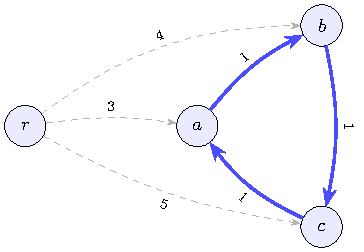
\includegraphics[width=0.9\linewidth]{figures/fig_chu_liu_cycle_micro.pdf}

    \caption{Ciclo gerado pelas escolhas locais “mais baratas por vértice”. Os arcos grossos (custo 1) entram em \(a,b,c\) e formam \(a\to b\to c\to a\). Os arcos tracejados partindo de \(r\) existem, mas são mais caros e por isso não são escolhidos pelo critério local.}
    \label{fig:chu-liu-cycle-micro}\end{figure}


\paragraph{}
Partindo desse cenário, a ideia é \emph{normalizar os custos por vértice}: para cada \(v\neq r\), “descontamos” de todo arco que entra em \(v\) o menor custo que chega a \(v\). Após esse ajuste (custos reduzidos), cada \(v\neq r\) passa a ter ao menos um arco de custo reduzido zero entrando. Se os arcos de custo zero forem acíclicos, já temos a r‑arborescência. Se formarem um ciclo \(C\), isso indica que, dentro de \(C\), todos os vértices atingiram seus mínimos locais; então \emph{contraímos} \(C\) em um \textbf{supervértice} \(x_C\) e repetimos o processo no grafo menor. Ao final, \emph{expandimos} as contrações e, em cada ciclo expandido, removemos exatamente um arco para manter grau de entrada 1 e a aciclicidade global.

\paragraph{Supervértices e contração de ciclos}

\paragraph{}
Dado um subconjunto \(C\subseteq V\) que forma um ciclo dirigido, a \emph{contração de \(C\)} substitui todos os vértices de \(C\) por um único vértice \(x_C\) - \textbf{o supervértice}. Todo arco com exatamente uma ponta em \(C\) passa a ser incidente a \(x_C\):
\begin{itemize}\setlength{\itemsep}{2pt}
    \item arcos \((u,w)\) com \(u\notin C\), \(w\in C\) tornam-se \((u, x_C)\);
    \item arcos \((w,v)\) com \(w\in C\), \(v\notin C\) tornam-se \((x_C, v)\);
    \item arcos com as duas pontas em \(C\) tornam-se laços em \(x_C\) e são descartados.
\end{itemize}
Quando trabalhamos com \emph{custos reduzidos}, ajustamos em particular os arcos que \emph{entram} em \(C\) para preservar a comparação relativa: para um arco \((u,w)\) com \(w\in C\), definimos \(c'(u,x_C) = c(u,w) - c(a_w)\), onde \(a_w\) é o arco mais barato que entra em \(w\). Essa normalização garante que, ao resolver no grafo contraído, decisões ótimas podem ser traduzidas de volta na etapa de expansão.


\begin{figure}[H]
    \centering
    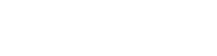
\includegraphics[width=0.9\linewidth]{figures/fig_chu_liu_reduced_cost.pdf}

    \caption{Ajuste de custo reduzido para um arco \emph{entrando}: ao contrair um ciclo $C$, o arco $(u,w)$ que entra em $w\in C$ passa a $(u,x_C)$ com custo reduzido $c'(u,x_C)=c(u,w)-c(a_w)$, onde $a_w$ é o arco mais barato que entra em $w$.}
    \label{fig:chu-liu-reduced-cost}
    \end{figure}


Para cada arco \((u,w)\) com \(w\in C\), ajustamos o custo reduzido para \(c'(u,x_C)=c(u,w)-c(a_w)\), onde \(a_w\) é o arco mais barato que entra em \(w\). No exemplo da Figura \ref{fig:chu-liu-reduced-cost}, o arco \((u,b)\) com custo \(7\) torna-se \((u,x_C)\) com custo reduzido \(7-5=2\), já que \(a_b=(a\to b)\) tem custo \(5\). Arcos que saem de \(C\) ou laços internos não são ajustados.

\subsection{Descrição do algoritmo}

\paragraph{}
Em computação falamos em linguagem de alto nível quando uma linguagem de programação é próxima da linguagem humana, com abstrações que facilitam o entendimento. Em contraste, linguagens de baixo nível são mais próximas do código de máquina, exigindo detalhes explícitos. 

\paragraph{}
Podemos falar também em visão operacional de alto nível quando descrevemos um algoritmo focando na lógica e nos passos principais, sem entrar em detalhes de implementação específicos.

\paragraph{}
Aqui, apresentamos o algoritmo de Chu–Liu/Edmonds em uma visão operacional de alto nível, focando na lógica e nos passos principais, sem entrar em detalhes de implementação específicos. E dedicaremos a próxima subseção apenas para discutir detalhes práticos de implementação.

\subsection{Descrição do Algoritmo}
\paragraph{}
Denotamos por \(A'\) o conjunto de arcos escolhidos na construção da r-arborescência. 

\paragraph{}
Construa \(A'\) escolhendo, para cada \(v\neq r\), um arco de menor custo que \emph{entra} em \(v\). Se \((V,A')\) é acíclico, então, pela caracterização de arborescências (grau de entrada 1 para todo \(v\neq r\) e ausência de ciclos), \(A'\) já é uma r‑arborescência; e é \emph{ótima}, pois realizamos o menor custo de entrada em cada vértice e nenhuma troca pode reduzir o custo mantendo as restrições \cite[Sec.~4.9]{kleinberg2006}. 

\paragraph{}
Se \(A'\) contiver um ciclo dirigido \(C\) (que não inclui \(r\)), normalizamos os custos de entrada (custos reduzidos) e \emph{contraímos} \(C\) em um supervértice \(x_C\), ajustando apenas arcos que \emph{entram} em \(C\) por \(c'(u,x_C)=c(u,w)-c(a_w)\). 

\paragraph{}
Resolvemos recursivamente no grafo contraído. As arborescências do grafo contraído correspondem, em bijeção, às arborescências do grafo original com exatamente um arco entrando em \(C\); como os arcos de \(C\) têm custo reduzido zero, os custos são preservados na ida e na volta. 


\begin{figure}[H]
    \centering
    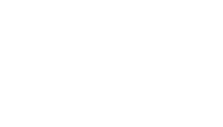
\includegraphics[width=0.9\linewidth]{figures/fig_chu_liu_bijection.pdf}

    \caption{Bijeção entre arborescências após contração e no grafo original. (a) No grafo contraído, toda arborescência seleciona exatamente um arco que entra no supervértice $x_C$. (b) Ao expandir $C$, escolhe-se o arco correspondente \((u,w)\) que entra em algum $w\in C$ e mantêm-se os arcos internos de custo reduzido zero, removendo exatamente um para quebrar o ciclo. Como $c'(u,x_C)=c(u,w)-c(a_w)$ e os arcos internos têm custo reduzido zero, o custo total é preservado na ida e na volta.}
    \label{fig:chu-liu-bijection}\end{figure}


\paragraph{}
A Figura \ref{fig:chu-liu-bijection} ilustra a bijeção entre arborescências no grafo contraído e no grafo original, destacando a preservação de custos e a manutenção das propriedades estruturais necessárias.

\paragraph{}
Na expansão, reintroduzimos \(C\) e removemos exatamente um arco interno para manter grau de entrada 1 e aciclicidade global \cite{schrijver2003comb,kleinberg2006}.


\begin{figure}[H]
    \centering
    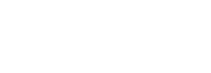
\includegraphics[width=0.9\linewidth]{figures/fig_chu_liu_reexpansion.pdf}

    \caption{Reexpansão de $C$. (a) No grafo contraído, seleciona-se um único arco que entra em $x_C$. (b) Ao expandir, $x_C$ é substituído pelo ciclo $C$ e o arco selecionado passa a entrar em algum $w\in C$. (c) Remove-se exatamente um arco interno de $C$ para eliminar o ciclo, preservando conectividade a partir de $r$ e o custo total, pois os arcos internos têm custo reduzido zero.}
    \label{fig:chu-liu-reexpansion}\end{figure}


\paragraph{}
A Figura \ref{fig:chu-liu-reexpansion} detalha o processo de expansão e remoção de um arco interno para quebrar o ciclo, garantindo que a estrutura de r-arborescência seja mantida.

\paragraph{}
Abaixo, temos a descrição formal do algoritmo.
\paragraph{}
\begin{algobox}{Chu–Liu/Edmonds (visão operacional)}{chu-liu-edmonds}
Entrada: dígrafo \(D=(V,A)\), custos \(c:A\to\mathbb{R}_{\ge 0}\), raiz \(r\).\footnote{Se algum \(v\neq r\) não possui arco de entrada, não existe r‑arborescência.}
\begin{enumerate}\setlength{\itemsep}{2pt}
    \item Para cada \(v\neq r\), escolha \(a_v\in\operatorname*{argmin}_{(u,v)\in A} c(u,v)\). Defina \(y(v):=c(a_v)\) e \(F^*:=\{a_v: v\neq r\}.\)
    \item Se \((V,F^*)\) é acíclico, devolva \(F^*\). Por \cite[Obs.~4.36]{kleinberg2006}, trata‑se de uma r‑arborescência de custo mínimo.
    \item Caso contrário, seja \(C\) um ciclo dirigido de \(F^*\) (com \(r\notin C\)). \textbf{Contração:} contraia \(C\) em um supervértice \(x_C\) e defina custos \(c'\) por
    \begin{align*}
        c'(u,x_C) &:= c(u,w) - y(w) = c(u,w) - c(a_w) && \text{para } u\notin C,\ w\in C, \\
        c'(x_C,v) &:= c(w,v) && \text{para } w\in C,\ v\notin C,
    \end{align*}
    descartando laços em \(x_C\) e permitindo paralelos. Denote o dígrafo contraído por \(D'=(V',A')\).
    \item \textbf{Recursão:} compute uma r‑arborescência ótima \(T'\) de \(D'\) com custos \(c'\).
    \item \textbf{Expansão:} seja \((u,x_C)\in T'\) o único arco que entra em \(x_C\). No grafo original, ele corresponde a \((u,w)\) com \(w\in C\). Forme
    \[
        T := \bigl(T'\setminus\{\text{arcos incidentes a } x_C\}\bigr)\ \cup\ \{(u,w)\}\ \cup\ \bigl((F^*\cap A(C))\setminus\{a_w\}\bigr).
    \]
    Então \(T\) tem grau de entrada 1 em cada \(v\neq r\), é acíclico e tem o mesmo custo de \(T'\); logo, é uma r‑arborescência ótima de \(D\) \cite[Sec.~4.9]{kleinberg2006,schrijver2003comb}.
\end{enumerate}
\end{algobox}

\subsubsection{Corretude}
\paragraph{}
A corretude do algoritmo de Chu–Liu/Edmonds baseia-se em três pilares principais:
\begin{enumerate}\setlength{\itemsep}{2pt}
    \item \emph{Normalização por custos reduzidos:} para cada \(v\neq r\), defina \(y(v):=\min\{c(u,v):(u,v)\in A\}\) e \(c'(u,v):=c(u,v)-y(v)\). Para qualquer r‑arborescência \(T\), vale
    \[
        \sum_{a\in T} c'(a) \,=\, \sum_{a\in T} c(a) \, - \, \sum_{v\neq r} y(v),
    \]
    pois há exatamente um arco de \(T\) entrando em cada \(v\neq r\). O termo \(\sum_{v\neq r} y(v)\) é constante (independe de \(T\)); assim, minimizar \(\sum c\) equivale a minimizar \(\sum c'\) \cite[Obs.~4.37]{kleinberg2006}. Em particular, os arcos \(a_v\) de menor custo que entram em \(v\) têm custo reduzido zero e formam \(F^*\).
    \item \emph{Caso acíclico:} se \((V,F^*)\) é acíclico, então já é uma r‑arborescência e, por realizar o mínimo custo de entrada em cada \(v\neq r\), é ótima \cite[Obs.~4.36]{kleinberg2006}.
    \item \emph{Caso com ciclo (contração/expansão):} se \(F^*\) contém um ciclo dirigido \(C\), todos os seus arcos têm custo reduzido zero. 
    \paragraph{}
    Contraia \(C\) em \(x_C\) e ajuste apenas arcos que \emph{entram} em \(C\): \(c'(u,x_C):=c(u,w)-y(w)=c(u,w)-c(a_w)\). 
    \paragraph{}
    Resolva o problema no grafo contraído \(D'\), obtendo uma r‑arborescência ótima \(T'\) sob \(c'\). Na expansão, substitua o arco \((u,x_C)\in T'\) pelo correspondente \((u,w)\) (com \(w\in C\)) e remova \(a_w\) de \(C\). 
    \paragraph{}
    Como os arcos de \(C\) têm custo reduzido zero e \(c'(u,x_C)=c(u,w)-y(w)\), a soma dos custos reduzidos é preservada na ida e na volta; logo, \(T'\) ótimo em \(D'\) mapeia para \(T\) ótimo em \(D\) para \(c'\). Pela equivalência entre \(c\) e \(c'\), \(T\) também é ótimo para \(c\). Repetindo o argumento a cada contração, obtemos a corretude por indução \cite[Sec.~4.9]{kleinberg2006,schrijver2003comb}.
\end{enumerate}
Em termos intuitivos, \(y\) funciona como um potencial nos vértices: torna “apertados” (custo reduzido zero) os candidatos corretos; ciclos de arcos apertados podem ser contraídos sem perder otimalidade.

\subsubsection{Complexidade}
\paragraph{}
Na implementação direta, selecionar os \(a_v\), detectar/contrair ciclos e atualizar estruturas custa \(O(m)\) por nível; como o número de vértices decresce a cada contração, temos no máximo \(O(n)\) níveis e tempo total \(O(mn)\), com \(n=|V|\), \(m=|A|\).


\paragraph{}
O uso de memória é \(O(m+n)\), incluindo mapeamentos de contração/expansão e as filas de prioridade dos arcos de entrada. A implementação a seguir adota a versão \(O(mn)\) por simplicidade e está disponível no repositório do projeto (\url{https://github.com/lorenypsum/GraphVisualizer}).

\subsection{Implementação em Python}

\paragraph{}
Esta seção apresenta uma implementação em Python do algoritmo de Chu–Liu/Edmonds, baseada no código do trabalho. A arquitetura segue os passos teóricos:

\begin{itemize}\setlength{\itemsep}{2pt}
    \item seleção dos arcos de menor custo que entram em cada vértice (formação de \(F^*\));
    \item verificação de aciclicidade (se acíclico, retorno imediato);
    \item se houver ciclo, normalização dos custos por vértice (custos reduzidos);
    \item construção do grafo funcional \(F^*\) com arcos de custo reduzido zero;
    \item detecção de ciclo em \(F^*\);
    \item contração do ciclo em um supervértice, com ajuste de custos;
    \item recursão no grafo contraído;
    \item expansão do ciclo e remoção de um arco interno para quebrar o ciclo.
    \item retorno da r‑arborescência ótima.
\end{itemize}

\paragraph{Especificação da interface (entradas, saídas e hipóteses)}

\begin{itemize}\setlength{\itemsep}{2pt}
    \item \textbf{Entrada:} dígrafo ponderado \(D=(V,A)\), custos \(c:A\to\mathbb{R}\), raiz \(r\in V\).
    \item \textbf{Hipóteses:}
        \begin{itemize}\setlength{\itemsep}{2pt}
            \item \(D\) é representado como um objeto \texttt{networkx.DiGraph}, com pesos armazenados no atributo de arestas \texttt{'w'}.
            \item \(D\) é conexo a partir de \(r\):
            \item (i) todo \(v\neq r\) é alcançável a partir de \(r\) (caso contrário, não há r‑arborescência); (ii) para todo subconjunto não vazio \(X\subseteq V\setminus\{r\}\), existe ao menos um arco que entra em \(X\) (\(\delta^-(X)\neq\emptyset\); condições clássicas de existência \`a la Edmonds \cite{schrijver2003comb}).
            \item Os custos são não negativos: \(c(a)\ge 0\) para todo \(a\in A\).
        \end{itemize}
    \item \textbf{Saída:} conjunto \(A^*\subseteq A\) com \(|A^*|=|V|-1\), tal que cada \(v\neq r\) tem grau de entrada 1, todos os vértices são alcançáveis a partir de \(r\) e \(\sum_{a\in A^*} c(a)\) é mínimo.
    \item \textbf{Convenções:} arcos paralelos (múltiplos arcos entre o mesmo par de vértices) são permitidos após contrações; laços (self‑loops) são descartados.
\end{itemize}


\subsubsection{Funções principais}

\paragraph{}
O código a seguir implementa o algoritmo de Chu–Liu/Edmonds em Python, utilizando a biblioteca NetworkX para manipulação de grafos. A implementação segue a estrutura descrita na seção anterior, com funções auxiliares para cada etapa do algoritmo.

\paragraph{}
A seguir, detalhamos as implementações das funções auxiliares e as principais, começando pela normalização dos custos por vértice.

\paragraph{Normalização por vértice:}
para um vértice alvo $v$, a função normaliza\footnote{Aqui, “normalizar” significa subtrair do peso de cada aresta que entra em $v$ o menor peso de entrada de $v$ (custos reduzidos), preservando a ordem relativa entre as entradas; assim, ao menos uma entrada em $v$ passa a ter custo 0, sem afetar a comparação entre soluções.} os custos das arestas que \emph{entram} em $v$: calcula $y(v)=\min\{w(u,v)\}$ e 
substitui cada peso $w(u,v)$ por $w(u,v)-y(v)$. 

\paragraph{}
Com isso, ao menos uma entrada em $v$ passa a ter custo reduzido zero e a ordem relativa entre as entradas é preservada. A função modifica o grafo \emph{in-place}\footnote{No jargão de programação, significa “no próprio lugar”: a estrutura de dados original é alterada diretamente, sem criar uma cópia. Isso economiza memória e tempo, mas introduz efeitos colaterais — outras referências ao mesmo objeto verão as mudanças.}, ou seja, sem criar uma cópia. 

\paragraph{}
A função executa em $O(\deg^-(v))$. Pois, dado o vértice $v$, obtemos suas arestas de entrada em $O(\deg^-(v))$; calcular o mínimo e ajustar os pesos também leva $O(\deg^-(v))$.

\begin{pybox}{Normalização por vértice: custos reduzidos}
def normalize_incoming_edge_weights(D: nx.DiGraph, node: str, lang="pt"):
    """
    Altera os pesos das arestas que entram em `node`
    subtraindo de cada uma o menor peso de entrada no grafo D.

    Parâmetros:
        - D: Um grafo direcionado (networkx.DiGraph)
        - node: O vértice alvo cujas arestas de entrada serão ajustadas
        - lang: Idioma das mensagens de erro ("en" para inglês, "pt" para português)

    Retorno:
        - Nada (o grafo D é modificado no próprio lugar — in-place)
    """

    if lang == "en":
        assert (
            node in D
        ), f"\nnormalize_incoming_edge_weights: The vertex '{node}' does not exist in the graph."
    elif lang == "pt":
        assert (
            node in D
        ), f"\nnormalize_incoming_edge_weights: O vértice '{node}' não existe no grafo."

    # Get the incoming edges of the node with their weights
    predecessors = list(D.in_edges(node, data="w"))

    if not predecessors:
        return

    # Calculate the minimum weight among the incoming edges
    yv = min((w for _, _, w in predecessors))

    # Subtract Yv from each incoming edge
    for u, _, _ in predecessors:
        D[u][node]["w"] -= yv
\end{pybox}

\paragraph{Construção de \(F^*\):}
a função constrói o subdígrafo \(F^*\) selecionando, para cada vértice \(v\neq r_0\), uma única aresta de menor custo que entra em \(v\) (isto é, um \(\operatorname*{argmin}_{(u,v)\in A} w(u,v)\)). 

\paragraph{}
Se os custos já foram normalizados por vértice, o arco escolhido tem custo reduzido zero; caso contrário, ele devolve None. O resultado é um dígrafo com exatamente uma aresta entrando em cada \(v\neq r_0\) e nenhuma aresta entrando em \(r_0\). A função executa em \(O(m)\), onde \(m\) é o número de arestas. 

\paragraph{}
Isso ocorre porque a função itera sobre todos os vértices do grafo e, para cada vértice, verifica suas arestas de entrada para encontrar a de menor peso. Como cada aresta é considerada no máximo uma vez durante essa iteração, o tempo total é proporcional ao número de arestas, ou seja, \(O(m)\). A função não modifica o grafo original, mas cria um novo grafo direcionado \(F^*\).

\begin{pybox}{Construção de $F^*$}
def get_Fstar(D: nx.DiGraph, r0: str, lang="pt"):
    """
    Constrói o subgrafo funcional F* a partir do grafo D e da raiz r0.
    Retorna um grafo direcionado F_star com exatamente uma aresta de entrada
    para cada v != r0 e nenhuma aresta entrando em r0.

    Parâmetros:
        - D: Um grafo direcionado (networkx.DiGraph)
        - r0: Vértice raiz (rótulo)
        - lang: Idioma das mensagens de erro ("en" para inglês, "pt" para português)

    Retorno:
        - F_star: Um grafo direcionado (networkx.DiGraph) que representa F*
    """

    if lang == "en":
        assert (
            r0 in D
        ), f"\nget_Fstar: The root vertex '{r0}' does not exist in the graph."
    elif lang == "pt":
        assert r0 in D, f"\nget_Fstar: O vértice raiz '{r0}' não existe no grafo."

    # Create an empty directed graph for F_star
    F_star = nx.DiGraph()

    for v in D.nodes():
        if v != r0:
            in_edges = list(D.in_edges(v, data="w"))
            if not in_edges:
                continue  # No edges entering v
            u = next((u for u, _, w in in_edges if w == 0), None)
            if u:
                F_star.add_edge(u, v, w=0)
    return F_star
\end{pybox}

\paragraph{Detecção de ciclo:}
a função detecta um ciclo dirigido em \(F^*\) (se existir) e retorna um subgrafo contendo o ciclo. Caso contrário, retorna None. A função utiliza a função \texttt{find\_cycle} do NetworkX, que implementa um algoritmo eficiente de detecção de ciclos. 

\paragraph{}
A função executa em \(O(m)\). Isso ocorre porque a função \texttt{find\_cycle} do NetworkX utiliza uma abordagem baseada em busca em profundidade (DFS) para detectar ciclos em grafos direcionados. 

\paragraph{}
A complexidade dessa abordagem é linear em relação ao número de vértices e arestas do grafo, ou seja, \(O(m)\), onde \(m\) é o número de arestas. A função não modifica o grafo original, mas cria um subgrafo contendo apenas os vértices e arestas que fazem parte do ciclo detectado.

\begin{pybox}{Detecção de ciclo dirigido em $F^*$}
def find_cycle(F_star: nx.DiGraph):
    """
    Encontra um ciclo dirigido no grafo.
    Retorna um subgrafo contendo o ciclo, ou None caso não exista.

    Parâmetros:
        - F_star: Um grafo direcionado (networkx.DiGraph)

    Retorno:
        - Um grafo direcionado (networkx.DiGraph) representando o ciclo, ou None se nenhum ciclo for encontrado.
    """

    try:
        nodes_in_cycle = set()
        # Extract nodes involved in the cycle
        for u, v, _ in nx.find_cycle(F_star, orientation="original"):
            nodes_in_cycle.update([u, v])
        # Create a subgraph containing only the cycle
        return F_star.subgraph(nodes_in_cycle).copy()

    except nx.NetworkXNoCycle:
        return None
\end{pybox}

\paragraph{Contração de ciclo:}
a função contrai um ciclo dirigido simples \(C\) em um \textbf{supervértice} \(x_C\), redirecionando arcos incidentes a \(C\) e ajustando custos de acordo com a regra de \emph{custos reduzidos}. O grafo é modificado \emph{in-place} e a rotina devolve dicionários auxiliares para permitir a \emph{reexpansão} correta do ciclo.

\paragraph{} Em alto nível, a rotina:
\begin{itemize}\setlength{\itemsep}{2pt}
    \item \textbf{Pré-condições:} 
    \paragraph{}
    (i) \(C\) induz um ciclo dirigido em \(D\); 
    \paragraph{}
    (ii) a raiz \(r_0\) não pertence a \(C\); 
    \paragraph{}
    (iii) o rótulo \(\texttt{label}\) não existe como vértice em \(D\) (é o nome de \(x_C\)).
    \item \textbf{Ajuste de custos (entradas em \(C\)):} para cada arco \((u,w)\) com \(u\notin C\), \(w\in C\), cria \((u, x_C)\) com custo \(c'(u,x_C) := c(u,w) - y(w) = c(u,w) - c(a_w)\), onde \(a_w\) é a entrada mais barata em \(w\). Mantém-se, para cada \(u\), apenas o mínimo entre paralelos \((u, x_C)\).
    \item \textbf{Arcos que saem de \(C\):} para cada arco \((w,v)\) com \(w\in C\), \(v\notin C\), cria \((x_C, v)\) com o \emph{mesmo} custo \(c(w,v)\); se surgirem paralelos, conserva-se o menor.
    \item \textbf{Laços e arcos internos:} arcos com ambas as pontas em \(C\) tornam-se laços em \(x_C\) e são descartados (não influenciam a solução). 
    \item \textbf{Mapeamentos para reexpansão:} devolve dicionários
    \begin{itemize}\setlength{\itemsep}{1pt}
        \item \(\texttt{in\_to\_cycle}[u] = (w^*, c'(u,x_C))\): o vértice \(w^*\in C\) que recebeu, de \(u\), a entrada mínima ao contrair (após o ajuste), e o custo reduzido correspondente; usado para substituir \((u,x_C)\) por \((u,w^*)\) na expansão e remover \(a_{w^*}\) de \(C\).
        \item \(\texttt{out\_from\_cycle}[v] = (w^*, c(w^*,v))\): o vértice \(w^*\in C\) que envia a \(v\) o arco de menor custo antes da contração; útil para reconstruir paralelos e decidir empates.
    \end{itemize}
    \item \textbf{Efeitos colaterais:} remove todos os vértices de \(C\) de \(D\), insere \(x_C\) e adiciona os arcos redirecionados com os custos apropriados.
    \item \textbf{Complexidade:} \(O(m)\) no tamanho do grafo atual: cada aresta incidente a \(C\) é examinada no máximo uma vez; a manutenção de mínimos entre paralelos é feita em tempo total linear.
    \item \textbf{Casos de borda:} 
    (i) se não houver arco entrando em \(C\), \(x_C\) ficará sem entradas, impossibilitando uma r-arborescência (instância inviável); 
    \paragraph{}
    (ii) se não houver arco saindo de \(C\), \(x_C\) ficará sem saídas (permitido, mas pode isolar componentes); 
    \paragraph{}
    (iii) pesos negativos são suportados — a normalização por custos reduzidos preserva comparações relativas.
\end{itemize}

Essas escolhas garantem a \emph{equivalência de custo} entre soluções ótimas no grafo contraído e no original após a reexpansão: os arcos internos de \(C\) têm custo reduzido zero e apenas as entradas em \(C\) recebem o desconto \(y(w)\), mantendo a bijeção entre arborescências descrita anteriormente.


\noindent A expressão “no próprio lugar (in\-place)” no docstring abaixo\footnote{“In\-place” significa que a função altera diretamente a estrutura de dados existente, sem criar uma cópia. Assim, após a chamada, o grafo \(D\) já refletirá as remoções, inserções e ajustes feitos. Isso reduz alocações e pode ser mais eficiente, mas exige cuidado com aliasing/referências ativas, pois o estado anterior não é preservado a menos que seja salvo explicitamente.} indica que o grafo \(D\) é modificado diretamente.


\begin{pybox}{Contração de ciclo}
def contract_cycle(D: nx.DiGraph, C: nx.DiGraph, label: str, lang="pt"):
    """
    Contrai um ciclo C no grafo D, substituindo-o por um supervértice rotulado `label`.
    Modifica o grafo D no próprio lugar (in-place) e devolve dicionários auxiliares para a reexpansão.

    Parâmetros:
        - D: Um grafo direcionado (networkx.DiGraph)
        - C: Um grafo direcionado (networkx.DiGraph) que representa o ciclo a ser contraído
        - label: O rótulo do novo supervértice
        - lang: Idioma das mensagens de erro ("en" para inglês, "pt" para português)

    Retorno:
        - in_to_cycle: Dicionário que mapeia nós fora do ciclo para tuplas (no_do_ciclo, peso) das arestas que entram no ciclo após o ajuste
        - out_from_cycle: Dicionário que mapeia nós fora do ciclo para tuplas (no_do_ciclo, peso) das arestas que saem do ciclo
    """

    if lang == "en":
        assert (
            label not in D
        ), f"\ncontract_cycle: The label '{label}' already exists as a vertex in G."
    elif lang == "pt":
        assert (
            label not in D
        ), f"\ncontract_cycle: O rótulo '{label}' já existe como vértice em G."

    cycle_nodes: set[str] = set(C.nodes())

    # Stores the vertex u outside the cycle and the vertex v inside the cycle that receives the minimum weight edge
    in_to_cycle: dict[str, tuple[str, float]] = {}

    for u in D.nodes:
        if u not in cycle_nodes:
            # Find the minimum weight edge that u has to any vertex in C
            min_weight_edge_to_cycle = min(
                ((v, w) for _, v, w in D.out_edges(u, data="w") if v in cycle_nodes),
                key=lambda x: x[1],
                default=None,
            )
            if min_weight_edge_to_cycle:
                in_to_cycle[u] = min_weight_edge_to_cycle

    for u, (v, w) in in_to_cycle.items():
        D.add_edge(u, label, w=w)

    # Stores the vertex v outside the cycle that receives the minimum weight edge from a vertex u inside the cycle
    out_from_cycle: dict[str, tuple[str, float]] = {}

    for v in D.nodes:
        if v not in cycle_nodes:
            # Find the minimum weight edge that v receives from any vertex in C
            min_weight_edge_from_cycle = min(
                ((u, w) for u, _, w in D.in_edges(v, data="w") if u in cycle_nodes),
                key=lambda x: x[1],
                default=None,
            )
            if min_weight_edge_from_cycle:
                out_from_cycle[v] = min_weight_edge_from_cycle

    for v, (u, w) in out_from_cycle.items():
        D.add_edge(label, v, w=w)

    # Remove all nodes in the cycle from G
    D.remove_nodes_from(cycle_nodes)

    return in_to_cycle, out_from_cycle
\end{pybox}

\paragraph{Remoção de arestas que entram na raiz:}
a função remove todas as arestas que entram no vértice raiz \(r_0\) do grafo \(G\). A função modifica o grafo \emph{in-place} e executa em \(O(\deg^-(r_0))\). 

\paragraph{}
Isso ocorre porque a função obtém todas as arestas que entram em \(r_0\) usando o método \texttt{in\_edges} do NetworkX, que tem complexidade \(O(\deg^-(r_0))\). 

\paragraph{}
Em seguida, a função remove essas arestas usando o método \texttt{remove\_edges\_from}, que também opera em tempo linear em relação ao número de arestas sendo removidas. Portanto, o tempo total de execução da função é \(O(\deg^-(r_0))\). A função não cria uma cópia do grafo original, mas altera diretamente a estrutura de dados do grafo fornecido. 

\begin{pybox}{Remoção de arestas que entram na raiz}
def remove_edges_to_r0(
    D: nx.DiGraph, r0: str, log=None, boilerplate: bool = True, lang="pt"
):
    """
    Remove todas as arestas que entram no vértice raiz r0 no grafo D.
    Retorna o grafo atualizado.

    Parâmetros:
        - D: Um grafo direcionado (networkx.DiGraph)
        - r0: O vértice raiz
        - log: Função opcional de logging para registrar informações
        - boilerplate: Se True, habilita mensagens de logging
        - lang: Idioma das mensagens de logging ("en" para inglês, "pt" para português)

    Retorno:
        - D: O grafo direcionado (networkx.DiGraph) atualizado, sem as arestas que entram em r0
    """

    # Verify that r0 exists in G
    if lang == "en":
        assert (
            r0 in D
        ), f"\nremove_edges_to_r0: The root vertex '{r0}' does not exist in the graph."
    elif lang == "pt":
        assert (
            r0 in D
        ), f"\nremove_edges_to_r0: O vértice raiz '{r0}' não existe no grafo."

    # Remove all edges entering r0
    in_edges = list(D.in_edges(r0))
    if not in_edges:
        if boilerplate and log:
            if lang == "en":
                log(f"\nremove_edges_to_r0: No edges entering '{r0}' to remove.")
            elif lang == "pt":
                log(
                    f"\nremove_edges_to_r0: Nenhuma aresta entrando em '{r0}' para remover."
                )
    else:
        D.remove_edges_from(in_edges)
        if boilerplate and log:
            if lang == "en":
                log(
                    f"\nremove_edges_to_r0: Removed {len(in_edges)} edges entering '{r0}'."
                )
            elif lang == "pt":
                log(
                    f"\nremove_edges_to_r0: Removidas {len(in_edges)} arestas entrando em '{r0}'."
                )
    return D
\end{pybox}

\paragraph{Remoção de arco interno:}
ao expandir o ciclo \(C\), a função remove o arco interno que entra no vértice de entrada \(v\) do ciclo, já que \(v\) agora recebe um arco externo do grafo. A função modifica o subgrafo do ciclo \emph{in-place} e executa em \(O(\deg^-(v))\).

\begin{pybox}{Remover arco interno na reexpansão}
def remove_internal_edge_to_cycle_entry(C: nx.DiGraph, v):
    """
    Remove a aresta interna que entra no vértice de entrada `v` do ciclo C,
    pois `v` passa a receber uma aresta externa do grafo.

    Parâmetros:
        - C: subgrafo do ciclo (networkx.DiGraph)
        - v: vértice de entrada no ciclo que receberá a aresta externa

    Retorno:
        - Nada (o subgrafo do ciclo é modificado no próprio lugar — in-place)
    """

    predecessor = next((u for u, _ in C.in_edges(v)), None)

    C.remove_edge(predecessor, v)
\end{pybox}

\paragraph{Procedimento principal (recursivo):}
A função principal implementa o algoritmo de Chu–Liu/Edmonds de forma recursiva e atua como um orquestrador das fases do método. Em alto nível, ela mantém a seguinte lógica:

\paragraph{}
(i) prepara a instância (opcionalmente removendo entradas em \(r_0\) e emitindo logs); 

\paragraph{}
(ii) normaliza, para cada \(v\neq r_0\), os custos das arestas que \emph{entram} em \(v\) para induzir pelo menos uma entrada de custo reduzido zero; 

\paragraph{}
(iii) constrói o grafo funcional \(F^*\) selecionando, para cada \(v\neq r_0\), uma única entrada de menor custo reduzido (preferencialmente zero); 

\paragraph{}
(iv) verifica aciclicidade de \(F^*\); se acíclico, devolve \(F^*\) como r‑arborescência;

\paragraph{}
(v) caso haja ciclo, contrai o ciclo em um supervértice, ajusta custos que \emph{entram} no componente contraído e chama‑se recursivamente na instância reduzida; ao retornar, expande o componente e remove exatamente uma aresta interna do ciclo para restaurar grau de entrada igual a 1 e aciclicidade.

\paragraph{}
Mais especificamente, o procedimento garante as seguintes propriedades e passos:
\begin{itemize}\setlength{\itemsep}{2pt}
    \item \textbf{Função (entradas/saídas):} Entrada: dígrafo ponderado \(D=(V,A)\), raiz \(r_0\), e, opcionalmente, funções \texttt{draw\_fn} e \texttt{log} para visualização e registro. Saída: um subdígrafo dirigido \(T\) de \(D\) com \(|V|-1\) arcos em que todo \(v\neq r_0\) tem grau de entrada 1, todos os vértices alcançam \(r_0\) e o custo total \(\sum_{a\in T} c(a)\) é mínimo.
    \item \textbf{Invariantes:} Após a normalização por vértice, cada \(v\neq r_0\) tem pelo menos uma entrada de custo reduzido zero; o conjunto \(F^*\) contém exatamente uma entrada por vértice distinto de \(r_0\); em toda contração, apenas arcos que \emph{entram} no componente têm seus custos reduzidos ajustados por \(c'(u,x_C)=c(u,w)-c(a_w)\), preservando comparações relativas.
    \item \textbf{Detecção de ciclo e contração:} Se \(F^*\) contém um ciclo \(C\), todos os seus arcos têm custo reduzido zero. O procedimento forma o supervértice \(x_C\), reescreve arcos incidentes (descarta laços internos) e prossegue na instância menor. Essa etapa pode manter arcos paralelos e ignora laços.
    \item \textbf{Recursão e expansão:} Ao obter \(T'\) ótimo no grafo contraído, o método mapeia \(T'\) de volta para \(D\): substitui o arco \((u,x_C)\) por um \((u,w)\) apropriado (com \(w\in C\)) e remove uma única aresta interna de \(C\), restaurando a propriedade “uma entrada por vértice” e a aciclicidade.
    \item \textbf{Empates e robustez:} Empates de custo são resolvidos de modo determinístico/local, sem afetar a otimalidade. Arcos paralelos podem surgir após contrações e são tratados normalmente; laços são descartados por construção.
    \item \textbf{Logs e desenho (opcionais):} Se fornecidos, \texttt{log} recebe mensagens estruturadas por nível de recursão, e \texttt{draw\_fn} pode ser chamado para ilustrar passos relevantes (normalização, detecção/contração de ciclos, retorno da recursão e expansão).
    \item \textbf{Casos‑limite:} Se algum \(v\neq r_0\) não possui arco de entrada na instância corrente, detecta‑se inviabilidade (não existe r‑arborescência). Se \(F^*\) já é acíclico, retorna imediatamente (base da recursão).
    \item \textbf{Complexidade:} Em uma implementação direta, cada nível de recursão executa seleção/checagem/ajustes em tempo proporcional a \(O(m)\), e há no máximo \(O(n)\) níveis devido às contrações, totalizando \(O(mn)\) e memória \(O(m+n)\).
\end{itemize}

Essa rotina encapsula, portanto, a estratégia primal do método: induzir arestas de custo reduzido zero por normalização local, extrair uma estrutura funcional \(F^*\) de uma entrada por vértice, e resolver conflitos cíclicos por contração/expansão, preservando custos e correção em todas as etapas.

\begin{pybox}{Procedimento principal (recursivo)}
def find_optimum_arborescence_chuliu(
    D: nx.DiGraph,
    r0: str,
    level=0,
    draw_fn=None,
    log=None,
    boilerplate: bool = True,
    lang="pt",
):
    """
    Encontra a arborescência ótima em um dígrafo D com raiz r0 usando o algoritmo de Chu–Liu/Edmonds.

    Parâmetros:
        - D: Um grafo direcionado (networkx.DiGraph)
        - r0: O vértice raiz
        - level: Nível atual da recursão (usado para logs e visualização)
        - draw_fn: Função opcional para visualizar o grafo em cada etapa
        - log: Função opcional de logging para registrar informações
        - boilerplate: Se True, habilita logging e visualização
        - lang: Idioma das mensagens de logging ("en" para inglês, "pt" para português)

    Retorno:
        - Um grafo direcionado (networkx.DiGraph) que representa a arborescência ótima

    Exceções:
        - AssertionError: Se o vértice raiz r0 não estiver presente no grafo D
        - AssertionError: Se nenhum ciclo for encontrado em F_star quando esperado
        - AssertionError: Se o rótulo contraído já existir no grafo D
        - AssertionError: Se não houver aresta de entrada para o vértice contraído em F_prime
        - AssertionError: Se nenhum vértice do ciclo for encontrado para receber a aresta de entrada
        - AssertionError: Se o rótulo contraído não for encontrado em F_prime
        - AssertionError: Se os vértices u ou v não forem encontrados no grafo original D
    """

    indent = "  " * level

    if boilerplate and log:
        if lang == "en":
            log(f"\nfind_optimum_arborescence_chuliu:{indent}Starting level {level}")
        elif lang == "pt":
            log(f"\nfind_optimum_arborescence_chuliu:{indent}Iniciando nível {level}")

    if lang == "en":
        assert (
            r0 in D
        ), f"\nfind_optimum_arborescence_chuliu: The root vertex '{r0}' is not present in the graph."
    elif lang == "pt":
        assert (
            r0 in D
        ), f"\nfind_optimum_arborescence_chuliu: O vértice raiz '{r0}' não está presente no grafo."

    D_copy = D.copy()

    if boilerplate and log:
        if lang == "en":
            log(
                f"\nfind_optimum_arborescence_chuliu:{indent}Removing edges entering '{r0}'"
            )
        elif lang == "pt":
            log(
                f"\nfind_optimum_arborescence_chuliu:{indent}Removendo arestas que entram em '{r0}'"
            )
        if draw_fn:
            if lang == "en":
                draw_fn(
                    D_copy,
                    f"\nfind_optimum_arborescence_chuliu:{indent}After removing incoming edges",
                )
            elif lang == "pt":
                draw_fn(
                    D_copy,
                    f"\nfind_optimum_arborescence_chuliu:{indent}Após remoção de entradas",
                )

    for v in D_copy.nodes:
        if v != r0:
            normalize_incoming_edge_weights(D_copy, v, lang=lang)

        if boilerplate and log:
            if lang == "en":
                log(
                    f"\nfind_optimum_arborescence_chuliu:{indent}Normalizing weights of incoming edges to '{v}'"
                )
            elif lang == "pt":
                log(
                    f"\nfind_optimum_arborescence_chuliu:{indent}Normalizando pesos de arestas de entrada para '{v}'"
                )
            if draw_fn:
                if lang == "en":
                    draw_fn(
                        D_copy,
                        f"\nfind_optimum_arborescence_chuliu:{indent}After weight adjustment",
                    )
                elif lang == "pt":
                    draw_fn(
                        D_copy,
                        f"\nfind_optimum_arborescence_chuliu:{indent}Após ajuste de pesos",
                    )

    # Build F_star
    F_star = get_Fstar(D_copy, r0, lang=lang)

    if boilerplate and log:
        if lang == "en":
            log(f"\nfind_optimum_arborescence_chuliu:{indent}Building F_star")
        elif lang == "pt":
            log(f"\nfind_optimum_arborescence_chuliu:{indent}Construindo F_star")
        if draw_fn:
            if lang == "en":
                draw_fn(F_star, f"\nfind_optimum_arborescence_chuliu:{indent}F_star")
            elif lang == "pt":
                draw_fn(F_star, f"\nfind_optimum_arborescence_chuliu:{indent}F_star")

    if nx.is_arborescence(F_star):
        for u, v in F_star.edges:
            F_star[u][v]["w"] = D[u][v]["w"]
        return F_star

    else:
        if boilerplate and log:
            if lang == "en":
                log(
                    f"\nfind_optimum_arborescence_chuliu:{indent}F_star is not an arborescence. Continuing..."
                )
            elif lang == "pt":
                log(
                    f"\nfind_optimum_arborescence_chuliu:{indent}F_star não é uma arborescência. Continuando..."
                )

        C: nx.DiGraph = find_cycle(F_star)

        if lang == "en":
            assert C, f"\nfind_optimum_arborescence_chuliu: No cycle found in F_star."
        elif lang == "pt":
            assert (
                C
            ), f"\nfind_optimum_arborescence_chuliu: Nenhum ciclo encontrado em F_star."

        contracted_label = f"\n n*{level}"
        in_to_cycle, out_from_cycle = contract_cycle(
            D_copy, C, contracted_label, lang=lang
        )

        # Recursive call
        F_prime = find_optimum_arborescence_chuliu(
            D_copy,
            r0,
            level + 1,
            draw_fn=None,
            log=None,
            boilerplate=boilerplate,
            lang=lang,
        )

        # Identify the vertex in the cycle that received the only incoming edge from the arborescence
        in_edge = next(iter(F_prime.in_edges(contracted_label, data="w")), None)

        if lang == "en":
            assert (
                in_edge
            ), f"\nfind_optimum_arborescence_chuliu: No incoming edge found for vertex '{contracted_label}'."
        elif lang == "pt":
            assert (
                in_edge
            ), f"\nfind_optimum_arborescence_chuliu: Nenhuma aresta encontrada entrando no vértice '{contracted_label}'."

        u, _, _ = in_edge

        v, _ = in_to_cycle[u]

        if lang == "en":
            assert (
                v is not None
            ), f"\nfind_optimum_arborescence_chuliu: No vertex in the cycle found to receive the incoming edge from '{u}'."
        elif lang == "pt":
            assert (
                v is not None
            ), f"\nfind_optimum_arborescence_chuliu: Nenhum vértice do ciclo encontrado que recebeu a aresta de entrada de '{u}'."

        # Remove the internal edge entering vertex `v` from cycle C
        remove_internal_edge_to_cycle_entry(
            C, v
        )  # Note: w is coming from F_prime, not from G

        # Add the external edge entering the cycle (identified by in_edge), the weight will be corrected at the end using G
        F_prime.add_edge(u, v)
        if boilerplate and log:
            if lang == "en":
                log(
                    f"\nfind_optimum_arborescence_chuliu:{indent}Adding incoming edge to cycle: ({u}, {v})"
                )
            elif lang == "pt":
                log(
                    f"\nfind_optimum_arborescence_chuliu:{indent}Adicionando aresta de entrada ao ciclo: ({u}, {v})"
                )

        # Add the remaining edges of the modified cycle C
        for u_c, v_c in C.edges:
            F_prime.add_edge(u_c, v_c)
            if boilerplate and log:
                if lang == "en":
                    log(
                        f"\nfind_optimum_arborescence_chuliu:{indent}Adding cycle edge: ({u_c}, {v_c})"
                    )
                elif lang == "pt":
                    log(
                        f"\nfind_optimum_arborescence_chuliu:{indent}Adicionando aresta do ciclo: ({u_c}, {v_c})"
                    )

        # Add the external edges leaving the cycle
        for _, z, _ in F_prime.out_edges(contracted_label, data=True):

            if lang == "en":
                assert (
                    z in out_from_cycle
                ), f"\nfind_optimum_arborescence_chuliu: No outgoing edge found for vertex '{z}'."
            elif lang == "pt":
                assert (
                    z in out_from_cycle
                ), f"\nfind_optimum_arborescence_chuliu: Nenhuma aresta de saída encontrada para o vértice '{z}'."

            u_cycle, _ = out_from_cycle[z]
            F_prime.add_edge(u_cycle, z)

            if boilerplate and log:
                if lang == "en":
                    log(
                        f"\nfind_optimum_arborescence_chuliu:{indent}Adding outgoing edge from cycle: ({u_cycle}, {z})"
                    )
                elif lang == "pt":
                    log(
                        f"\nfind_optimum_arborescence_chuliu:{indent}Adicionando aresta externa de saída: ({u_cycle}, {z})"
                    )

        # Remove the contracted node
        if lang == "en":
            assert (
                contracted_label in F_prime
            ), f"\nfind_optimum_arborescence_chuliu: Vertex '{contracted_label}' not found in the graph."
        elif lang == "pt":
            assert (
                contracted_label in F_prime
            ), f"\nfind_optimum_arborescence_chuliu: Vértice '{contracted_label}' não encontrado no grafo."
        F_prime.remove_node(contracted_label)

        if boilerplate and log:
            if lang == "en":
                log(
                    f"\nfind_optimum_arborescence_chuliu:{indent}Contracted vertex '{contracted_label}' removed."
                )
            elif lang == "pt":
                log(
                    f"\nfind_optimum_arborescence_chuliu:{indent}Vértice contraído '{contracted_label}' removido."
                )

        # Update the edge weights with the original weights from G
        for u, v in F_prime.edges:
            if lang == "en":
                assert (
                    u in D and v in D
                ), f"\nfind_optimum_arborescence_chuliu: Vertex '{u}' or '{v}' not found in the original graph."
            elif lang == "pt":
                assert (
                    u in D and v in D
                ), f"\nfind_optimum_arborescence_chuliu: Vértice '{u}' ou '{v}' não encontrado no grafo original."
            F_prime[u][v]["w"] = D[u][v]["w"]

        if boilerplate and log:
            if lang == "en":
                log(
                    f"\n✅{indent}Final arborescence: {list(F_prime.edges)}"
                )
            elif lang == "pt":
                log(
                    f"\n✅{indent}Arborescência final: {list(F_prime.edges)}"
                )
            if draw_fn:
                if lang == "en":
                    draw_fn(
                        F_prime,
                        f"\n{indent}Final Arborescence.",
                    )
                elif lang == "pt":
                    draw_fn(
                        F_prime,
                        f"\n{indent}Arborescência final.",
                    )
        return F_prime
\end{pybox}

\paragraph{Notas finais}
\paragraph{}
A implementação acima segue diretamente a descrição do algoritmo de Chu–Liu/Edmonds, enfatizando clareza e correção. Para aplicações práticas, otimizações podem ser introduzidas, como estruturas de dados eficientes para seleção de mínimos, detecção rápida de ciclos e manipulação de grafos dinâmicos. Além disso, a função pode ser adaptada para lidar com casos especiais, como grafos desconexos ou múltiplas raízes, conforme necessário.

\paragraph{}
A complexidade da implementação direta é \(O(mn)\) no pior caso, onde \(m\) é o número de arestas e \(n\) o número de vértices, devido à potencial profundidade de recursão e ao processamento linear em cada nível. Implementações mais sofisticadas podem reduzir isso para \(O(m \log n)\) usando estruturas avançadas, como heaps e union-find, mas a versão apresentada prioriza a compreensão do algoritmo fundamental.


\paragraph{}
Para fechar este capítulo, vale destacar algumas decisões de projeto e implicações práticas:
\begin{itemize}\setlength{\itemsep}{2pt}
    \item \textbf{Estruturas e efeitos colaterais:} Optamos por modificar grafos \emph{in-place} (por exemplo, durante a normalização e a contração de ciclos) para reduzir alocações e facilitar a visualização incremental. Isso exige invariantes explícitos e cuidado com referências ativas ao grafo original.
    \item \textbf{Empates, paralelos e laços:} Empates são resolvidos de forma determinística/local sem afetar a otimalidade. A contração pode induzir \emph{arcos paralelos}; preservamos apenas o de menor custo. Laços (self-loops) são descartados por construção.
    \item \textbf{Validação e testes:}  O repositório inclui artefatos úteis para experimentação (por exemplo, \texttt{tests.py}, \texttt{test\_results.csv}, \texttt{test\_log.txt}). Onde um volume de grafos é gerado aleatoriamente, a função é executada e os resultados são validados são comparados com soluções de força bruta.
    \item \textbf{Integração com visualização e logs:} A função \texttt{draw\_fn} permite registrar \emph{snapshots} (normalização, formação de \(F^*\), contração/expansão). O \texttt{log} facilita auditoria e depuração em execuções recursivas.
    \item \textbf{Extensões:} Variantes com múltiplas raízes, restrições adicionais (p.ex., proibições por partição) e empacotamento de arborescências exigem ajustes na fase de extração/expansão ou formulações via matroides.
\end{itemize}

\paragraph{}
No capítulo seguinte revisitaremos o método sob uma \emph{ótica primal–dual} em duas fases, proposta por András Frank. Essa perspectiva organiza a normalização via \emph{potenciais}\footnote{No contexto primal–dual, “potenciais” são valores escalares \(y(v)\) atribuídos aos vértices para definir \emph{custos reduzidos} \(c'(u,v)=c(u,v)-y(v)\). Ajustar \(y\) desloca uniformemente os custos das arestas que \emph{entram} em \(v\), sem mudar a otimalidade global: preserva a ordem relativa entre entradas e torna “apertadas” (custo reduzido zero) as candidatas corretas, habilitando contrações e uma prova de corretude via cortes apertados.} \(y(\cdot)\), explica os \emph{custos reduzidos} e introduz a noção de \emph{cortes apertados} (família laminar) como guias das contrações. Veremos como a mesma mecânica operacional (normalizar \(\to\) contrair \(\to\) expandir) emerge de condições duais que também sugerem otimizações e generalizações.


\section{Procedimento em Duas Fases de András Frank}

\paragraph{}
Os primeiros algoritmos para arborescência de custo mínimo foram propostos por Chu–Liu (1965) e Edmonds (1967). Eles introduziram a ideia de contrair ciclos e de caracterizar quando um conjunto de arcos forma uma arborescência. Mais tarde, essa mesma lógica passou a ser lida no arcabouço \emph{primal–dual}.

\paragraph{}
Em 1981, András Frank apresentou um algoritmo em duas fases que resolve o problema de arborescência mínima usando técnicas primal–duais \cite{frank1981}. A seguir descrevemos esse método.

\subsection{Descrição do Algoritmo}
\paragraph{}
O algoritmo de Frank consiste em duas fases principais:
\begin{itemize}\setlength{\itemsep}{2pt}
    \item \textbf{Fase I (dual/potenciais):} 
    \paragraph{}
    Elevamos os potenciais por vértice \(\tilde y\): para cada vértice \(v\), \(\tilde y(v)\) é um número que funciona como um “desconto” aplicado igualmente a todas as arestas que \emph{entram} em \(v\), definindo o custo reduzido \(c'(u,v)=c(u,v)-\tilde y(v)\). Aumentamos \(\tilde y\) até que, para todo \(v\neq r\), haja ao menos uma entrada \emph{apertada} (com \(c'(u,v)=0\)). 
    
    \paragraph{}
    Sempre que surgir um ciclo feito só de arcos apertados, são contraídos e continua-se no grafo menor. Para-se quando, no grafo corrente, todo \(v\neq r\) tiver alguma entrada apertada. 
    
    \paragraph{}
    Saída: o subgrafo \(D_0\) das arestas apertadas, com ao menos uma entrada por vértice distinto de \(r\); invariantes: \(c'\ge 0\) e laminaridade da família ativa.
    \item \textbf{Fase II (extração primal):} 
    \paragraph{}
    Em \(D_0\), selecione exatamente uma entrada para cada \(v\neq r\). 
    \paragraph{}
    Se as escolhas formarem um ciclo, contraia-o e continue a seleção na instância contraída, \emph{sem} alterar potenciais; ao final, reexpanda cada contração removendo exatamente uma aresta interna (a que entra no vértice que recebe o arco externo). 
    \paragraph{}
    O resultado é uma r‑arborescência; como todas as arestas escolhidas são apertadas (\(c'=0\)), a otimalidade segue por complementaridade primal–dual \cite{frank1981,frank2014,schrijver2003comb}.
\end{itemize}

\paragraph{}
O algoritmo termina quando uma r-arborescência viável é encontrada. A correção e otimalidade do método são garantidas pelas propriedades primal–duais e pela manutenção de cortes apertados durante as contrações.
A seguir, explicamos por que essa abordagem é chamada de primal–dual e como as duas fases se relacionam com as formulações primal e dual do problema.

\subsubsection{A intuição Primal–dual}

Informalmente, o primal decide quais arcos entram para minimizar o custo total. Já o dual escolhe “descontos” (potenciais) a aplicar nos arcos, sem permitir que nenhum fique com preço negativo; para cada arco, a soma dos descontos permitidos não pode ultrapassar o seu preço original. Toda escolha viável desses descontos já estabelece um limite inferior para o menor custo possível.

Esses problemas podem ser modelados de forma natural como \emph{programas lineares} (PLs). Portanto, vamos apresentar brevemente alguns conceitos de álgebra linear antes de descrever as formulações primal e dual.

\paragraph{Nota breve de conceitos e notações em álgebra linear}

\paragraph{}
Para quem não está acostumado com a notação, eis um guia rápido:
\begin{itemize}\setlength{\itemsep}{1pt}
    \item Vetores (por exemplo, \(x, c, y, b\)) são listas de números: \(x=(x_1,\dots,x_n)\). Escrever \(x\ge 0\) significa “cada componente \(x_i\) é não-negativa”.
    \item Produto interno: \(c^\top x=\sum_i c_i x_i\) (já explicado na nota de rodapé) — é “soma de preços vezes quantidades”.
    \item Matriz–vetor: \(Ax\) é outro vetor; sua \(j\)-ésima entrada é \((Ax)_j=\sum_i A_{j i}\,x_i\). Ler \(Ax\ge b\) é: “para cada restrição \(j\), a soma à esquerda é pelo menos \(b_j\)”.
    \item Transposta: \(A^\top\) troca linhas por colunas. Assim, \((A^\top y)_i=\sum_j A_{j i}\,y_j\). Ler \(A^\top y\le c\) é: “para cada variável \(i\), os descontos somados não passam de \(c_i\)”.
    \item Produto componente a componente (Hadamard): \(x\odot z=(x_1 z_1,\dots,x_n z_n)\). A condição \(x\odot z=0\) significa: “em cada posição, ou \(x_i=0\) ou \(z_i=0\)”. É assim que lemos as condições de complementaridade mais adiante.
\end{itemize}

\paragraph{}
Agora, a formulação primal–dual do problema de arborescência mínima.

\paragraph{}
Uma formulação padrão usa variáveis \(x_a\) para cada arco \(a\in A\) indicando sua seleção (na versão inteira \(x_a\in\{0,1\}\); na relaxação contínua permitimos valores fracionários \(0\le x_a\le 1\), obtendo um programa linear (PL)):

\[
\begin{aligned}
\min\ & \sum_{a\in A} c(a)\,x_a\\[4pt]
\text{s.a. }\ & \sum_{a\in\delta^-(X)} x_a \ge 1 &&\forall\,\emptyset\neq X\subseteq V\setminus\{r\},\\[4pt]
& x_a \ge 0 &&\forall\,a\in A.
\end{aligned}
\]

O problema dual associa uma variável \(y(X)\ge 0\) a cada corte \(\emptyset\neq X\subseteq V\setminus\{r\}\) e toma a forma:

\[
\begin{aligned}
\max\ & \sum_{\emptyset\neq X\subseteq V\setminus\{r\}} y(X)\\[4pt]
\text{s.a. }\ & \sum_{X:\ v\in X,\ u\notin X} y(X) \le c(u,v) &&\forall\ (u,v)\in A,\\[4pt]
& y(X)\ge 0 &&\forall\,X.
\end{aligned}
\]

As expressões acima conduzem diretamente às noções de \emph{custos reduzidos}

\[
c'(u,v)=c(u,v)-\sum_{X:\,v\in X,u\notin X}y(X)
\]

e justificam a estratégia primal–dual (elevar potenciais/contrações de ciclos) explorada por Frank.

\paragraph{}
Em fórmulas, no primal, minimizamos \(c^\top x\)\footnote{Produto interno (soma ponderada) entre os vetores \(c\) e \(x\): \(c^\top x=\sum_i c_i x_i\). No nosso contexto, \(c_i\) é o custo de um arco e \(x_i\in\{0,1\}\) indica se o arco é escolhido; logo \(c^\top x\) é o custo total da solução.} com \(x\) dentro do conjunto viável:
\[
    P\;=\;\{x\in\mathbb{R}^n:\; Ax\ge b,\ x\ge 0\},
\]
onde \(A\) reúne as restrições, \(b\) é a “demanda” de cada restrição e \(c\) são os custos. No dual, escolhemos multiplicadores \(y\ge 0\) que respeitam
\[
    A^\top y\;\le\; c.
\]
Assim, para cada variável (ou arco), a soma dos “descontos” aplicáveis não pode passar do seu preço original. No caso de grafos, para um arco \((u,v)\), isso vira
\[
    \sum_{X:\, v\in X,\ u\notin X} y(X)\ \le\ c(u,v),
\]
ou seja: some os \(y(X)\) de todos os cortes \(X\) que contêm \(v\) e não contêm \(u\); esse total é o “desconto máximo” permitido para \((u,v)\). Isso garante que os custos reduzidos \(c' = c - A^\top y\) fiquem sempre não negativos.
Com isso, vale sempre (dualidade fraca): para todo \(x\) viável e \(y\) viável,
\[
    c^\top x\;\ge\; y^\top b.
\]
Aqui, \(y^\top b=\sum_j y_j b_j\) é a “soma de preços (\(y\)) vezes demandas (\(b\))”, que serve como limitante inferior para o melhor custo primal.
Quando ambos são ótimos, os valores empatam (dualidade forte): \(c^\top x^{\*}=y^{\*\top} b\).

\paragraph{}
Agora, a correspondência com o algoritmo: define-se o “custo reduzido” como o preço após descontos:
\[
    c_{\text{red}}\;=\;c - A^\top y.
\]
As condições de complementaridade dizem que o primal e o dual “se encontram no limite”:
\[
    x\odot(c - A^\top y)=0\quad\text{e}\quad y\odot(Ax-b)=0,
\]
onde \(\odot\) é produto por componente.

\paragraph{}
De forma resumida:
\paragraph{}
(i) só escolhemos (\(x_i>0\)) arcos cujo custo reduzido ficou exatamente zero — arcos “apertados”; 
\paragraph{}
(ii) só atribuímos peso dual (\(y_j>0\)) às restrições que ficam exatamente justas (valem com igualdade). É por isso que elevar potenciais até criar arestas de custo reduzido zero guia a construção da solução.

\subsubsection{Laminaridade, potenciais e contrações}

\paragraph{}
Com variáveis duais \(y(X)\) associadas a cortes, podemos, por um argumento de \emph{uncrossing}\footnote{“Uncrossing” (descruzamento) troca dois conjuntos que se cruzam, \(X\) e \(Y\), por \(X\cap Y\) e \(X\cup Y\). Isso preserva a viabilidade das desigualdades por cortes e não diminui o valor dual. Repetindo, chega-se a uma família sem cruzamentos (\emph{laminar}). Ver \cite{schrijver2003comb,frank2014}.}, assumir sem perda de generalidade que a família ativa

\(\mathcal{L}=\{X\colon y(X)>0\}\)

\paragraph{}
é \emph{laminar}: quaisquer dois conjuntos são aninhados (um contém o outro) ou disjuntos, nunca “se cortam” parcialmente.

\paragraph{}
Essa laminaridade organiza os “preços por corte” em uma hierarquia e permite acumulá-los “por vértice”: \(\tilde y(v)=\sum_{X\in\mathcal{L}:\,v\in X} y(X)\). Com isso, os custos reduzidos podem ser escritos de forma direta
\[
    c'(u,v)\;=\; c(u,v)\; -\! \sum_{X\in\mathcal{L}:\, v\in X,\ u\notin X} y(X),
\]
e a própria hierarquia dos \(X\) guia as contrações: blocos (conjuntos) \emph{apertados} correspondem a componentes que podemos contrair e depois reexpandir. Em resumo: descruzar \(\Rightarrow\) família laminar \(\Rightarrow\) estrutura simples para calcular \(c'\) e conduzir contrações/expansões com eficiência \cite{frank2014,schrijver2003comb}.

\begin{figure}[ht]
\centering
\begin{tikzpicture}[>=Stealth, node distance=1.6cm]
    % vértices do grafo
    \node[circle, draw, fill=white, inner sep=2pt] (r) at (-3.0, 1.0) {$r$};
    \node[circle, draw, inner sep=2pt] (u) at (-1.2,-0.1) {$u$};
    \node[circle, draw, inner sep=2pt] (v) at ( 1.2,-0.1) {$v$};
    \node[circle, draw, inner sep=2pt] (w) at ( 3.0, 0.9) {$w$};
    \node[circle, draw, inner sep=2pt] (x) at ( 2.6,-1.2) {$x$};

    % arestas direcionadas (custos ilustrativos)
    \draw[->] (r) -- (u);
    \draw[->] (r) -- (v);
    \draw[->] (u) -- node[above] {$c(u,v)$} (v);
    \draw[->] (w) -- (v);
    \draw[->] (x) -- (w);

    % família laminar: Y \subset X (regiões aninhadas)
    \node[draw=blue!60, fill=blue!10, rounded corners, thick, fit=(v)(w)(x), inner sep=6pt, label={[blue!60]above right:$X$}] (Xblk) {};
    \node[draw=blue!80, fill=blue!20, rounded corners, thick, fit=(v), inner sep=10pt, label={[blue!80]below:$Y\subset X$}] (Yblk) {};

    % potenciais por vértice (acúmulo sobre cortes laminares que o contêm)
    \node[font=\scriptsize, align=left, anchor=west] at ($(v)+(0.5,-0.1)$)
        {$\tilde y(v)=\sum\limits_{Z\in\mathcal{L}:\ v\in Z} y(Z)$};

    % custo reduzido na aresta (u,v)
    \node[font=\scriptsize, fill=yellow!20, draw=yellow!50!black, rounded corners,
          align=left, inner sep=3pt] at ($(u)!0.5!(v)+(0,2.1)$)
        {$c'(u,v)=c(u,v)-\sum\limits_{\substack{X\in\mathcal{L}:\\ v\in X,\ u\notin X}} y(X)$};

    % bloco apertado a contrair (exemplo): região envolvendo {v,w}
    \node[draw=red!70, dashed, very thick, rounded corners, fit=(v)(w), inner sep=8pt,
          label={[red!70]below right:{bloco apertado}}] (TightBlk) {};
    \draw[red!70, -{Latex}] (TightBlk.east) to[bend left=10]
        ($(TightBlk.east)+(1.0,0)$) node[right, circle, draw, inner sep=1.5pt, font=\scriptsize] {$x_C$};
    \node[font=\scriptsize, red!70, anchor=west] at ($(TightBlk.east)+(1.15,0.25)$) {contrair};
\end{tikzpicture}
\caption{Família laminar de cortes ($Y\subset X$), potenciais por vértice ($\tilde y$), custo reduzido em uma aresta e a ideia de contrair um bloco \emph{apertado}.}
\label{fig:laminar-potenciais-reduzidos}
\end{figure}


\paragraph{}
Assim, devemos nos preocupar com as operações de elevar potenciais, manter custos reduzidos não negativos, identificar cortes apertados e conduzir contrações/expansões. A seguir, detalhamos esses pontos e apresentamos o algoritmo completo.

\subsubsection{Potenciais por vértice}
\paragraph{}
Na prática, manteremos um único número por vértice, o \emph{potencial} \(\tilde y(v)\), que funciona como um “desconto” aplicado a todas as arestas que entram em \(v\):
\[
    c'(u,v) = c(u,v) - \tilde y(v).
\]
Se \(\tilde y\) vier do dual por cortes, ele é a soma dos \(y(X)\) dos conjuntos laminares \(X\) que contêm \(v\). Ao aumentar \(\tilde y(v)\), todos os arcos que entram em \(v\) ficam igualmente mais baratos na mesma medida; a ordem entre as entradas de \(v\) não muda. Por isso, resolver com \(c\) ou com \(c'\) é equivalente. Na Fase I, elevamos \(\tilde y\) até que todo \(v\neq r\) tenha ao menos uma entrada com \(c'(u,v)=0\).

\subsubsection{Cortes apertados e laminaridade}
\paragraph{}
Escreva \(\delta^-(X)=\{(u,v)\in A: u\notin X,\ v\in X\}\). Dizemos:
\begin{itemize}\setlength{\itemsep}{1pt}
    \item Um arco \((u,v)\) é \emph{apertado} quando \(c'(u,v)=0\) (folga zero).
    \item Um corte \(X\) é \emph{apertado} quando a restrição está \emph{justa}: \(\sum_{a\in \delta^-(X)} x_a=1\) no primal e \(y(X)>0\) no dual.
\end{itemize}
Pelo descruzamento (\emph{uncrossing}; ver nota acima), existe solução dual ótima cuja família ativa \(\mathcal{L}=\{X: y(X)>0\}\) é \emph{laminar} (os conjuntos não se cruzam). Essa estrutura guia contrações eficientes \cite{frank2014,schrijver2003comb}. 

    	extbf{Como usamos no algoritmo.} Fase I: elevamos potenciais até que todo \(v\neq r\) tenha uma entrada apertada; sempre que surgir um ciclo só de apertados, contraímos e continuamos no grafo menor, mantendo \(c'\ge 0\). Fase II: extraímos a arborescência usando apenas arcos apertados, contraindo/expandindo ciclos quando necessário.
\paragraph{}

Em resumo, primeiro criamos “entradas de custo efetivo zero” elevando potenciais; se aparecerem ciclos só de zeros, contraímos. Depois, escolhemos apenas arcos de custo reduzido zero para formar a arborescência. Como todas as escolhas finais são \emph{apertadas} em relação a \(y\), a otimalidade decorre por complementaridade.

\paragraph{}
As Fases I e II estão formalizadas nos Alg.\ \ref{th:frank-fase-I} e \ref{th:frank-fase} \cite{frank2014}.

% (Resumo do procedimento suprimido aqui para evitar repetição; ver Alg.\ \ref{th:frank-fase-I} e Alg.\ \ref{th:frank-fase}.)


\begin{algobox}{Frank: fase I}{frank-fase-I}
Entrada: dígrafo \(D=(V,A)\), custos \(c:A\to\mathbb{R}\), raiz \(r\).
\paragraph{}
 \textbf{Fase I — normalização primal–dual (potenciais e cortes).}
    \begin{enumerate}\setlength{\itemsep}{1pt}
        \item Inicialize potenciais \(y(v)\gets 0\) para todo \(v\in V\). Defina custos reduzidos \(c'(u,v)\gets c(u,v)-y(v)\) e mantenha o subgrafo \(D_0\) apenas com arcos \((u,v)\) tais que \(c'(u,v)=0\) (arcos \emph{apertados}).
        \item Enquanto existir \(v\neq r\) sem arco de custo zero \emph{entrando} em \(v\) em \(D_0\):
        \begin{enumerate}\setlength{\itemsep}{1pt}
            \item Seja \(X\gets \mathrm{Anc}_{D_0}(v)\cup\{v\}\) (os ancestrais de \(v\) por arcos de \(D_0\), mais \(v\)).
            \item Calcule \(\Delta\gets\min\{\,c'(u,x):\ u\notin X,\ x\in X\,\}=\min c'(\delta^-(X))\) e \emph{eleve} os potenciais dos vértices de \(X\): para todo \(x\in X\), faça \(y(x)\gets y(x)+\Delta\). Isso torna \(c'(u,x)\gets c'(u,x)-\Delta\) para arcos que entram em \(X\) e preserva \(c'\) para os demais.
            \item Adicione a \(D_0\) todos os arcos que zerarem (novos \(c'(u,x)=0\) com \(u\notin X, x\in X\)). Se \(D_0\) passar a conter um ciclo dirigido \(C\) apenas de arcos de custo reduzido zero, contraia \(C\) em um supervértice \(x_C\); redirecione arestas incidentes preservando a regra de custos reduzidos e registre mapeamentos para a reexpansão.
        \end{enumerate}
        \item Termine a Fase I quando, após eventuais contrações, todo \(v\neq r\) tiver ao menos uma entrada com \(c'(u,v)=0\) no grafo corrente.
    \end{enumerate}
\end{algobox}

\paragraph{}
A Fase I termina quando, após eventuais contrações, todo \(v\neq r\) tiver ao menos uma entrada com \(c'(u,v)=0\) no grafo corrente. Nesse ponto, o subgrafo \(D_0\) de arestas de custo reduzido zero pode conter ciclos, mas cada vértice (exceto a raiz) tem ao menos uma entrada. A Fase II extrai uma r-arborescência desse subgrafo, tratando ciclos por contração e, no retorno, expandindo-os adequadamente.

\begin{algobox}{Frank: fase II}{frank-fase}
\textbf{Fase II — extração sobre o subgrafo de zeros.}
    \begin{enumerate}\setlength{\itemsep}{1pt}
        \item No grafo (possivelmente contraído), selecione para cada \(v\neq r\) exatamente um arco \((u,v)\) com \(c'(u,v)=0\). Evite ciclos; se um ciclo surgir, contraia\-o e prossiga no grafo menor.
        \item Ao concluir a seleção (no grafo reduzido), expanda as contrações em ordem inversa. Em cada expansão de um componente \(X_C\):
        \begin{enumerate}\setlength{\itemsep}{1pt}
            \item mantenha o arco externo (de custo reduzido zero) que \emph{entra} em \(X_C\) como a única entrada do vértice de entrada correspondente;
            \item remova exatamente uma aresta interna do ciclo de \(X_C\) para restaurar grau de entrada igual a 1 e garantir aciclicidade.
        \end{enumerate}
    \item O resultado é uma r-arborescência \(T\) composta apenas por arcos \emph{apertados}. Pela complementaridade primal–dual com os potenciais \(y\), \(T\) é ótima para os custos originais \(c\) \cite{frank2014,schrijver2003comb}.
    \end{enumerate}
\end{algobox}

\subsection{Corretude}
\paragraph{}
Provamos por primal–dual com contrações. Recorde as formulações primal/dual por cortes e os \emph{custos reduzidos} \(c'(u,v)=c(u,v)-\sum_{X:\,v\in X,\ u\notin X} y(X)\). Mantemos os seguintes invariantes ao longo da Fase I:
\begin{itemize}\setlength{\itemsep}{2pt}
    \item (I1 — dual) \(y\) é viável: \(c'(u,v)\ge 0\) para todo arco.
    \item (I2 — zeros) \(D_0\) contém exatamente os arcos \emph{apertados} (\(c'=0\)).
    \item (I3 — laminaridade) A família ativa \(\mathcal{L}=\{X: y(X)>0\}\) pode ser tomada laminar por \emph{uncrossing}.
\end{itemize}

\paragraph{Lema 1: elevação de potenciais:}
\paragraph{} 

Seja \(X\subseteq V\setminus\{r\}\) e \(\Delta=\min c'(\delta^-(X))\). Atualizar \(y(X)\gets y(X)+\Delta\) (ou, na versão por vértices, \(\tilde y(x)\gets \tilde y(x)+\Delta\) para todo \(x\in X\)) mantém \(c'\ge 0\) e torna \emph{apertado} ao menos um arco que entra em \(X\).\newline

\paragraph{Prova:} Para \((u,x)\in \delta^-(X)\), \(c'\) é reduzido em \(\Delta\); pela definição de \(\Delta\), nenhum fica negativo e os de menor folga zeram. Os demais arcos não mudam. \qed

\paragraph{Lema 2: contração de ciclo a zero:} 
\paragraph{}
Se \(D_0\) contém um ciclo dirigido \(C\) de arcos com \(c'=0\), então contrair \(C\) em um supervértice preserva viabilidade primal e dual e há uma bijeção de soluções ótimas entre a instância contraída e a original; ao reexpandir, basta manter o arco (de custo reduzido zero) que entra no componente e remover uma única aresta interna de \(C\).

\paragraph{Prova:} Todo arco interno de \(C\) tem \(c'=0\). Ao contrair, redirecionamos apenas arcos que entram/saem de \(C\), preservando \(c'\ge 0\). Dado um \(r\)-arborescência ótima \(T'\) no grafo contraído, reexpandir \(C\) e remover um arco interno restaura grau de entrada 1 e aciclicidade. Reciprocamente, contrair qualquer \(T\) ótimo produz \(T'\) viável no digrafo menor. A soma dos custos reduzidos é preservada porque os internos de \(C\) valem 0 e entradas em \(C\) descontam exatamente o potencial aplicado, mantendo equivalência de custos \cite[Sec.~4.9]{schrijver2003comb}. \qed

\paragraph{Lema 3: cortes ativos entram exatamente uma vez} 
\paragraph{}
Seja \(T\) uma r‑arborescência e \(X\subseteq V\setminus\{r\}\). Se contraímos \(X\) a um vértice, o grau de entrada desse vértice na imagem de \(T\) é 1; logo \(\sum_{a\in \delta^-(X)} x_a=1\). Em particular, para todo \(X\in\mathcal{L}\) com \(y(X)>0\), a restrição primal do corte é \emph{justa}.\newline
Prova. Em uma r‑arborescência, todo vértice distinto de \(r\) tem grau de entrada 1. Após contrair \(X\), o vértice contraído também não é \(r\) e deve ter grau de entrada 1. Isso conta exatamente um arco de \(\delta^-(X)\). \qed

\paragraph{Teorema: o algoritmo devolve uma r‑arborescência ótima para \(c\)}

\paragraph{Prova:} 
Ao término da Fase I (após contrações de Lema 2), todo \(v\neq r\) possui ao menos uma entrada com \(c'(u,v)=0\). A Fase II seleciona apenas arcos \emph{apertados} e trata ciclos por contração/expansão, produzindo uma r‑arborescência \(T\). Logo, para todo \((u,v)\in T\), a desigualdade dual do arco é \emph{justa} (\(c'(u,v)=0\)). Pelo Lema 3, para todo \(X\in\mathcal{L}\) com \(y(X)>0\), a restrição primal do corte é \emph{justa} (entra exatamente um arco de \(T\)). Assim, valem as condições de \emph{complementaridade}:
\begin{align*}
    &x_{(u,v)}>0\ \Rightarrow\ c'(u,v)=0,\qquad
    y(X)>0\ \Rightarrow\ \sum_{a\in \delta^-(X)} x_a=1.
\end{align*}
Pela identidade \(c(u,v)=c'(u,v)+\sum_{X:\,v\in X,\ u\notin X} y(X)\), somando em \(a\in T\) e usando as igualdades acima: 
\[
    \sum_{a\in T} c(a)\ =\ \underbrace{\sum_{a\in T} c'(a)}_{=\ 0}\ +\ \sum_{X} y(X)\,\underbrace{\sum_{a\in T\cap \delta^-(X)} 1}_{=\ 1\ \text{ para } X\in\mathcal{L}}\ =\ \sum_{X} y(X).
\]
Como \(y\) é dual viável (I1), \(\sum_X y(X)\) é um limitante inferior (dualidade fraca). Obtemos igualdade primal–dual, logo \(T\) é ótimo para \(c'\) e, pela equivalência entre \(c\) e \(c'\), também para \(c\) \cite{frank2014,schrijver2003comb}. \qed

\paragraph{Complexidade}

\begin{itemize}\setlength{\itemsep}{2pt}
    \item \textbf{Por nível:} manter o subgrafo de zeros \(D_0\), calcular o próximo \(\Delta=\min c'(\delta^-(X))\) e detectar/contrair ciclos custa \(O(m)\) por varredura nas arestas.
    \item \textbf{Níveis:} no máximo \(O(n)\), pois cada contração reduz o número de vértices.
    \item \textbf{Total/memória:} tempo \(O(mn)\) e memória \(O(m+n)\).
\end{itemize}

	\textbf{Com otimizações (atingindo \(O(m\log n)\)).}
\begin{itemize}\setlength{\itemsep}{2pt}
    \item \textbf{Mínimo por vértice:} para cada \(v\), manter em uma \emph{heap} o menor custo reduzido de entrada; atualizar chaves quando \(y(v)\) aumenta (atualizações amortizadas).
    \item \textbf{Ciclos em \(D_0\):} detectar incrementalmente à medida que surgem novas arestas com custo zero (DFS/union-find).
    \item \textbf{Contrações:} realizar redirecionamentos em bloco via representantes, sem tocar cada aresta individualmente.
\end{itemize}
O fator \(\log n\) decorre da seleção eficiente de mínimos; o número de contrações segue \(O(n)\) \cite{frank2014,schrijver2003comb}.

Nós realizamos duas implementações: uma didática, focada na clareza do algoritmo, e outra otimizada, visando desempenho. Ambas estão disponíveis no repositório do projeto (\url{https://github.com/lorenypsum/GraphVisualizer}).

\subsection{Implementação em Python}

\paragraph{}
Implementamos duas versões do algoritmo de Frank: uma primeira versão didática, e uma versão otimizada, que emprega heaps como estrutura auxiliar. Manter ambas permitiu validar o método por meio da comparação sistemática dos resultados.

\paragraph{}
Utilizamos a biblioteca NetworkX para a manipulação de grafos e funções auxiliares para modularizar o código, o que facilita a leitura e a manutenção. A seguir, apresentamos essas funções e os detalhes de implementação de ambas as versões.

\paragraph{Arestas que entram em X e peso mínimo:}
a função \texttt{get\_arcs\_entering\_X} recebe um dígrafo \(D\) e um conjunto de vértices \(X\), retornando uma lista de arestas que entram em \(X\). Cada aresta é representada como uma tupla \texttt{(u, v, data)}, onde \(u\) é o vértice de origem, \(v\) é o vértice de destino e \texttt{data} contém os atributos da aresta, incluindo o peso.

\begin{pybox}{Arestas que entram em X e mínimo}
def get_arcs_entering_X(D, X):
    """
    Obter as arestas que entram em um conjunto X em um dígrafo D.
    A função retorna uma lista de tuplas que representam as arestas que entram em X com seus respectivos pesos.

    Parâmetros:
    - D: dígrafo (DiGraph)
    - X: conjunto de vértices

    Retorno:
    - arcs: lista de tuplas (u, v, data) em que u ∉ X e v ∈ X
    """

    arcs = []

    for u, v, data in D.edges(data=True):
        if u not in X and v in X:
            arcs.append((u, v, data))
    return arcs
\end{pybox}

\paragraph{Peso mínimo de um corte:}
a função \texttt{get\_minimum\_weight\_cut} recebe uma lista de arestas e retorna o peso mínimo entre elas; isso é útil para determinar o valor $\Delta$ na elevação de potenciais.

\begin{pybox}{Peso mínimo de um corte}
def get_minimum_weight_cut(arcs):
    """
        Obter o peso mínimo em uma lista de arestas.
        A função retorna o menor peso encontrado.

        Parâmetros:
        - arcs: lista de tuplas (u, v, data)

        Retorno:
        - min_weight: menor peso encontrado entre as arestas
    """

    return min(data["w"] for _, _, data in arcs)
\end{pybox}    

\paragraph{Atualizar pesos em X:}
a função \texttt{update\_weights\_in\_X} atualiza os pesos das arestas que entram em um conjunto \(X\) em um dígrafo \(D\). Ela subtrai um valor mínimo dos pesos dessas arestas e registra aquelas que atingem peso zero em uma lista e em um novo dígrafo. Essa função tem efeito colateral, pois modifica o dígrafo original.

\begin{pybox}{Atualizar pesos em X}
def update_weights_in_X(D, arcs, min_weight, A_zero, D_zero):
    """
    Update the weights of the arcs in a directed graph D for the nodes in set X.
    ATTENTION: The function produces collateral effect in the provided directed graph by updating its arcs weights.

    Parameters:
        - D: directed graph (DiGraph)
        - arcs: list of tuples (u, v, data) where u not in X and v in X
        - min_weight: minimum weight to be subtracted from the arcs weights
        - A_zero: list to store the arcs that reach weight zero
        - D_zero: directed graph (DiGraph) to store the arcs that reach weight zero

    Returns:
        - None
    """

    for u, v, _ in arcs:
        D[u][v]["w"] -= min_weight
        if D[u][v]["w"] == 0:
            A_zero.append((u, v))
            D_zero.add_edge(u, v)

\end{pybox}

\paragraph{Identificar arborescência:}
a função \texttt{has\_arborescence} verifica se um dígrafo \(D\) possui uma arborescência com raiz \(r0\). Ela retorna True se uma arborescência existir, caso contrário, retorna False. Isso é feito verificando se o dígrafo é uma árvore de busca em profundidade (DFS) com raiz \(r0\).

\begin{pybox}{Identificar Arborescência}
def has_arborescence(D, r0):
    """
    Check if a directed graph D has an arborescence with root r0.
    The function returns True if an arborescence exists, otherwise False.

    Parameters:
        - D: directed graph (DiGraph)
        - r0: root node

    Returns:
        - bool: True if an arborescence exists, otherwise False
    """

    # Verify if the graph is a DFS tree with root r0
    tree = nx.dfs_tree(D, r0)

    return tree.number_of_nodes() == D.number_of_nodes()
\end{pybox}

\paragraph{Fase 1 do algoritmo de Frank:}
	a função \texttt{phase1\_find\_minimum\_arborescence} mantém três estruturas: (i) \texttt{D\_zero}, o subgrafo das arestas com peso 0; (ii) \texttt{A\_zero}, a lista dessas 0‑arestas; e (iii) \texttt{Dual\_list}, com pares \((X,\Delta)\) que registram os incrementos aplicados.

\paragraph{}
O laço faz o seguinte, de forma direta:
\begin{itemize}
    \item \emph{Construção do condensado:} constrói o condensado \(C=\mathrm{Cond}(D\_0)\) via \texttt{nx.condensation(D\_zero)} e coleta as \emph{fontes} de \(C\) (componentes com grau de entrada zero)\footnote{No grafo condensado \(C\) (um DAG cujos nós são as componentes fortemente conexas de \(D\_0\)), uma "fonte" é um nó com grau de entrada zero. Isso corresponde a um bloco de \(D\_0\) que não recebe arcos de custo reduzido zero vindos de fora do próprio bloco. Na Fase I, elevamos potenciais apenas para fontes distintas da que contém \(r\_0\) para garantir ao menos uma entrada apertada.};
    \item \emph{Fontes:} se restar apenas uma fonte (a que contém \(r0\)), termina;
    \item \emph{Processamento das fontes:} para cada fonte \(u\) com \(X=\text{members}(u)\) e \(r0\notin X\):
    \begin{itemize}
        \item \texttt{arcs = get\_arcs\_entering\_X(D\_copy, X)};
        \item \(\Delta =\) \texttt{get\_minimum\_weight\_cut(arcs)} (menor peso dentre as entradas de \(X\));
        \item \texttt{update\_weights\_in\_X(D\_copy, arcs, \(\Delta\), A\_zero, D\_zero)} para subtrair \(\Delta\) das entradas e adicionar a \texttt{D\_zero}/\texttt{A\_zero} as que zerarem;
        \item se \(\Delta>0\), registra \((X,\Delta)\) em \texttt{Dual\_list}.
    \end{itemize}
\end{itemize}

Na prática, \texttt{update\_weights\_in\_X} é o passo que “cria” novas 0‑arestas: ele reduz os pesos das entradas de \(X\) e insere em \texttt{D\_zero}/\texttt{A\_zero} aquelas que atingirem 0. O processo se repete até que toda componente diferente da raiz tenha ao menos uma entrada de peso 0, preparando o terreno para a Fase II.

\paragraph{}
Parâmetros opcionais \texttt{draw\_fn} e \texttt{log} controlam visualização e mensagens.

\begin{pybox}{Fase 1 - algoritmo de Frank}
def phase1_find_minimum_arborescence(
    D_original, r0, draw_fn=None, log=None, boilerplate: bool = True, lang="pt"
):
    """
    Find the minimum arborescence in a directed graph D with root r0.
    The function returns the minimum arborescence as a list of arcs.

    Parameters:
        - D_original: directed graph (DiGraph)
        - r0: root node

    Returns:
        - A_zero: list of arcs (u, v) that form the minimum arborescence
        - Dual_list: list of tuples (X, z(X)) representing the dual variables
    """

    D_copy = D_original.copy()
    A_zero = []
    Dual_list = []  # List to store the dual variables (X, z(X))
    D_zero = build_D_zero(D_copy)

    iteration = 0

    if boilerplate and draw_fn:
        if lang == "en":
            draw_fn(D_zero, title="Initial D_zero")
        elif lang == "pt":
            draw_fn(D_zero, title="D_zero Inicial")

    while True:
        iteration += 1
        if boilerplate and log:
            if lang == "en":
                log(f"\nIteration {iteration} ----------------------------")
            elif lang == "pt":
                log(f"\nIteração {iteration} ----------------------------")

        # Calculate the strongly connected components of the graph D_zero.
        C = nx.condensation(D_zero)
        if boilerplate and draw_fn:
            if lang == "en":
                draw_fn(
                    C,
                    title=f"Strongly connected components in D_zero - Iteration {iteration}",
                )
            elif lang == "pt":
                draw_fn(
                    C,
                    title=f"Componentes fortemente conexos em D_zero - Iteração {iteration}",
                )

        # The sources are where there are no incoming arcs, R0 is always a source.
        sources = [x for x in C.nodes() if C.in_degree(x) == 0]

        if boilerplate and log:
            if lang == "en":
                log(f"\nSources: {sources}")
            elif lang == "pt":
                log(f"\nFontes: {sources}")

        if len(sources) == 1:
            # If there is only one source, it means it is R0 and there are no more arcs to be processed.
            if boilerplate and log:
                if lang == "en":
                    log(f"\nOnly one source found, algorithm finished.")
                elif lang == "pt":
                    log(f"\nApenas uma fonte encontrada, algoritmo finalizado.")
            break

        for u in sources:
            X = C.nodes[u]["members"]
            if r0 in X:
                continue
            arcs = get_arcs_entering_X(D_copy, X)
            min_weight = get_minimum_weight_cut(arcs)

            if boilerplate and log:
                if lang == "en":
                    log(f"\nSet X: {X}")
                    log(f"\nArcs entering X: {arcs}")
                    log(f"\nMinimum weight found: {min_weight}")
                elif lang == "pt":
                    log(f"\nConjunto X: {X}")
                    log(f"\nArestas que entram em X: {arcs}")
                    log(f"\nPeso mínimo encontrado: {min_weight}")

            update_weights_in_X(D_copy, arcs, min_weight, A_zero, D_zero)

            if boilerplate and log:
                if lang == "en":
                    log(f"\nUpdated weights in arcs entering X")
                elif lang == "pt":
                    log(f"\nPesos atualizados nos arcos que entram em X")

            # If min_weight is zero, ignore
            if min_weight == 0:
                continue
            else:
                # Otherwise, add to the dual list the set X and its min_weight
                Dual_list.append((X, min_weight))

    return A_zero, Dual_list
\end{pybox}

\paragraph{Fase 2 - algoritmo de Frank}
	a função \texttt{phase2\_find\_minimum\_arborescence} recebe \texttt{D\_original}, \texttt{r0} e \texttt{A\_zero} e devolve \texttt{Arb} (um \texttt{DiGraph}) contendo a arborescência construída apenas com 0‑arestas. O fluxo é:
\begin{itemize}\setlength{\itemsep}{1pt}
    \item \emph{Inicialização:} \texttt{Arb = nx.DiGraph(); Arb.add\_node(r0); n = len(D\_original.nodes())}.
    \item \emph{Laço externo:} \texttt{for \_ in range(n-1)} força a inclusão de exatamente \(n-1\) arestas.
    \item \emph{Laço interno (varredura de candidatos):} percorre \texttt{A\_zero} na ordem dada; para cada \((u,v)\), se \texttt{u in Arb.nodes()} e \texttt{v not in Arb.nodes()}, então
    \begin{itemize}\setlength{\itemsep}{1pt}
        \item lê atributos originais com \texttt{edge\_data = D\_original.get\_edge\_data(u,v)};
        \item insere \texttt{Arb.add\_edge(u, v, **edge\_data)};
        \item faz \texttt{break} para reiniciar a varredura desde o início de \texttt{A\_zero} na próxima iteração (crescimento em camadas a partir do conjunto já alcançado).
    \end{itemize}
    \item \emph{Invariantes práticos:} o teste \texttt{v not in Arb.nodes()} evita ciclos e mantém grau de entrada \(\le 1\) por vértice; \texttt{u in Arb.nodes()} garante que sempre expandimos a partir de vértices já alcançados por \(r0\).
    \item \emph{Hipóteses sobre a entrada:} \texttt{A\_zero} deve conter ao menos uma entrada para cada \(v\neq r0\); a ordem em \texttt{A\_zero} funciona como critério de desempate e pode alterar qual arborescência ótima é retornada, sem afetar o custo.
    \item \emph{Custo:} no pior caso, \(O(n\cdot |A\_zero|)\), pois a cada inclusão recomeçamos a varredura de \texttt{A\_zero}.
\end{itemize}

\paragraph{}
Parâmetros opcionais \texttt{draw\_fn} e \texttt{log} controlam visualização e mensagens.


\begin{pybox}{Fase 2: algoritmo de Frank - versão 1 (sem heap)}
def phase2_find_minimum_arborescence(
    D_original, r0, A_zero, draw_fn=None, log=None, boilerplate: bool = True, lang="pt"
):
    """
    Find the minimum arborescence in a directed graph D with root r0.
    The function returns the minimum arborescence as a DiGraph.

    Parameters:
        - D_original: directed graph (DiGraph)
        - r0: root node
        - A_zero: list of arcs (u, v) that form the minimum arborescence

    Returns:
        - Arb: directed graph (DiGraph) representing the minimum arborescence
    """
    Arb = nx.DiGraph()

    # Add the root node
    Arb.add_node(r0)
    n = len(D_original.nodes())

    # While there are arcs to be considered
    for _ in range(n - 1):
        for u, v in A_zero:
            if u in Arb.nodes() and v not in Arb.nodes():
                edge_data = D_original.get_edge_data(u, v)
                Arb.add_edge(u, v, **edge_data)
                # Restart the loop after adding an edge
                break
        if boilerplate and draw_fn:
            if lang == "en":
                draw_fn(Arb, title=f"Partial arborescence - Iteration {_+1}")
            elif lang == "pt":
                draw_fn(Arb, title=f"Arborescência parcial - Iteração {_+1}")
    return Arb
\end{pybox}

\paragraph{Fase 2 - algoritmo de Frank: versão 2 (com heap)}
	extbf{Implementação com fila de prioridade.} Nesta variação, mantemos uma \emph{fronteira} de arcos candidatos em uma heap (\texttt{heapq}) e sempre extraímos o próximo arco com menor prioridade. O código constrói um grafo auxiliar apenas com as 0‑arestas e usa um conjunto de visitados para garantir que cada vértice entre exatamente uma vez.
\begin{itemize}\setlength{\itemsep}{1pt}
    \item \emph{Pré-processamento (grafo auxiliar):} criar \texttt{Arb = nx.DiGraph()} e inserir todas as 0‑arestas com um peso de prioridade indexado: \texttt{for i, (u,v) in enumerate(A\_zero): Arb.add\_edge(u, v, w=i)}. Aqui, \texttt{w} atua como \emph{chave de desempate} estável baseada na ordem de \texttt{A\_zero}.
    \item \emph{Estados:} \texttt{V = \{r0\}} (vértices alcançados), \texttt{q = []} (heap de tuplas \texttt{(w, u, v)}), \texttt{A = nx.DiGraph()} (arborescência resultante).
    \item \emph{Semeadura da fronteira:} para cada \texttt{(u, v, data)} em \texttt{Arb.out\_edges(r0, data=True)}, empilhar \texttt{heapq.heappush(q, (data["w"], u, v))}.
    \item \emph{Laço principal:} enquanto \texttt{q} não estiver vazia,
    \begin{itemize}\setlength{\itemsep}{1pt}
        \item extrair \texttt{\_, u, v = heapq.heappop(q)};
        \item se \texttt{v in V}, continuar (descartar arcos que levariam a um vértice já escolhido);
        \item adicionar a aresta real com atributos originais: \texttt{edge\_data = D\_original.get\_edge\_data(u, v); A.add\_edge(u, v, **edge\_data)};
        \item marcar \texttt{V.add(v)};
        \item para cada \texttt{(v, w, data)} em \texttt{Arb.out\_edges(v, data=True)}, se \texttt{w not in V}, empilhar \texttt{heapq.heappush(q, (data["w"], v, w))}.
    \end{itemize}
    \item \emph{Propriedades:} cada vértice entra uma única vez em \texttt{V} (grau de entrada \(\le 1\) por vértice), só usamos arcos de \texttt{A\_zero} e evitamos ciclos por construção. O processo termina com \(|V| = |V(D\_original)|\) se \texttt{A\_zero} cobre uma entrada para todo \(v\neq r0\).
    \item \emph{Desempate/prioridade:} a chave \texttt{w=i} preserva a ordem de \texttt{A\_zero}. Se desejar priorizar por custos originais, substitua \texttt{data["w"]} por \(c(u,v)\) (ou por uma tupla \texttt{(c(u,v), i)} para estabilidade).
    \item \emph{Complexidade:} \(O(|A\_zero| \log |A\_zero|)\) para operações de heap, mais \(O(|A\_zero|)\) para construir \texttt{Arb}.
\end{itemize}

\begin{pybox}{Fase 2: algoritmo de Frank - versão 2 (com heap)}
def phase2_find_minimum_arborescence_v2(
    D_original, r0, A_zero, draw_fn=None, log=None, boilerplate: bool = True, lang="pt"
):
    """
    Find the minimum arborescence in a directed graph D with root r0.
    The function returns the minimum arborescence as a DiGraph.

    Parameters:
        - D_original: directed graph (DiGraph)
        - r0: root node
        - A_zero: list of arcs (u, v) that form the minimum arborescence

    Returns:
        - Arb: directed graph (DiGraph) representing the minimum arborescence
    """
    Arb = nx.DiGraph()
    for i, (u, v) in enumerate(A_zero):
        Arb.add_edge(u, v, w=i)

    # Set of visited vertices, starting with the root
    V = {r0}

    # Priority queue to store the edges
    q = []
    for u, v, data in Arb.out_edges(r0, data=True):

        # Add edges to the priority queue with their weights
        heapq.heappush(q, (data["w"], u, v))

    A = nx.DiGraph()  # Arborescência resultante

    if boilerplate and draw_fn:
        if lang == "en":
            draw_fn(Arb, title=f"Initial arborescence with weights - Phase 2")
        elif lang == "pt":
            draw_fn(Arb, title=f"Arborescência inicial com pesos - Fase 2")

    # While the queue is not empty
    while q:
        _, u, v = heapq.heappop(q)

        if v in V:  # If the vertex has already been visited, continue
            continue

        # Add the edge to the arborescence
        A.add_edge(u, v, w=D_original[u][v]["w"])

        # Mark the vertex as visited
        V.add(v)

        # Add the outgoing edges of the visited vertex to the priority queue
        for x, y, data in Arb.out_edges(v, data=True):
            heapq.heappush(q, (data["w"], x, y))

    if boilerplate and draw_fn:
        if lang == "en":
            draw_fn(A, title=f"Final arborescence - Phase 2")
        elif lang == "pt":
            draw_fn(A, title=f"Arborescência final - Fase 2")
    # Return the resulting arborescence
    return A
\end{pybox}

\paragraph{Checar condição de otimalidade dual:}
    a função \texttt{check\_dual\_optimality\_condition} verifica a condição dual: se \(z(X)>0\), então exatamente uma aresta de \texttt{Arb} entra em \(X\). Ela recebe \texttt{Arb} (uma arborescência), \texttt{Dual\_list} (lista de tuplas \((X,z(X))\)), e retorna True se a condição for satisfeita, False caso contrário. O fluxo é:
\begin{itemize}\setlength{\itemsep}{1pt}
    \item para cada \((X,z)\) em \texttt{Dual\_list}:
    \begin{itemize}\setlength{\itemsep}{1pt}
        \item para cada \((u,v)\) em \texttt{Arb.edges()}:
        \begin{itemize}\setlength{\itemsep}{1pt}
            \item se \(u\notin X\) e \(v\in X\), incrementar contador \texttt{count};
            \item se \texttt{count > 1}, a condição falha: logar mensagem (se \texttt{boilerplate} e \texttt{log} estiverem ativos) e retornar False.
        \end{itemize}
    \end{itemize}
    \item se o laço terminar sem falhas, retornar True.
    \item complexidade \(O(|\texttt{Dual\_list}| \cdot |\texttt{Arb.edges()}|)\) no pior caso.
\end{itemize}

\begin{pybox}{Checar condição de otimalidade dual}
def check_dual_optimality_condition(
    Arb, Dual_list, log=None, boilerplate: bool = True, lang="pt"
):
    """
    Verifica a condição dual: z(X) > 0 implica que exatamente uma aresta de Arb entra em X.

    Parameters:
        - Arb: arborescência (DiGraph)
        - Dual_list: lista de tuplas (X, z(X)) representando as variáveis duais
        - r0: nó raiz

    Returns:
        - bool: True se a condição dual é satisfeita, False caso contrário
    """
    for X, z in Dual_list:
        for u, v in Arb.edges():
            count = 0
            if u not in X and v in X:
                count += 1
                if count > 1:
                    if boilerplate and log:
                        if lang == "en":
                            log(
                                f"\nDual condition failed for X={X} with z(X)={z}. Incoming arcs: {count}"
                            )
                        elif lang == "pt":
                            log(
                                f"\nFalha na condição dual para X={X} com z(X)={z}. Arcos entrando: {count}"
                            )
                    return False
    return True    

\end{pybox}

\paragraph{Rotina principal:}
    a função \texttt{andras\_frank\_algorithm} orquestra a execução das fases 1 e 2, além da verificação da condição dual. Ela recebe o dígrafo \(D\), a raiz \(r0\) (fixa), e parâmetros opcionais \texttt{draw\_fn}, \texttt{log}, \texttt{boilerplate} e \texttt{lang} para controle de visualização, mensagens e idioma. O fluxo é:

\begin{itemize}\setlength{\itemsep}{1pt}
    \item \texttt{A\_zero, Dual\_list = phase1\_find\_minimum\_arborescence()} executa a Fase I;
    \item se \texttt{not has\_arborescence(D, r0)}, loga mensagem e retorna \texttt{None, None};
    \item \texttt{arborescence\_frank = phase2\_find\_minimum\_arborescence()} executa a Fase II (versão 1);
    \item \texttt{arborescence\_frank\_v2 = phase2\_find\_minimum\_arborescence\_v2()} executa a Fase II (versão 2);
    \item \texttt{dual\_frank = check\_dual\_optimality\_condition()} verifica a condição dual para a versão 1;
    \item \texttt{dual\_frank\_v2 = check\_dual\_optimality\_condition()} verifica a condição dual para a versão 2;
    \item loga mensagens de sucesso/falha conforme \texttt{dual\_frank} e \texttt{dual\_frank\_v2};
    \item retorna \texttt{arborescence\_frank, arborescence\_frank\_v2, dual\_frank, dual\_frank\_v2}.
\end{itemize}

\begin{pybox}{Rotina Principal: chamada das funções}
def andras_frank_algorithm(
    D, draw_fn=None, log=None, boilerplate: bool = True, lang="pt"
):
    if boilerplate and log:
        if lang == "en":
            log(f"\nExecuting András Frank algorithm...")
        elif lang == "pt":
            log(f"\nExecutando algoritmo de András Frank...")

    A_zero, Dual_list = phase1_find_minimum_arborescence(
        D, "r0", draw_fn=draw_fn, log=log, boilerplate=boilerplate, lang=lang
    )

    if boilerplate and log:
        log(f"\nA_zero: \n{A_zero}")
        log(f"\nDual_list: \n{Dual_list}")

    if not has_arborescence(D, "r0"):
        if boilerplate and log:
            if lang == "en":
                log(f"\nThe graph does not contain an arborescence with root r0.")
            elif lang == "pt":
                log(f"\nO grafo não contém uma arborescência com raiz r0.")
        return None, None

    arborescence_frank = phase2_find_minimum_arborescence(
        D, "r0", A_zero, draw_fn=draw_fn, log=log, boilerplate=boilerplate, lang=lang
    )
    arborescence_frank_v2 = phase2_find_minimum_arborescence_v2(
        D, "r0", A_zero, draw_fn=draw_fn, log=log, boilerplate=boilerplate, lang=lang
    )

    dual_frank = check_dual_optimality_condition(
        arborescence_frank, Dual_list, log=log, boilerplate=boilerplate, lang=lang
    )

    dual_frank_v2 = check_dual_optimality_condition(
        arborescence_frank_v2, Dual_list, log=log, boilerplate=boilerplate, lang=lang
    )

    if dual_frank and dual_frank_v2:
        if boilerplate and log:
            if lang == "en":
                log(f"\n✅ Dual condition satisfied for András Frank.")
            elif lang == "pt":
                log(f"\n✅ Condição dual satisfeita para András Frank.")
    else:
        if boilerplate and log:
            if lang == "en":
                log(f"\n❌ Dual condition failed for András Frank.")
            elif lang == "pt":
                log(f"\n❌ Condição dual falhou para András Frank.")

        if draw_fn:
            if boilerplate and draw_fn:
                if lang == "en":
                    draw_fn(
                        arborescence_frank,
                        title="András Frank Arborescence - Method 1",
                    )
                    draw_fn(
                        arborescence_frank_v2,
                        title="András Frank Arborescence - Method 2",
                    )
                elif lang == "pt":
                    draw_fn(
                        arborescence_frank,
                        title="Arborescência de András Frank - Método 1",
                    )

                    draw_fn(
                        arborescence_frank_v2,
                        title="Arborescência de András Frank - Método 2",
                    )

    return arborescence_frank, arborescence_frank_v2, dual_frank, dual_frank_v2
\end{pybox}

\paragraph{Notas finais}
\begin{itemize}\setlength{\itemsep}{2pt}
    \item A implementação assume que \(D\) é conexo e contém uma raiz \(r0\) de onde todos os outros vértices são alcançáveis.
    \item A ordem em \texttt{A\_zero} pode influenciar qual arborescência ótima é retornada, mas não o custo.
    \item A verificação da condição dual é uma etapa de validação adicional, não necessária para a construção da arborescência.
    \item Parâmetros opcionais permitem controle sobre visualização e mensagens, facilitando depuração e entendimento do processo.
\end{itemize}

\paragraph{}
De fato, o algoritmo de Frank é uma abordagem elegante e eficiente para encontrar arborescências de custo mínimo em dígrafos, combinando técnicas de programação linear, teoria dos grafos e estruturas de dados. A implementação acima captura os principais passos do algoritmo, permitindo a exploração prática dessa técnica. 

Mas, depois de toda essa exploração do método de Frank, vale a pena revisitar o clássico algoritmo de Chu–Liu/Edmonds para entender as diferenças e semelhanças entre essas duas abordagens fundamentais para o problema da arborescência de custo mínimo. A seguir, discutiremos as diferenças e semelhanças entre os métodos de Chu–Liu/Edmonds e Frank.

\section{Discussão e Resultados: Chu-liu/Edmonds vs. Frank}

\paragraph{}
Wittgenstein, em suas investigações filosóficas, propôs a ideia de "semelhança de família" que diz que coisas que pertencem ao mesmo grupo não compartilham necessariamente uma característica definidora, mas sim uma série de características que se sobrepõem de maneiras variadas. Assim, membros de uma "família" podem ser semelhantes em alguns aspectos, mas diferentes em outros, criando uma rede complexa de relações.

\paragraph{}
Chu–Liu/Edmonds e Frank são parentes próximos: perseguem o mesmo objetivo com blocos operacionais semelhantes, mas organizam o enredo de modos distintos — um com voz combinatória, o outro com abordagem primal–dual.

\paragraph{}
Em linhas gerais, os dois métodos são equivalentes quanto ao resultado (ambos devolvem uma r‑arborescência de custo mínimo), mas organizam a mecânica de normalizar → contrair → expandir de maneiras distintas:

\paragraph{}
O algoritmo de Chu–Liu/Edmonds \cite{chu1965,edmonds1967optimum} é o método clássico para encontrar uma arborescência de custo mínimo em um dígrafo com pesos arbitrários. Ele funciona recursivamente, escolhendo a melhor entrada para cada vértice, detectando ciclos e contraindo-os, ajustando os custos conforme necessário. O processo se repete até que não haja mais ciclos, momento em que a arborescência é extraída.

\paragraph{}
Já o método de Frank \cite{frank1981,frank2014} adota uma abordagem primal–dual, elevando potenciais para criar um subgrafo de arcos de custo reduzido zero e, em seguida, extraindo a arborescência apenas com esses arcos. Ciclos são tratados por contração/expansão, mas sem novos ajustes de custos após a fase inicial.

\paragraph{}
As principais diferenças e semelhanças entre os dois métodos podem ser resumidas assim:

\begin{itemize}\setlength{\itemsep}{2pt}
    \item \textbf{Paradigma e estrutura:} \emph{Chu–Liu/Edmonds} é apresentado de forma mais \emph{primal/combinatória}: escolhe para cada \(v\neq r\) a sua melhor entrada, forma \(F^*\), e trata ciclos imediatamente por contração com ajuste de custos, repetindo até não haver ciclos. 
    \emph{Frank} explicita a visão \emph{primal–dual} em \textbf{duas fases}: (I) elevar potenciais para induzir o subgrafo de zeros \(D_0\) com ao menos uma entrada por vértice (apenas ajustes duais e eventuais contrações de ciclos de arcos apertados), e (II) extrair uma arborescência usando \emph{só} arcos apertados, tratando ciclos por contração/expansão, \textbf{sem} novas alterações de potenciais \cite{frank1981,frank2014,schrijver2003comb}.
    
    \item \textbf{Papel dos potenciais:} Em \emph{Chu–Liu/Edmonds}, a “normalização” por vértice pode ser vista como potenciais \emph{implícitos} (subtrair mínimos de entradas), atualizados conforme a contração progride. Em \emph{Frank}, os potenciais \(\tilde y\) (ou o dual por cortes laminares) são entidades \emph{explícitas} que guiam a criação de arcos apertados e mantêm \(c'\ge 0\); a laminaridade é parte da prova e da organização da fase I.
 
    \item \textbf{Estratégia de extração:} \emph{Chu–Liu/Edmonds} extrai a arborescência ao final do processo, enquanto \emph{Frank} a obtém diretamente do subgrafo de zeros \(D_0\) na fase II.

    \item \textbf{Tratamento de ciclos:} \emph{Chu–Liu/Edmonds} intercala extração e contração: assim que \(F^*\) tem um ciclo, contrai e ajusta custos, voltando ao mesmo fluxo. \emph{Frank} contrai apenas ciclos de arcos de custo reduzido zero durante a fase I (quando aparecem) e, na fase II, contrai ciclos surgidos da seleção \emph{sem} mexer nos potenciais, reexpandindo ao final com a remoção de uma única aresta interna do ciclo.
    
    \item \textbf{Foco na estrutura dual:} \emph{Frank} enfatiza a relação primal–dual, com a família laminar de cortes ativos e a condição de complementaridade primal–dual como pilares centrais. \emph{Chu–Liu/Edmonds} é mais direto, focando na construção combinatória da arborescência.
 
    \item \textbf{Invariantes e corretude:} \emph{Chu–Liu/Edmonds} tradicionalmente é provado por argumentos combinatórios de custo e correção sob contrações. \emph{Frank} ancora a prova em \textbf{complementaridade primal–dual}: ao final, todas as arestas escolhidas são \emph{apertadas} (\(c'=0\)) e cada corte ativo da família laminar é atravessado exatamente uma vez, igualando valores primal e dual.

    \item \textbf{Extração final:} Em \emph{Chu–Liu/Edmonds}, a seleção “uma entrada por vértice” e a resolução de ciclos acontecem iterativamente durante todo o processo. Em \emph{Frank}, a seleção acontece de uma vez sobre o subgrafo de zeros \(D_0\) produzido na fase I, o que simplifica a justificativa de otimalidade por manter todas as escolhas \emph{apertadas}.
    
    \item \textbf{Complexidade e implementações:} Ambas as abordagens, em versão direta, rodam em \(O(mn)\); com estruturas adequadas, alcançam \(O(m\log n)\) em variantes conhecidas. A formulação dual explícita de \emph{Frank} facilita raciocinar sobre \emph{cortes apertados}, laminaridade e otimizações guiadas pelo dual.
    
    \item \textbf{Resumo prático:} Pense em \emph{Chu–Liu/Edmonds} como o roteiro combinatório clássico “escolhe mínimos → contrai ciclo → ajusta e repete”. O método de \emph{Frank} reembala a mesma mecânica sob uma ótica \emph{primal–dual}: primeiro “zeramos” as entradas com potenciais até obter \(D_0\), depois extraímos a arborescência apenas com arcos apertados — e é exatamente essa apertude que certifica a otimalidade.
\end{itemize}

\paragraph{}
Ambos os métodos são poderosos e amplamente aplicáveis, e a escolha entre eles pode depender do contexto, da familiaridade com técnicas primal–dual ou combinatórias, e das necessidades específicas de implementação. Entender as nuances de cada abordagem enriquece a compreensão do problema da arborescência de custo mínimo e das ferramentas disponíveis para resolvê-lo. Nesse sentido realizamos testes para garantir a corretude e avaliar o desempenho das implementações comparativamente, conforme descrito a seguir.

\subsection{Testes e Resultados}

Para validar a eficácia dos algoritmos de \emph{Chu–Liu/Edmonds} e \emph{Frank}, realizamos uma série de testes em diferentes instâncias de grafos direcionados. Os testes foram projetados para avaliar não apenas a correção dos algoritmos, mas também seu desempenho em termos de tempo de execução e uso de memória.

\paragraph{Metodologia}
\paragraph{}
Geramos digrafos enraizados aleatórios com \(|V|\in[100,200]\) e \(|A|\in[n,3n]\), pesos inteiros uniformes em \([1,20]\), e conectividade a partir da raiz \(r0\) garantida por uma construção incremental. Em cada instância (arquivo \texttt{tests.py}):
\begin{itemize}\setlength{\itemsep}{1pt}
    \item removemos arestas que entram em \(r0\) (normalização compatível com as formulações);
    \item executamos \emph{Chu–Liu/Edmonds} e as duas variantes da Fase II de \emph{Frank} (versão direta e com heap) sobre o subgrafo de zeros produzido na Fase I;
    \item comparamos os custos retornados e verificamos a \emph{condição dual} (complementaridade) para ambas as soluções de Frank;
    \item registramos resultado e tempo total por instância em CSV.
\end{itemize}

\paragraph{Resultados}
\paragraph{}
Nas instâncias geradas, os três construtores de arborescência retornam sempre o mesmo custo, e as duas verificações da condição de complementaridade (dual) passam em 100\% dos casos reportados no CSV. Isso corrobora a corretude das implementações e a equivalência entre \emph{Chu--Liu/Edmonds} e \emph{Frank} no valor ótimo (cf. Seções anteriores e \cite{frank2014,schrijver2003comb}).

Do ponto de vista de desempenho, a decomposição temporal por etapas evidencia três fatos principais:
\begin{itemize}\setlength{\itemsep}{2pt}
        \item A Fase~I (normalização primal--dual/elevação de potenciais) domina o tempo total para os tamanhos \(|V|\in[100,200]\) e \(|A|\in[n,3n]|\): tipicamente responde pela maior parcela do tempo por instância, ao passo que o tempo de \emph{Chu--Liu/Edmonds} é menor e as Fases~II são uma fração residual.
        \item Entre as duas variantes de Fase~II, a versão com heap (v2) é sistematicamente mais rápida que a versão direta (v1). Observamos ganhos mediana/mediana na ordem de\;3--8\,$\times$ (histograma de speedup), compatíveis com a troca de uma varredura sequencial por extrações de menor prioridade em \(O(\log n)\).
        \item As estatísticas estruturais do \emph{Chu--Liu/Edmonds} mostram número de contrações e profundidade de recursão pequenos na maioria dos casos (tipicamente 0--3), com alguns outliers; isso é consistente com o limite \(O(n)\) para o número de contrações \cite{schrijver2003comb}. O tamanho do subgrafo de zeros \(D_0\) cresce aproximadamente linearmente com \(|V|\), como esperado pelo critério de “uma entrada apertada por vértice”. O pico de memória observado na Fase~I ficou bem abaixo de 1\,MB nas instâncias testadas.
\end{itemize}

As Figuras~\ref{fig:times-boxplot}--\ref{fig:d0-vs-v} resumem esses achados. O boxplot (Fig.~\ref{fig:times-boxplot}) mostra a distribuição dos tempos de cada etapa; nota-se que a Fase~I concentra a maior variabilidade e mediana mais alta. A nuvem tempo~vs.~\(|A|\) (Fig.~\ref{fig:time-vs-edges}) indica crescimento aproximadamente linear nas faixas testadas. O histograma de speedup (Fig.~\ref{fig:speedup}) evidencia vantagem consistente da variante com heap na Fase~II. Por fim, as distribuições de contrações/profundidade (Fig.~\ref{fig:contr-depth}) e de pico de memória (Fig.~\ref{fig:peakmem}) são concentradas em valores baixos, enquanto o gráfico \(|A(D_0)|\)~vs.~\(|V|\) (Fig.~\ref{fig:d0-vs-v}) sugere proporcionalidade entre o tamanho de \(D_0\) e o número de vértices.

\begin{figure}[H]
    \centering
    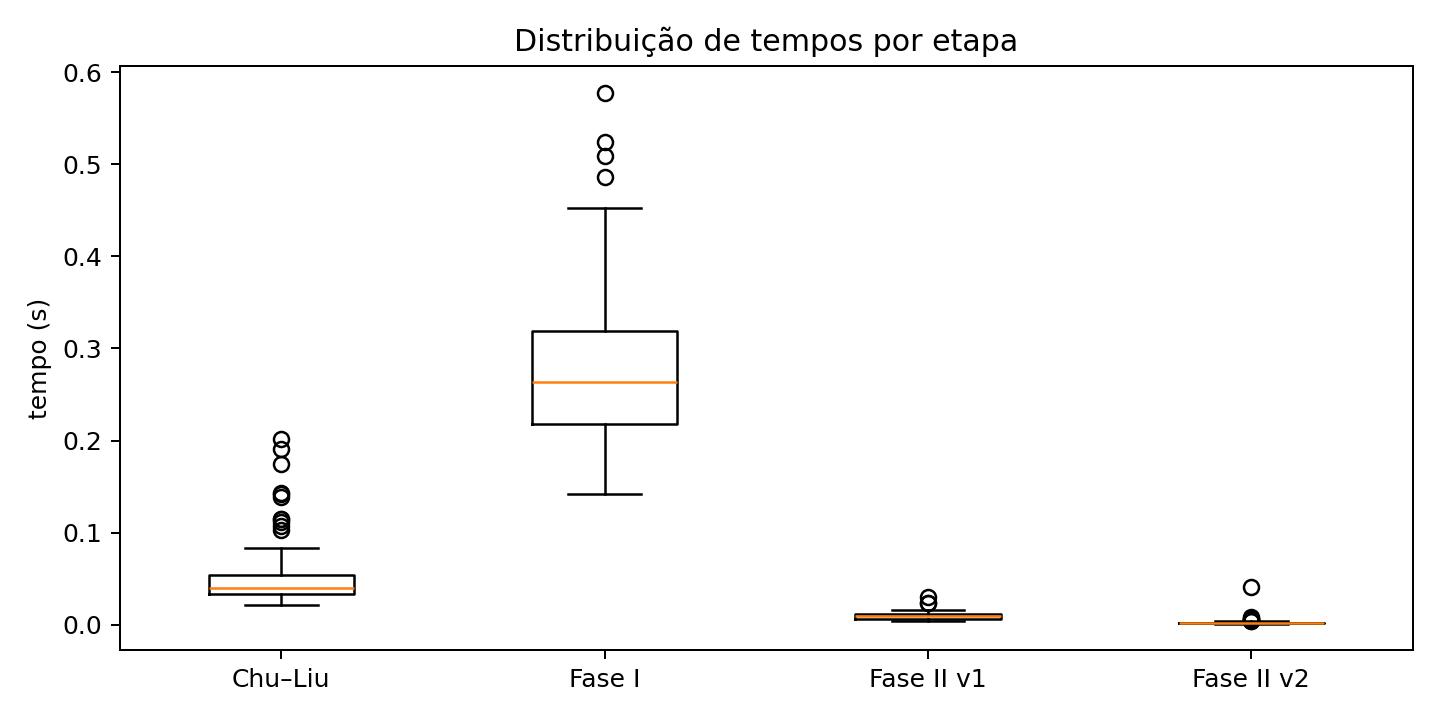
\includegraphics[width=.85\linewidth]{figures/fig_times_boxplot.png}
    \caption{Distribuição de tempos por etapa (boxplot): \emph{Chu--Liu}, Fase~I, Fase~II v1 (direta) e Fase~II v2 (heap).}
    \label{fig:times-boxplot}
\end{figure}

\begin{figure}[H]
    \centering
    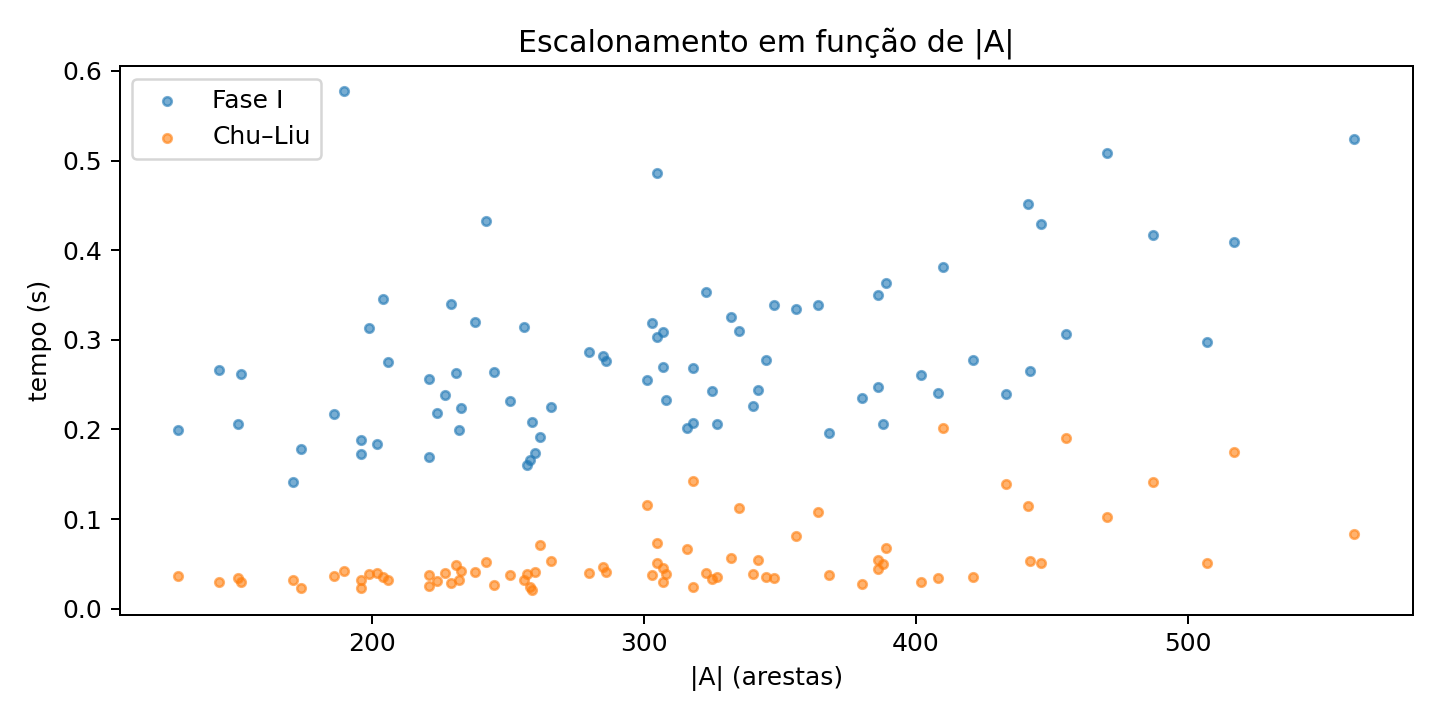
\includegraphics[width=.85\linewidth]{figures/fig_time_vs_edges_scatter.png}
    \caption{Escalonamento temporal em função de \(|A|\): comparação entre \emph{Chu--Liu} e Fase~I.}
    \label{fig:time-vs-edges}
\end{figure}

\begin{figure}[H]
    \centering
    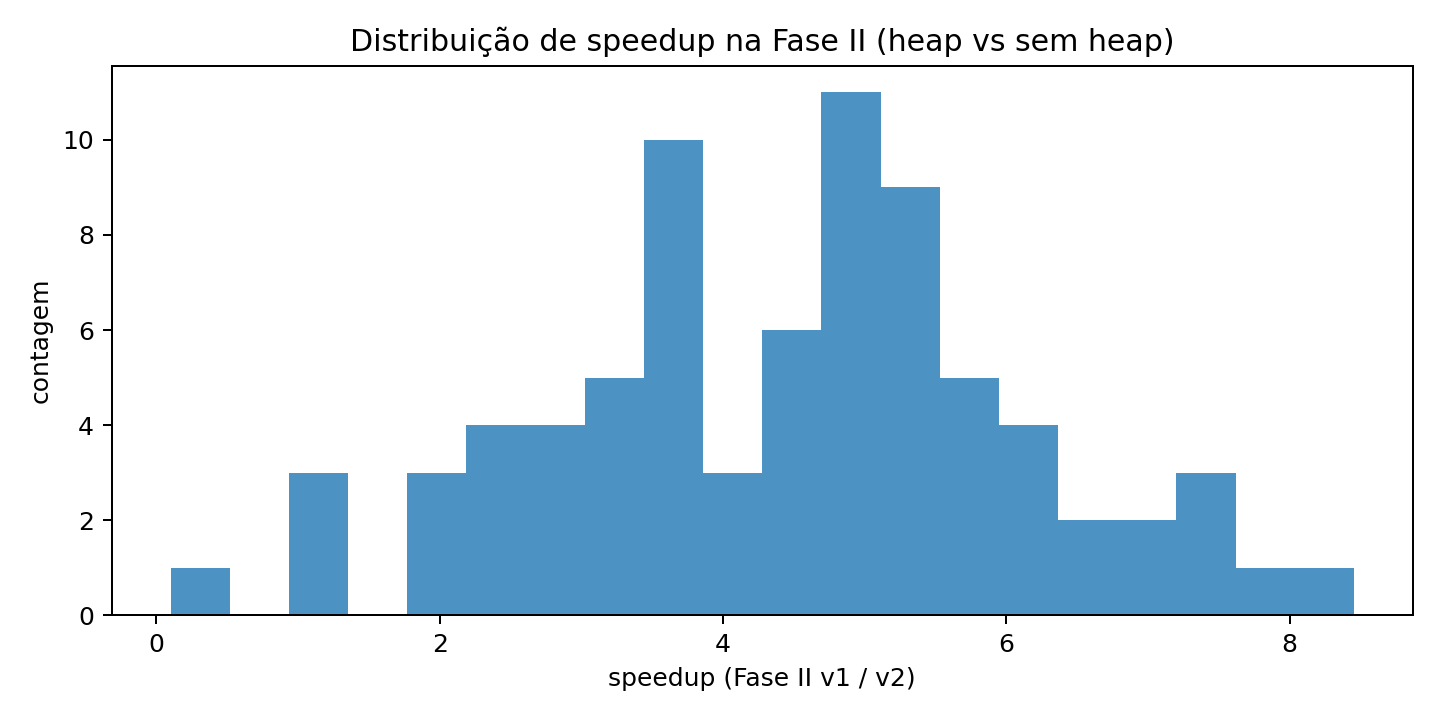
\includegraphics[width=.75\linewidth]{figures/fig_speedup_hist.png}
    \caption{Histograma de speedup na Fase~II (\(\text{v1}/\text{v2}\)): valores maiores que 1 indicam v2 (heap) mais rápida.}
    \label{fig:speedup}
\end{figure}

\begin{figure}[H]
    \centering
    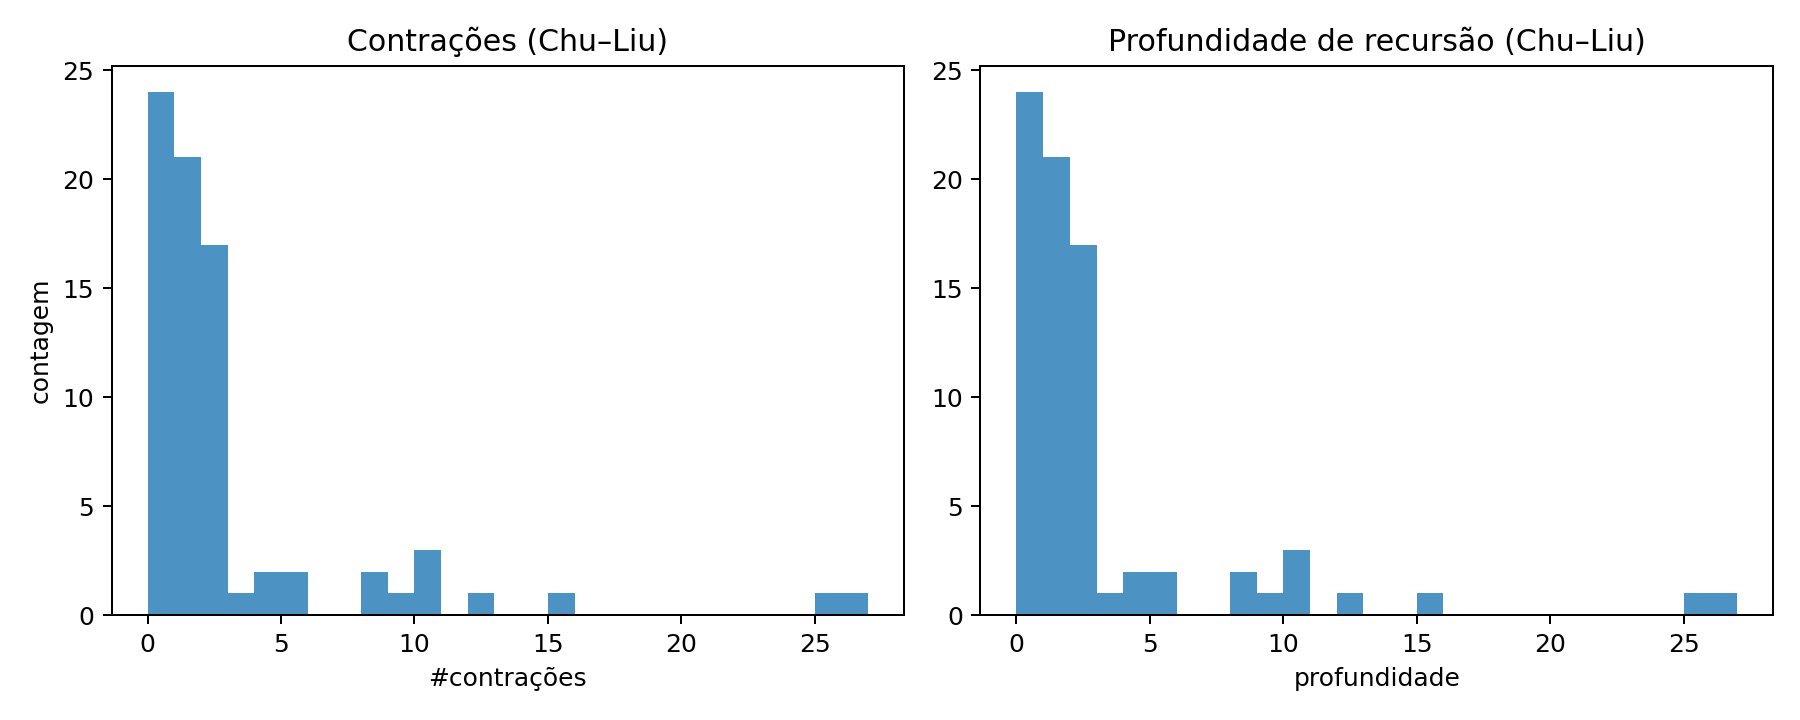
\includegraphics[width=.48\linewidth]{figures/fig_contractions_depth.png}
    \caption{Distribuições do número de contrações e da profundidade de recursão em \emph{Chu--Liu}.}
    \label{fig:contr-depth}
\end{figure}

\begin{figure}[H]
    \centering
    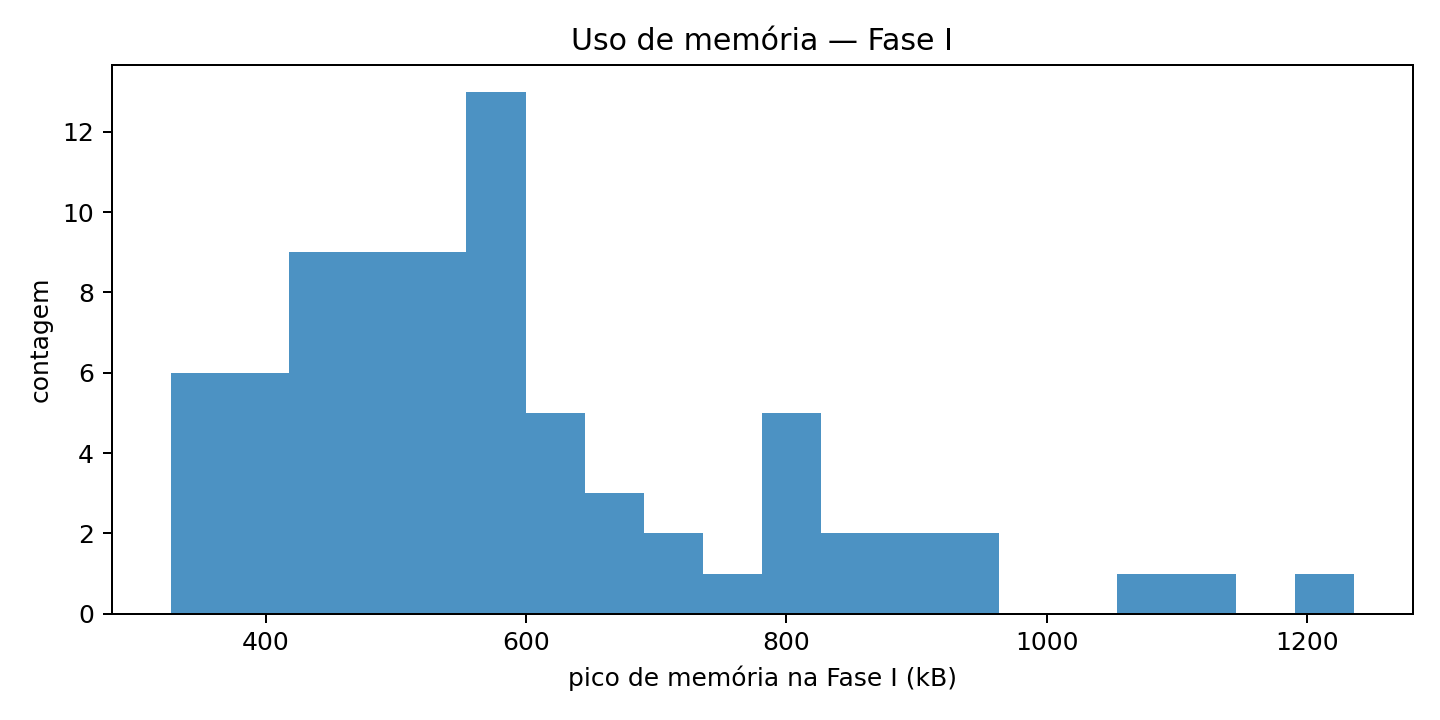
\includegraphics[width=.75\linewidth]{figures/fig_peakmem_hist.png}
    \caption{Pico de memória observado na Fase~I (kB).}
    \label{fig:peakmem}
\end{figure}

\begin{figure}[H]
    \centering
    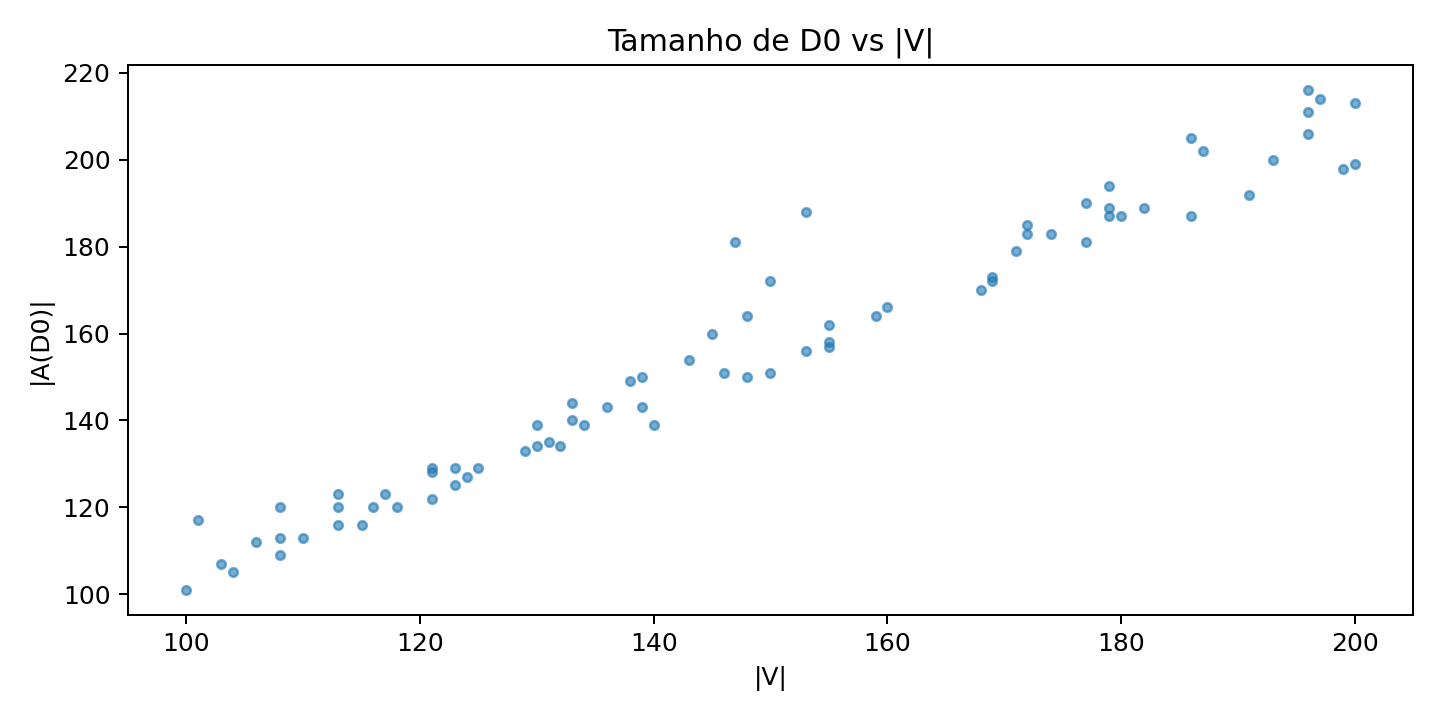
\includegraphics[width=.75\linewidth]{figures/fig_d0_edges_vs_vertices.png}
    \caption{Tamanho de \(D_0\) (número de arestas de custo reduzido zero) em função de \(|V|\).}
    \label{fig:d0-vs-v}
\end{figure}

Em síntese, os resultados empíricos alinham-se às previsões teóricas: custos coincidem e satisfazem complementaridade; o \emph{Chu--Liu} apresenta boa escalabilidade nas faixas testadas; a Fase~I de Frank tende a dominar o tempo; e a variação com heap reduz significativamente o custo da Fase~II, refletindo o uso de extrações \(\log n\). Essas observações reforçam o quadro de \cite{frank2014,schrijver2003comb}: a organização primal--dual de Frank torna explícitas as estruturas (cortes ativos, apertude) que explicam tanto a corretude quanto caminhos de otimização.

\paragraph{}
Em síntese, os testes e as análises oferecem uma base robusta para a compreensão prática e teórica dos algoritmos de arborescência de custo mínimo, explicitando suas forças e nuances. A partir desses achados, avançamos para como transformá-los em aprendizagem efetiva.

\paragraph{}
Para tornar essa experiência concreta, desenvolvemos uma aplicação web interativa que permite acompanhar, passo a passo, o funcionamento de ambos os algoritmos, evidenciando suas semelhanças e diferenças.

\paragraph{}
A aprendizagem visual é especialmente útil: observar os algoritmos em ação ajuda a fixar os conceitos apresentados. A seguir, discutimos aspectos didáticos do ensino de dígrafos em cenários mais complexos e resumimos princípios de interação humano-computador que orientaram o desenho da ferramenta.

\section{A Didática do Abstrato}

\paragraph{}
Thomás de Aquino, em sua obra \emph{De veritate}, argumenta que o conhecimento humano começa com a percepção sensorial do mundo concreto, mas alcança sua plenitude ao transcender o particular e abraçar o universal através da abstração. Esse processo de abstração é fundamental para a matemática e a ciência da computação, onde conceitos complexos são frequentemente representados por meio de símbolos e estruturas que vão além da experiência direta.

\paragraph{}
Grafos e dígrafos são simultaneamente concretos (nós e arestas) e abstratos (propriedades globais como cortes, conectividade, laminaridade). A multiplicidade de noções (caminhos, ciclos, cortes, componentes, condensação) \cite{bondy2008graph,diestel2017graph,west2001introduction}. Essas noções exigem transitar entre níveis de representação (intuitivo, visual, simbólico, formal) \cite{tall1991advanced}, o que pode ser desafiador. A abstração é poderosa, mas também pode ser uma barreira: conceitos como “corte ativo” ou “complementaridade primal–dual” são difíceis de visualizar e internalizar sem apoio didático adequado.

\paragraph{}
Então, como ensinar e aprender conceitos abstratos de forma eficaz? O ensino de matemática no ensino superior, especialmente em áreas como teoria dos grafos parecem sofrer com dificuldades específicas. A seguir, discutimos essas dificuldades e como o uso de ferramentas visuais e interativas pode ajudar a superá-las.

\subsection{Fundamentos cognitivos e didáticos}
\paragraph{}
O ensino de matemática no ensino superior exige transitar entre registros de representação (intuitivo, visual, simbólico, formal) com intencionalidade didática \cite{tall1991advanced}. À luz da teoria da carga cognitiva, é útil distinguir: (i) a \emph{carga intrínseca}, determinada pela complexidade dos esquemas a construir e pelos pré‑requisitos ativados; (ii) a \emph{carga extrínseca}, criada pela forma de apresentação; e (iii) a \emph{carga pertinente} (\emph{germane}), isto é, o esforço dedicado à organização e automatização de esquemas \cite{sweller1988cognitive}. Em cursos avançados, a extrínseca cresce quando definições, símbolos e figuras não são co‑referenciados no tempo e no espaço, dificultando a coordenação entre o que se lê, o que se vê e o que se infere.

\subsubsection{Desafios centrais}
Aprender conteúdos de alta abstração envolve lidar com sobrecarga cognitiva intrínseca e extrínseca \cite{sweller1988cognitive}. Diretrizes de aprendizagem multimídia indicam que combinar representações verbais e visuais pode reduzir carga desnecessária e favorecer integração semântica \cite{mayer2009multimedia,paivio1990}. Em matemática avançada, a transição entre níveis de representação (intuitivo, formal, simbólico) exige mediação cuidadosa \cite{tall1991advanced} e atenção a como exemplos, contraexemplos e invariantes são apresentados.

\paragraph{}
No caso específico de algoritmos com provas baseadas em complementaridade primal--dual, é frequente que estudantes compreendam os passos operacionais sem internalizar a estrutura teórica que garante correção e otimalidade.

\subsubsection{Lidando com grafos e dígrafos}
Na prática, o que mais dificulta o ensino de dígrafos não é definir vértices e arcos, mas articular o que fazemos localmente com as estruturas globais que sustentam as provas de correção e de otimalidade em arborescências de custo mínimo — em particular, nos métodos de Chu–Liu/Edmonds e de Frank —: cortes ativos, componentes fortemente conexas (SCCs) e famílias laminares de conjuntos \cite{bondy2008graph,diestel2017graph,west2001introduction}. Quando essa articulação não aparece, cresce a \emph{carga intrínseca} (múltiplas dependências simultâneas) e também a \emph{carga extrínseca} (o esforço de alinhar texto, fórmulas e figuras). Nesse contexto específico destacamos três desafios didáticos:
\begin{itemize}\setlength{\itemsep}{2pt}
    \item \textbf{Articular o local com o global:} escolher a melhor aresta de entrada para cada vértice não garante coerência global; isso pode criar ciclos. Ver o grafo \emph{condensado} em SCCs (cada ciclo vira um ``bloco'') torna esse efeito visível e manipulável (Fig.~\ref{fig:didatica-condensado}). \emph{Dificuldade típica:} estudantes tendem a projetar a heurística local para o todo e se surpreendem com ciclos “inesperados” — uma fonte comum de sobrecarga por conflito entre intuições locais e restrições globais.
    \item \textbf{Acompanhar efeitos de contração/expansão:} contrair um ciclo (substituí\-lo por um supervértice) e depois reexpandir impacta os custos reduzidos \(c'\) e os cortes que ficam ``ativos''. A laminaridade — cortes aninhados, sem interseções conflitantes — fornece uma geometria simples para seguir essas mudanças (Fig.~\ref{fig:didatica-laminar}). \emph{Dificuldade típica:} perder o fio entre representações (grafo original, condensado, reexpansão) aumenta a carga extrínseca; sinalizar o que mudou em cada etapa reduz esse atrito.
    \item \textbf{Mapear o ``fazer do algoritmo'' para a linguagem primal–dual:} ações como elevar potenciais, escolher entradas e contrair ciclos correspondem a garantias teóricas. Em particular, \emph{apertude} (custo reduzido zero) e \emph{complementaridade} (exatamente uma aresta entra em cada conjunto ativo) certificam a otimalidade. Relacionar essas ideias às métricas que coletamos (tempos, número de contrações, pico de memória) ajuda a ligar prática e teoria, via custos reduzidos e reexpansão (Figs.~\ref{fig:didatica-reduced-cost} e \ref{fig:didatica-reexpansion}). \emph{Dificuldade típica:} executar os passos sem ver como eles tornam certas restrições “justas” dificulta a internalização do porquê; explicitar os vínculos entre ação e certificação reduz a distância entre o operacional e o conceitual.
\end{itemize}

\paragraph{}
No exemplo da figura abaixo, a condensação do dígrafo \(D\) em \(D_0\) torna visível a relação entre escolhas locais (entradas por vértice) e estrutura global (ciclos, cortes). Cada SCC (bloco) pode ser tratado como uma unidade, facilitando a compreensão de como ciclos surgem e são resolvidos. Apesar de não ser suficiente para ilustrar situações mais complexas, essa visualização ajuda criar intuição sobre a atualização de custos reduzidos e a dinâmica de contração/expansão.

\begin{figure}[H]
    \centering
    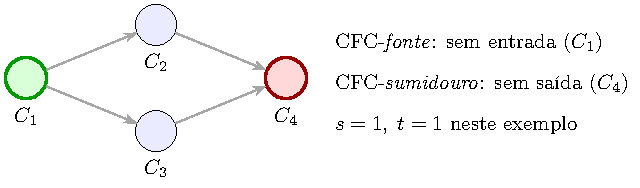
\includegraphics[width=.72\linewidth]{figures/fig_condensado_st.pdf}
    \caption{Condensação de $D_0$ e fontes do DAG: ver o grafo “como” blocos (SCCs) ajuda a articular o local (entradas por vértice) com o global (cortes e contrações).}
    \label{fig:didatica-condensado}
\end{figure}

\subsection{Visualização e interação: princípios em uso}
Há evidências de que diagramas e animações, quando bem projetados, podem acelerar a compreensão de relações topológicas e causais \cite{larkin1987diagram,ware2012information}.

\paragraph{}
A teoria da carga cognitiva sugere que combinar representações verbais e visuais pode reduzir carga extrínseca e favorecer integração semântica \cite{mayer2009multimedia,paivio1990}. Diretrizes de aprendizagem multimídia recomendam evitar excesso de elementos visuais que não contribuam para o entendimento (reduzindo carga extrínseca) e alinhar texto e imagens no tempo e no espaço (reduzindo esforço de coordenação) \cite{mayer2009multimedia}.

\paragraph{}
No campo específico de matemática avançada, Tall enfatiza a coordenação entre registros — intuitivo, visual, simbólico e formal — como motor da passagem do pensamento predominantemente procedimental para o conceitual \cite{tall1991advanced}. Diagramas não são meros adornos: estruturam inferências espaciais e relacionais de modo mais eficiente que sentenças lineares \cite{larkin1987diagram}.


\paragraph{}
Na educação em ciência da computação, visualizações de algoritmos têm efeito positivo sobretudo quando promovem \emph{engajamento ativo} (prever, manipular, explicar) e não apenas consumo passivo \cite{hundhausen2002meta,naps2003engagement}.

\subsection{Disseminação de conteúdos avançados: o ecossistema de ferramentas}

\paragraph{}
Materiais que conectam teoria, evidências empíricas e interatividade têm maior potencial de transferência e retenção. 

\paragraph{}
Tendo em vista esses fundamentos, ferramentas digitais podem ajudar a reduzir carga extrínseca e a integrar registros (visual, simbólico, formal) quando a interação é desenhada para promover \emph{engajamento ativo} \cite{mayer2009multimedia,sweller1988cognitive,hundhausen2002meta,naps2003engagement}. A seguir, apresentamos categorias de ferramentas úteis no ensino de grafos, indicando finalidades, forças e limitações, e posicionamos a nossa aplicação nesse ecossistema.

\subsubsection{Ferramentas didáticas no ensino de teoria dos grafos}
\paragraph{}
Várias ferramentas digitais podem apoiar o ensino de grafos e dígrafos, cada uma com forças e limitações específicas. A seguir, discutimos quatro categorias principais: (i) diagramas programáveis e tipografia matemática, (ii) exploração e edição de grafos, (iii) visualização de algoritmos, e (iv) ambientes programáveis e reprodutibilidade.

\paragraph{Diagramas e matemática}
\paragraph{}
Algumas ferramentas permitem criar diagramas de grafos com semântica visual consistente, integrando-os a textos matemáticos. Essas ferramentas são úteis para ilustrar conceitos, definições e provas em materiais didáticos.

\paragraph{}
Ambientes como Graphviz/dot e TikZ/PGF permitem especificar grafos declarativamente e gerar figuras reprodutíveis com layouts consistentes \cite{graphviz,tantau2015tikz}. Benefícios didáticos: (i) semântica visual estável (mesmo conceito, mesma forma), (ii) autoria próxima ao símbolo e ao texto (co-referência), (iii) manutenção e versionamento fáceis. Limitações: a interação costuma ser offline (figuras estáticas) e a curva de aprendizado de sintaxe pode ser um obstáculo inicial. Em contextos de prova e definição, esses recursos ancoram a narrativa formal com diagramas que obedecem às diretrizes de \cite{larkin1987diagram,ware2012information}.

\paragraph{}
Contudo, diagramas estáticos não capturam a dinâmica de algoritmos que envolvem mudanças estruturais (elevação de potenciais, contração/expansão, seleção de arestas). Para isso, são necessárias ferramentas interativas que permitam explorar essas transformações em tempo real.

\paragraph{Exploração e edição de grafos}
\paragraph{}
Ferramentas de exploração e edição de grafos permitem que os usuários interajam com representações gráficas de dados, facilitando a manipulação e a análise de estruturas complexas. Essas ferramentas são essenciais para atividades que exigem uma compreensão profunda das relações entre os elementos de um grafo.


\paragraph{}
Dentre elas destacam-se Gephi, yEd e Cytoscape oferecem layouts automáticos, filtros e medidas de rede \cite{bastian2009gephi,yed,shannon2003cytoscape}. São adequadas para: (i) reconhecer padrões estruturais (componentes, comunidades), (ii) discutir implicações de layouts para percepção de estruturas, (iii) atividades de descoberta assistida ("overview \textrightarrow{} filter \textrightarrow{} details") \cite{shneiderman1996eyes}. Limitações: (i) foco em análise exploratória de dados, não em algoritmos específicos; (ii) carga extrínseca ao alternar entre interface gráfica e conceitos teóricos; (iii) falta de controle fino sobre estados intermediários de algoritmos.

\paragraph{Visualização de algoritmos}
\paragraph{}
Existem diversas ferramentas dedicadas à visualização de algoritmos, que ilustram passo a passo como um algoritmo opera sobre uma estrutura de dados. 

\paragraph{}
Repositórios e portais como VisuAlgo e iniciativas similares apresentam animações de algoritmos clássicos com controle do ritmo e de estados \cite{visualgo,hundhausen2002meta,naps2003engagement}. Evidências sugerem ganhos quando o estudante prevê, manipula e explica o que vê, ao invés de consumir animações passivamente. Pontos de atenção: (i) alinhar a animação às noções teóricas subjacentes (invariantes, certificados), (ii) explicitar mapeamentos entre "o que acontece" e "o que se garante" (p.ex., custo reduzido zero \(c'=0\), complementaridade), (iii) evitar excesso de elementos visuais que aumentem carga extrínseca \cite{mayer2009multimedia}.

\paragraph{Ambientes programáveis e reprodutibilidade}
\paragraph{}
Ferramentas como Jupyter Notebooks e bibliotecas como NetworkX permitem combinar código, texto e visualizações em um único documento interativo \cite{kluyver2016jupyter,hagberg2008networkx}. Essas ferramentas são valiosas para criar exemplos reprodutíveis e explorar algoritmos de forma prática.

\paragraph{}
Contudo, requerem familiaridade com programação e podem introduzir carga extrínseca se o foco se desviar para detalhes de implementação. A curadoria do conteúdo é essencial para manter o foco didático e evitar dispersão.

\paragraph{}
Tendo em vista essas categorias, desenvolvemos uma aplicação web interativa que combina elementos de visualização de algoritmos e ambientes programáveis, com foco específico nos algoritmos de arborescência de custo mínimo. A seguir, apresentamos princípios envolvendo a teoria de interação humano-computador que orientaram o desenho da ferramenta, e em seguida descrevemos a aplicação com seus respectivos detalhes de implementação e como ela se posiciona nesse ecossistema.


\section{A interação humano--computacional em ação: uma aplicação web interativa}

\paragraph{}
A aplicação web interativa foi desenvolvida para ilustrar os algoritmos de Chu–Liu/Edmonds e Frank, permitindo aos usuários acompanhar passo a passo o funcionamento de ambos os métodos. A ferramenta foi projetada com base em princípios de interação humano-computador, visando maximizar a compreensão e o engajamento dos usuários.

\subsection{Princípios de interação humano-computador}

\paragraph{}
A interação humano-computador (IHC) estuda como projetar sistemas computacionais que sejam eficientes, eficazes e agradáveis para os usuários. 

\paragraph{}
Sintetizando heurísticas de usabilidade e descoberta \cite{nielsen1994heuristics,shneiderman2016designing} e quadros de interação e aprendizagem \cite{rogers2011interaction,mayer2009multimedia,sweller1988cognitive,naps2003engagement}, destacamos oito princípios orientadores: (i) usabilidade, (ii) eficiência cognitiva, (iii) feedback imediato, (iv) engajamento ativo, (v) visão geral com detalhe sob demanda (mantra \emph{overview→filter→details} de \cite{shneiderman1996eyes}), (vi) consistência semântica, (vii) múltiplos registros de representação e (viii) prevenção/recuperação de erros. A seguir descrevemos cada um e sua materialização na ferramenta.


\paragraph{Usabilidade}
\paragraph{}
Usabilidade refere-se à facilidade com que os usuários podem aprender a usar um sistema, realizar tarefas e alcançar seus objetivos. Na nossa aplicação, priorizamos uma interface limpa e intuitiva, com controles claros para navegar pelos passos dos algoritmos, selecionar arestas, visualizar cortes ativos e entender a evolução dos custos reduzidos.

\paragraph{Eficiência cognitiva}
\paragraph{}
Eficiência cognitiva envolve minimizar a carga cognitiva dos usuários, facilitando a compreensão e o processamento de informações. Implementamos visualizações que destacam mudanças importantes (como contrações e expansões) e fornecem explicações textuais concisas para cada passo, ajudando os usuários a conectar ações com conceitos teóricos.

\paragraph{Feedback Imediato}
\paragraph{}
Feedback imediato é crucial para manter os usuários informados sobre o estado do sistema e as consequências de suas ações. Nossa ferramenta oferece feedback visual e textual em tempo real, mostrando como cada ação afeta o grafo e os custos associados, reforçando a compreensão causal.

\paragraph{Engajamento ativo}
\paragraph{}
Engajamento ativo refere-se à participação dos usuários no processo de aprendizagem, incentivando-os a explorar, experimentar e interagir com o sistema. Nossa aplicação promove o engajamento ativo ao permitir que os usuários manipulem o grafo, testem diferentes abordagens e visualizem os resultados de suas ações em tempo real.


\paragraph{Visão geral com detalhe sob demanda}
\paragraph{}
A visão geral com detalhe sob demanda permite que os usuários obtenham uma compreensão ampla do sistema, enquanto ainda têm acesso a informações detalhadas quando necessário. Implementamos essa abordagem ao fornecer uma visualização geral do grafo, com a opção de expandir informações sobre arestas e nós específicos conforme o interesse do usuário.

\paragraph{Consistência semântica}
\paragraph{}
A consistência semântica garante que os elementos da interface e suas interações sejam compreensíveis e previsíveis. Nossa ferramenta mantém a consistência semântica ao usar terminologia e representações visuais padronizadas em toda a aplicação, facilitando a compreensão dos usuários.

\paragraph{Múltiplos registros de representação}
\paragraph{}
Múltiplos registros de representação referem-se à capacidade de apresentar informações de diferentes maneiras, atendendo às preferências e estilos de aprendizagem dos usuários. Nossa aplicação oferece várias representações do grafo (visual, textual, interativa), permitindo que os usuários escolham a forma que melhor se adapta às suas necessidades.

\paragraph{Prevenção de erros}
\paragraph{}
A prevenção de erros envolve projetar o sistema de forma a minimizar a probabilidade de erros dos usuários. Implementamos medidas de prevenção de erros, como validação de entrada e feedback em tempo real, para ajudar os usuários a evitar ações indesejadas e compreender melhor as consequências de suas escolhas.

\paragraph{}
Esses princípios de interação humano-computador foram fundamentais para o desenvolvimento da nossa aplicação web interativa, garantindo que ela seja não apenas funcional, mas também acessível e eficaz como ferramenta de aprendizagem. A seguir, detalhamos a implementação técnica da aplicação e como ela se posiciona no ecossistema de ferramentas didáticas para o ensino de grafos.

\begin{table}[H]
    \centering
    \renewcommand{\arraystretch}{1.18}
    \setlength{\tabcolsep}{6pt}
    \footnotesize
    % Ajuste de larguras: 1a coluna ampliada para evitar overlap; leve redução na 3a.
    \begin{tabular}{p{2.9cm} p{4.0cm} p{7.0cm}}
        \hline
        	\textbf{Princípio} & \textbf{Exemplo Geral} & \textbf{Materialização na Aplicação} \\
        \hline
    Usabilidade & Botões claros para avançar/voltar etapas & Barra de controles com rótulos diretos (Adicionar Aresta, Executar, Reset); agrupamento visual consistente via Tailwind; nenhum menu profundo aninhado. \\
    Eficiência\newline cognitiva & Reduzir elementos irrelevantes no estado atual & Layout estável entre passos; apenas arestas relevantes destacadas; eliminação de ornamentação visual; custos e rótulos legíveis sem rotação. \\
    Feedback\newline imediato & Mostrar efeito de uma ação logo após o clique & Cada ação dispara: (i) atualização do desenho do grafo, (ii) entrada no log textual explicando a mudança (ex.: contração, seleção de aresta). \\
    Engajamento\newline ativo & Usuário prediz antes de revelar próximo passo & Controles passo a passo permitem explorar sequencialmente; usuário insere/edita pesos e escolhe raiz antes de rodar o algoritmo. \\
    Overview→\newline Details & Visão global com acesso a informação pontual & Visão completa do grafo em todos os passos + possibilidade de inspecionar pesos e arestas específicas no log sequencial; estados anteriores preservados para comparação mental. \\
    Consistência\newline semântica & Mesmo conceito, mesma cor/forma & Raiz destacada de forma fixa; arestas selecionadas mantêm estilo; semântica cromática não muda entre passos (evita remapeamento mental). \\
    Múltiplos\newline registros & Texto + grafo + (futuro) estrutura derivada & Combinação de: descrição textual no log, representação visual do grafo, parâmetros simbólicos (pesos); prepara expansão futura para mostrar custos reduzidos. \\
    Prevenção /\newline recuperação\newline de erros & Impedir entrada inválida / ação reversível & Validação de pesos (numéricos); bloqueio de execução sem raiz definida; botão Reset para recompor estado limpo sem recarregar página. \\
        \hline
    \end{tabular}
    \caption{Síntese dos princípios de interação humano-computador aplicados e sua realização concreta na ferramenta interativa.}
    \label{tab:principios-ihc}
\end{table}

\subsection{Descrição da aplicação}
\paragraph{}
A aplicação web interativa foi desenvolvida para ilustrar os algoritmos de Chu–Liu/Edmonds e Frank, permitindo aos usuários acompanhar passo a passo o funcionamento de ambos os métodos. A ferramenta foi projetada com base em princípios de interação humano-computador, visando maximizar a compreensão e o engajamento dos usuários.


\subsubsection{Visão geral das páginas}
A aplicação web é composta por páginas HTML autônomas carregadas no navegador, cada uma focada em um aspecto: (i) \texttt{home.html} (apresentação / resumo), (ii) \texttt{chuliu.html} (execução passo a passo do algoritmo de Chu--Liu/Edmonds), (iii) \texttt{andrasfrank.html} (estrutura para futura visualização da abordagem primal--dual), (iv) \texttt{draw\_graph.html} (editor livre de grafos), além do componente compartilhado de navegação lateral \texttt{sidebar.html}. Cada página injeta o \texttt{sidebar} dinamicamente e carrega scripts específicos.

\paragraph{Bibliotecas e dependências}

\paragraph{}
O desenvolvimento utilizou tecnologias web modernas, incluindo HTML5, Tailwind CSS para estilos responsivos, e PyScript para execução de código Python diretamente no navegador. A biblioteca NetworkX foi empregada para manipulação de grafos, enquanto Matplotlib gerou visualizações estáticas dos estados intermediários. O código foi estruturado para modularidade e clareza, facilitando futuras extensões. Detalhamos abaixo esses aspectos:

\begin{itemize}\setlength{\itemsep}{2pt}
    \item \textbf{Frontend:} HTML5 + Tailwind CSS para composição responsiva e estilos utilitários consistentes.
    \item \textbf{Execução Python no cliente:} PyScript (carregado via CDN) provê execução de módulos Python (ex.: \texttt{networkx}, \texttt{matplotlib}) sem instalação local, reduzindo barreira de entrada didática.
    \item \textbf{Bibliotecas centrais:} NetworkX para manipulação de grafos dirigidos; \texttt{matplotlib} para renderização de snapshots; (em páginas avançadas) Cytoscape.js previsto para interação rica (estrutura já importada em \texttt{chuliu.html} / \texttt{andrasfrank.html}).
    \item \textbf{Empacotamento de estado:} Serialização JSON (formato \texttt{node\_link}) para exportação e reuso analítico.
    \item \textbf{Isolamento:} Cada página carrega apenas os elementos necessários, evitando \emph{payload} excessivo e minimizando latência de interface (princípio de eficiência cognitiva).
\end{itemize}

\paragraph{Componentes funcionais principais}
\paragraph{}
A aplicação centraliza-se nas páginas \texttt{chuliu.html} e \texttt{andrasfrank.html}, que permitem executar os algoritmos de Chu--Liu/Edmonds e Frank, respectivamente. A seguir, detalhamos os componentes funcionais principais da interface:

\begin{enumerate}\setlength{\itemsep}{2pt}
    \item \textbf{Editor de Grafo:} Inputs para origem, destino e peso + botões de inserção e limpeza (\texttt{add-edge}, \texttt{reset-graph}).
    \item \textbf{Carregamento de exemplo:} Botão \texttt{load-test-graph} injeta um grafo de teste estruturado para reduzir \emph{time-to-first-insight}.
    \item \textbf{Configuração de raiz:} Campo para definir / confirmar o vértice raiz (\texttt{root-node}).
    \item \textbf{Execução algorítmica:} Botão \texttt{run-algorithm} dispara o pipeline de filtragem e cálculo da arborescência mínima.
    \item \textbf{Visualização de estados:} Área cumulativa (\texttt{graph-area}) onde cada renderização mantém a coerência posicional (layout determinístico) para comparação mental entre passos.
    \item \textbf{Log textual:} Caixa de texto incremental (\texttt{log-output}) correlaciona ações a transformações estruturais (dual coding: texto + imagem).
    \item \textbf{Exportação:} Ação de exportar grafo em JSON para análise posterior ou reimportação.
    \item \textbf{Incorporação de PDF:} \texttt{tese.html} exibe o \texttt{main.pdf} lado a lado à aplicação, incentivando leitura entrelaçada teoria-execução.
\end{enumerate}

\paragraph{Fluxo de interação}
\paragraph{}
O fluxo de interação foi projetado para ser linear e intuitivo, guiando o usuário desde a criação do grafo até a visualização dos resultados do algoritmo. A seguir, descrevemos o fluxo típico:

\begin{enumerate}\setlength{\itemsep}{2pt}
    \item Usuário monta ou carrega um grafo de teste.
    \item Define (ou confirma) o vértice raiz \(r_0\).
    \item Executa o algoritmo (Chu--Liu/Edmonds): são aplicadas normalizações e seleção de arestas (implementação apresentada em seções anteriores / listagens).
    \item Observa estados sequenciais: cada snapshot reforça invariantes (arestas escolhidas, pesos, estrutura alcançada).
    \item (Opcional) Exporta o grafo resultante para replicação em notebooks ou comparação com a abordagem dual futura.
\end{enumerate}

\paragraph{Estado e dados persistentes}
\paragraph{}    
O estado principal é mantido em memória (objeto \texttt{networkx.DiGraph}). O log textual funciona como uma \emph{trilha de auditoria didática}. Cada ação do usuário (adição de aresta, definição de raiz, execução de passo) atualiza o grafo e o log, permitindo rastrear a evolução do estado. A exportação em JSON facilita a reimportação e análise posterior.

\paragraph{Limitações atuais}
\paragraph{}
Atualmente, a aplicação apresenta algumas limitações que podem impactar a experiência do usuário e a eficácia da visualização:

\begin{itemize}\setlength{\itemsep}{2pt}
    \item Ausência de visualização explícita de contração de ciclos (marcação diferenciada por cores/aglomerados ainda não implementada).
    \item Não há comparação lado a lado (split view) entre algoritmos (Chu--Liu vs. Frank) ainda.
    \item Layout planar simples pode falhar em instâncias mais densas (sobreposição de rótulos) — futura substituição por \texttt{spring} ou \texttt{dagre}-like adaptativo.
    \item Falta camada de destaque cromático para custos reduzidos e arcos “apertados” \((c' = 0)\).
    \item Exportação limita-se ao grafo final; não há pacote de estados intermediários (\emph{replay}).
\end{itemize}

\paragraph{Melhorias futuras}
\paragraph{}
Desse modo, entendemos que a aplicação, embora funcional, pode ser aprimorada com recursos adicionais para enriquecer a experiência didática. Algumas melhorias incluem:

\begin{itemize}\setlength{\itemsep}{2pt}
    \item Visualização animada da contração/reexpansão de ciclos com agrupamento colapsável.
    \item Camada de coloração para arestas com custo reduzido zero e cortes ativos.
    \item Geração automática de relatório (log + estados selecionados) em PDF/ZIP.
    \item Módulo paralelo para a abordagem primal--dual de Frank (empacotamento de cortes e duas fases).
    \item Modo “comparativo” exibindo diferenças de passos e métricas agregadas.
    \item Instrumentação de métricas (tempo por passo, número de contrações, distribuição de pesos normalizados).
\end{itemize}

\paragraph{}
De modo geral, a aplicação serve como um protótipo funcional que demonstra o potencial de ferramentas interativas para o ensino de algoritmos complexos em teoria dos grafos. Com melhorias contínuas, pode se tornar uma plataforma robusta para aprendizagem ativa e visualização didática. Na seção seguinte, detalhamos aspectos técnicos da implementação.

\subsection{Detalhes de Implementação}
\paragraph{}
A aplicação foi implementada utilizando tecnologias web modernas, com foco em simplicidade, modularidade e reprodutibilidade. A seguir, detalhamos os principais aspectos técnicos da implementação.

\paragraph{Estrutura de arquivos}
\paragraph{}
A estrutura de arquivos da aplicação é organizada da seguinte forma:
\begin{itemize}\setlength{\itemsep}{2pt}
    \item \texttt{main.py}: Script Python principal contendo funções de manipulação de grafos e lógica algorítmica.
    \item \texttt{index.html}: Página inicial com resumo e links para outras seções.
    \item \texttt{chuliu.html}: Página dedicada à execução do algoritmo de Chu--Liu/Edmonds.
    \item \texttt{andrasfrank.html}: Página para futura implementação do algoritmo de Frank.
    \item \texttt{draw\_graph.html}: Editor livre de grafos.
    \item \texttt{sidebar.html}: Componente de navegação lateral compartilhado.
    \item \texttt{styles.css}: Arquivo de estilos customizados (além do Tailwind).
    \item \texttt{scripts/}: Diretório contendo scripts Python e JavaScript.
    \item \texttt{assets/}: Diretório para imagens, ícones e outros recursos estáticos.
\end{itemize}

\subsubsection{Códigos principais}
\paragraph{}
A seguir, apresentamos os códigos desenvolvidos para os algoritmos implementados realizarem a interação com os usuários.

\paragraph{\texttt{Main.py}:} o arquivo \texttt{main.py} contém funções para manipulação de grafos, execução dos algoritmos e geração de visualizações.

\paragraph{}
As funções principais incluem:
\begin{itemize}\setlength{\itemsep}{2pt}
    \item \texttt{draw\_graph(G, title, append)}: Renderiza o grafo \(G\) com título e opção de anexar ou substituir a visualização.
    \item \texttt{add\_edge()}: Adiciona uma aresta ao grafo com base nos inputs do usuário.
    \item \texttt{reset\_graph()}: Limpa o grafo atual e o log.
    \item \texttt{export\_graph()}: Exporta o grafo atual em formato JSON.
    \item \texttt{load\_test\_graph()}: Carrega um grafo de teste predefinido.
    \item \texttt{run\_algorithm()}: Executa o algoritmo de Chu--Liu/Edmonds, aplicando filtragem e visualizando cada passo.
\end{itemize}

A seguir, apresentamos essas funções conforme implementadas no arquivo \texttt{main.py}.

\begin{pybox}[label={lst:draw_graph}]{Main.py: manipulação e visualização de grafos}
import networkx as nx
from networkx.readwrite import json_graph
import matplotlib.pyplot as plt
from js import Blob, URL, document, alert
from pyscript import when, display
import json

from chuliu import find_optimum_arborescence_chuliu, remove_edges_to_r0

def log_in_box(msg: str):
    log_box = document.getElementById("log-output")
    log_box.value += msg + "\n"
    log_box.scrollTop = log_box.scrollHeight

def draw_graph(G: nx.DiGraph, title="Digrafo", append=True):
    plt.clf()  # Limpa a figura atual
    pos = nx.planar_layout(G)  # Layout para posicionamento dos nós
    plt.figure(figsize=(6, 4))  # Tamanho da figura
    # Desenha os nós e arestas
    nx.draw(
        G,
        pos,
        with_labels=True,
        node_color="lightblue",
        edge_color="gray",
        node_size=2000,
        font_size=12,
    )
    weights = nx.get_edge_attributes(G, "w")
    nx.draw_networkx_edge_labels(
        G, pos, edge_labels=weights, font_color="red", font_size=12
    )
    plt.title(title)
    display(title, target="graph-area", append=append)
    display(plt, target="graph-area", append=append)
    plt.close()  # Fecha a figura para liberar memória

G = nx.DiGraph()

@when("click", "#add-edge")
def add_edge():
    global G
    source = document.getElementById("source").value
    target = document.getElementById("target").value
    weight = document.getElementById("weight").value
    if source and target and weight:
        G.add_edge(source, target, w=float(weight))
        log_in_box(f"Aresta adicionada: {source} → {target} (peso={weight})")
        draw_graph(G, "Grafo com Arestas", append=False)

@when("click", "#reset-graph")
def reset_graph():
    global G
    G.clear()
    document.getElementById("log-output").value = ""
    draw_graph(G, "Grafo Resetado", append=False)
    log_in_box("Grafo resetado.")

@when("click", "#export-graph")
def export_graph(event):
    log_in_box("Exportando grafo...")
    global G
    if G.number_of_nodes() == 0:
        log_in_box("[ERRO] O grafo está vazio.")
        return

    # Converte o grafo para JSON
    data = json_graph.node_link_data(G, edges="links")
    json_data = json.dumps(data, indent=4)

    # Cria um link de download no navegador
    blob = Blob.new([json_data], {"type": "application/json"})
    url = URL.createObjectURL(blob)

    # Configura e dispara o download
    link = document.createElement("a")
    link.href = url
    link.download = "graph_teste.json"
    link.click()
    URL.revokeObjectURL(url)

    log_in_box("Download do grafo iniciado.")

@when("click", "#load-test-graph")
def load_test_graph(event):
    global G
    G.clear()
    G.add_edge("r0", "B", w=10)
    G.add_edge("r0", "A", w=2)
    G.add_edge("r0", "C", w=10)
    G.add_edge("B", "A", w=1)
    G.add_edge("A", "C", w=4)
    G.add_edge("C", "D", w=2)
    G.add_edge("D", "B", w=2)
    G.add_edge("B", "E", w=8)
    G.add_edge("C", "E", w=4)

    log_in_box("Grafo de teste carregado.")
    draw_graph(G, "Grafo de Teste (DG)", append=False)

@when("click", "#show-ready-arborescence")
def show_ready_arborescence(event):
    T = nx.DiGraph()
    T.add_edge("r0", "A", w=2)
    T.add_edge("A", "C", w=4)
    T.add_edge("C", "D", w=2)
    T.add_edge("D", "B", w=2)
    T.add_edge("C", "E", w=4)
    draw_graph(T, "Arborescência Pré-definida")
    log_in_box("Arborescência pronta exibida.")


@when("click", "#run-algorithm")
def run_algorithm(event):
    global G
    r0 = document.getElementById("root-node").value or "r0"
    if r0 not in G:
        alert(f"[ERRO] O nó raiz '{r0}' deve existir no grafo.")
        return

    log_in_box("Executando algoritmo de Chu-Liu...")
    print(remove_edges_to_r0)
    G_filtered = remove_edges_to_r0(G, r0)
    T = find_optimum_arborescence_chuliu(
        G_filtered, r0, draw_fn=draw_graph, log=log_in_box
    )
    draw_graph(T, "Arborescência Ótima")
    log_in_box("Execução concluída com sucesso.")
\end{pybox}

\paragraph{\texttt{Index.html}:} o arquivo \texttt{index.html} define a estrutura principal da página HTML, incluindo a integração com PyScript e Tailwind CSS para estilos responsivos. A seguir, apresentamos o código completo dessa página.     

\begin{htmlbox}[label={lst:index_html}]{Estrutura principal da página HTML com PyScript}
<!DOCTYPE html>
<html>
  <head>
    <meta charset="utf-8" />
    <meta name="viewport" content="width=device-width,initial-scale=1" />
    <title>Chu-Liu/Edmonds Visualizer</title>
    <script src="https://cdn.tailwindcss.com"></script>
    <link
      rel="stylesheet"
      href="https://pyscript.net/releases/2025.3.1/core.css"
    />
    <script
      type="module"
      src="https://pyscript.net/releases/2025.3.1/core.js"
    ></script>
  </head>
  <body class="bg-gray-100">
    <header class="bg-[#5b8f79] text-white text-center p-6">
      <h1 class="text-3xl font-bold">Chu-Liu/Edmonds Visualizer</h1>
      <p class="text-lg mt-2">
        Visualização passo a passo de arborescências em grafos direcionados
      </p>
    </header>

    <main class="flex flex-col items-center gap-8 py-8 px-8">
      <section class="text-center w-full max-w-4xl">
        <h2 class="text-2xl font-semibold text-[#5b8f79] mb-4">
          Definir Di-grafo
        </h2>
        <div class="flex flex-wrap justify-center gap-4 items-center mb-4">
          <input
            type="text"
            id="source"
            placeholder="Origem"
            class="p-3 border rounded border-gray-300 w-40"
          />
          <input
            type="text"
            id="target"
            placeholder="Destino"
            class="p-3 border rounded border-gray-300 w-40"
          />
          <input
            type="number"
            id="weight"
            placeholder="Peso"
            min="0"
            class="p-3 border rounded border-gray-300 w-40"
          />
          <button
            id="add-edge"
            class="p-3 bg-[#5b8f79] text-white font-bold rounded hover:bg-[#4a7a66]"
          >
                        Adicionar Aresta
          </button>
        </div>
        <div class="flex flex-wrap justify-center gap-4 items-center mb-4">
          <button
            id="reset-graph"
            class="p-3 bg-[#5b8f79] text-white font-bold rounded hover:bg-[#4a7a66]"
          >
                        Limpar Grafo
          </button>
          <button
            id="export-graph"
            class="p-3 bg-[#5b8f79] text-white font-bold rounded hover:bg-[#4a7a66]"
          >
                        Exportar Grafo para JSON
          </button>
        </div>
        <div class="flex flex-wrap justify-center gap-4 items-center mb-4">
          <button
            id="load-test-graph"
            class="p-3 bg-[#5b8f79] text-white font-bold rounded hover:bg-[#4a7a66]"
          >
                        Carregar Grafo de Teste
          </button>
          <button
            id="show-ready-arborescence"
            class="p-3 bg-[#5b8f79] text-white font-bold rounded hover:bg-[#4a7a66]"
          >
                        Mostrar Arborescência do Grafo de Teste
          </button>
        </div>
      </section>

      <section class="text-center w-full max-w-4xl">
        <h2 class="text-2xl font-semibold text-[#5b8f79] mb-4">
          Executar Algoritmo de Chu-Liu/Edmonds
        </h2>
        <div class="flex flex-wrap justify-center gap-4 items-center">
          <label for="root-node" class="text-gray-700 font-medium"
            >Nó Raiz:</label
          >
          <input
            type="text"
            id="root-node"
            placeholder="Nó Raiz"
            value="r0"
            class="p-3 border rounded border-gray-300 w-40"
          />
          <button
            id="run-algorithm"
            class="p-3 bg-[#5b8f79] text-white font-bold rounded hover:bg-[#4a7a66]"
          >
                        Executar Algoritmo
          </button>
        </div>
      </section>

      <section
        id="graph-output"
        class="w-full max-w-4xl bg-white p-6 rounded shadow"
      >
        <h2 class="text-2xl font-semibold text-[#5b8f79] mb-4">Grafo Atual</h2>
        <py-script id="graph-area"></py-script>
      </section>

      <section id="log" class="w-full max-w-4xl bg-white p-6 rounded shadow">
        <h2 class="text-2xl font-semibold text-[#5b8f79] mb-4">
          Log da Execução
        </h2>
        <textarea
          id="log-output"
          readonly
          class="w-full p-3 border rounded border-gray-300 h-40"
        ></textarea>
      </section>
    </main>

    <script type="py" src="./main.py" config="./pyscript.json"></script>
  </body>
</html>
\end{htmlbox}


\subsubsection{Demais Páginas da Aplicação Web}
Além da página principal do visualizador, a aplicação inclui um conjunto de páginas modulares que suportam a navegação e fornecem contexto adicional. A seguir, detalhamos a estrutura e função de cada uma dessas páginas.

\paragraph{\texttt{Home.html}:} o arquivo \texttt{home.html} serve como a página inicial da aplicação, oferecendo uma visão geral do projeto, incluindo um resumo do trabalho e informações sobre os integrantes. A estrutura da página é projetada para ser acolhedora e informativa, utilizando Tailwind CSS para garantir uma aparência moderna e responsiva. A seguir, apresentamos o código completo dessa página.

\begin{htmlbox}{home.html}
<!DOCTYPE html>
<html lang="pt-BR">

<head>
    <meta charset="UTF-8" />
    <meta name="viewport" content="width=device-width, initial-scale=1" />
    <title>Arbograph</title>
    <link rel="icon" type="image/x-icon" href="../assets/logo.png"/>
    <script src="https://cdn.tailwindcss.com"></script>
    <link rel="stylesheet" href="https://pyscript.net/releases/2025.3.1/core.css" />
    <script type="module" src="https://pyscript.net/releases/2025.3.1/core.js"></script>
</head>

<body class="flex min-h-screen text-gray-800 bg-gray-100">
    <style>
        .py-error,
        .py-terminal-error {
            display: none !important;
        }
    </style>
    <div class="absolute top-[100px] w-full h-[1px] bg-[#DBDBDB]"></div>

    <!-- MENU LATERAL -->
    <div id="sidebar"></div>

    <!-- CONTEÚDO PRINCIPAL -->
    <div id="main-content" class="flex-1 bg-[#E5E5E5] p-6">
        <!-- Análise e Implementação de Algoritmo de Busca de uma r-Arborescência Inversa de Custo Mínimo em Grafos Dirigidos -->
        <span class="flex items-center gap-4 mb-10 text-2xl text-[#352B67]">Análise e Implementação de Algoritmo de Busca de uma r-Arborescência Inversa de Custo Mínimo em Grafos Dirigidos</span>
        <section class="mb-10 bg-white p-8 rounded-lg shadow-lg" id="resumo">
            <scan class="text-3xl font-semibold text-center mb-8 text-[#352B67] text-xl">Resumo</scan>
            <div class="prose max-w-none text-gray-700">
                <scan class="text-lg leading-relaxed mb-4 text-sm font-light">
                    At vero eos et accusamus et iusto odio dignissimos ducimus qui 
                    blanditiis praesentium voluptatum deleniti atque corrupti quos 
                    dolores et quas molestias excepturi sint occaecati cupiditate non
                    provident, similique sunt in culpa qui officia deserunt mollitia a
                    nimi, id est laborum et dolorum fuga. Et harum quidem rerum facilis
                    est et expedita distinctio. Nam libero tempore, cum soluta nobis est eligendi 
                    optio cumque nihil impedit quo minus id quod maxime placeat facere possimus, omnis voluptas 
                    assumenda est, omnis dolor repellendus. Temporibus autem quibusdam et aut officiis debitis aut 
                    rerum necessitatibus saepe eveniet ut et voluptates repudiandae sint et molestiae non recusandae. 
                    Itaque earum rerum hic tenetur a sapiente delectus, ut aut reiciendis voluptatibus maiores alias .
                </scan>
            </div>
        </section>
        <section class="bg-white p-8 rounded-lg shadow-lg" id="integrantes">
            <h2 class="text-3xl font-light text-center mb-8 text-[#352B67] text-xl">Integrantes do Projeto</h2>

            <div class="grid grid-cols-1 md:grid-cols-3 lg:grid-cols-3 gap-4 justify-items-center">
                <div class="bg-gray-100 p-6 rounded-lg shadow-md text-center flex flex-col items-center w-full max-w-sm">
                    <img src="../assets/lori.jpg" alt="Foto da Lori"
                        class="w-32 h-32 rounded-full object-cover mb-4 border-2 border-[#8d79e5]">
                    <h3 class="text-xl font-semibold text-[#4f4678]">Lori Sampaio</h3>
                    <p class="text-gray-600 mt-1">Discente do BCC-UFABC</p>
                    <p class="text-sm text-gray-500 mt-2">
                        <a href="https://linkedin.com/in/integrante1" target="_blank"
                            class="text-blue-500 hover:underline">LinkedIn</a> |
                        <a href="mailto:lorenypsum@gmail.com" class="text-blue-500 hover:underline">Email</a>
                    </p>
                </div>
                <div class="bg-gray-100 p-6 rounded-lg shadow-md text-center flex flex-col items-center w-full max-w-sm">
                    <img src="https://www.ufabc.edu.br/images/conteudo/img-padrao-autor.png" alt="Foto do Mario"
                        class="w-32 h-32 rounded-full object-cover mb-4 border-2 border-[#8d79e5]">
                    <h3 class="text-xl font-semibold text-[#4f4678]">Mario Leston Rey</h3>
                    <p class="text-gray-600 mt-1">Docente do BCC-UFABC</p>
                    <p class="text-sm text-gray-500 mt-2">
                        <a href="#" target="_blank"
                            class="text-blue-500 hover:underline">LinkedIn</a> |
                        <a href="mailto:mario.leston@ufabc.edu.br" class="text-blue-500 hover:underline">Email</a>
                    </p>
                </div>
                <div class="bg-gray-100 p-6 rounded-lg shadow-md text-center flex flex-col items-center w-full max-w-sm">
                    <img src="https://media.licdn.com/dms/image/v2/C4D03AQHr9O4LzxUomQ/profile-displayphoto-shrink_400_400/profile-displayphoto-shrink_400_400/0/1646342924520?e=1753920000&v=beta&t=8fpR8VQiVYX_2xWaQwUXK6NqxKbHVYvGKH1ProxHogg" alt="Foto da Samira"
                        class="w-32 h-32 rounded-full object-cover mb-4 border-2 border-[#8d79e5]">
                    <h3 class="text-xl font-semibold text-[#4f4678]">Samira Haddad</h3>
                    <p class="text-gray-600 mt-1">Discente do BCC-UFABC</p>
                    <p class="text-sm text-gray-500 mt-2">
                        <a href="https://www.linkedin.com/in/samirahad" target="_blank"
                            class="text-blue-500 hover:underline">LinkedIn</a> |
                        <a href="mailto:samira.had.2000@gmail.com" class="text-blue-500 hover:underline">Email</a>
                    </p>
                </div>

                
            </div>
        </section>
    </div>

    <!-- Scripts -->
    <script src="../scripts/js/sidebar.js"></script>
    <script src="../scripts/js/main.js"></script>
</body>
</html>
\end{htmlbox}

\begin{figure}[H]\centering
\begin{tikzpicture}[>=Stealth, node distance=1.8cm]
    \node[draw,rounded corners,fill=gray!10] (sb) {Sidebar};
    \node[draw,rounded corners,fill=blue!10,right=3cm of sb,minimum width=5cm,minimum height=2cm] (mc) {Main Content};
    \node[draw,fill=white,rounded corners,below=0.2cm of mc,minimum width=4cm] (res) {Resumo};
    \node[draw,fill=white,rounded corners,below=0.2cm of res,minimum width=4cm] (int) {Integrantes};
    \draw[->] (res) -- (int);
\end{tikzpicture}
\caption{\texttt{home.html}: navegação lateral + conteúdo hierárquico (contexto \textrightarrow resumo \textrightarrow equipe).}
\end{figure}
    \textit{Comentário:} Estrutura linear vertical facilita \emph{progressive disclosure}; separação lateral reduz interferência visual com conteúdo principal.

\paragraph{\texttt{Draw\_graph.html}:} editor de grafos livre com funcionalidades de criação, edição, importação e exportação. Utiliza \texttt{Cytoscape.js} para visualização interativa e \texttt{PyScript} para lógica algorítmica. A seguir, apresentamos o código completo dessa página. 
\begin{htmlbox}{draw\_graph.html}
<!DOCTYPE html>
<html lang="pt-BR">

<head>
    <meta charset="UTF-8" />
    <meta name="viewport" content="width=device-width, initial-scale=1" />
    <title>Desenhe seu grafo</title>
    <link rel="icon" type="image/x-icon" href="../assets/logo.png"/>
    <script src="https://cdn.tailwindcss.com"></script>
    <script src="https://unpkg.com/cytoscape@3.26.0/dist/cytoscape.min.js"></script>
    
    <link href="https://cdnjs.cloudflare.com/ajax/libs/flowbite/2.2.1/flowbite.min.css" rel="stylesheet" />
    <script src="https://cdnjs.cloudflare.com/ajax/libs/flowbite/2.2.1/flowbite.min.js"></script>

    <link rel="stylesheet" href="https://pyscript.net/releases/2025.3.1/core.css" />
    <script type="module" src="https://pyscript.net/releases/2025.3.1/core.js"></script>
</head>

<body class="flex min-h-screen text-gray-800 bg-gray-100">
    <style>
        .py-error, .py-terminal-error {
            display: none !important;
        }
    </style>
    <div class="absolute top-[100px] w-full h-[1px] bg-[#DBDBDB]"></div>

    <!-- MENU LATERAL -->
    <div id="sidebar"></div>

    <!-- CONTEÚDO PRINCIPAL -->
    <div id="main-content" class="flex-1 bg-[#E5E5E5] p-6">
        <span class="flex items-center gap-4 mb-10 text-4xl text-[#352B67]">Desenhe seu grafo</span>
        <!-- Inputs -->
        <div class="w-full flex justify-center">
            <div class="grid grid-cols-10 gap-4 w-full mx-auto">
                <div class="col-span-2 p-4"></div>
                <!-- Coluna 1 -->
                <div class="col-span-3 p-4">
                    <span class="text-sm text-gray-500">
                        1. Desenhe um grafo,
                        <span id="load-test-graph" class="cursor-pointer text-[#5A3CE5] hover:underline">carregue</span>
                        um exemplo ou
                        <span id="import-graph" class="cursor-pointer text-[#5A3CE5] hover:underline">importe</span>
                        <input type="file" id="file-input" style="display: none;" />
                        um grafo já existente.
                    </span>
                </div>
            </div>
        </div>
        

        <!-- Grafo original -->
        <div class="grid grid-cols-10 gap-4 py-4 px-4">
            <div class="col-span-2 p-4"></div>
            <div class="col-span-6 p-4">
                <span class="mb-50 text-xl text-[#9993B7]">Grafo Original</span>
                <div id="graph-editor" class="my-3 mt-50 py-4 px-50 rounded-lg bg-white h-[500px]">
                    
                </div>
            </div>
            <div class="col-span-2 p-4">
                <div class="py-4 px-2 flex justify-left items-center gap-1">
                    <img src="../assets/download.png" alt="Download" id="export-graph-original"
                        class="my-5 cursor-pointer w-8 h-8 rounded-lg hover:opacity-80" />
                    <img src="../assets/delete.png" alt="Reset" id="reset-graph"
                        class="my-5 cursor-pointer w-8 h-8 rounded-lg hover:opacity-80" />
                </div>
            </div>

        </div>
    </div>

    <div id="toast-danger" class="hidden fixed top-5 right-5 z-50 flex items-center w-full max-w-xs p-4 mb-4 text-gray-500 bg-white rounded-lg shadow-sm dark:text-gray-400 dark:bg-gray-800 transition-opacity duration-500 opacity-100" role="alert">
        <div class="inline-flex items-center justify-center shrink-0 w-8 h-8 text-red-500 bg-red-100 rounded-lg dark:bg-red-800 dark:text-red-200">
            <!-- SVG de erro -->
            <svg class="w-5 h-5" aria-hidden="true" fill="currentColor" viewBox="0 0 20 20">
                <path d="M10 .5a9.5 9.5 0 1 0 9.5 9.5A9.51 9.51 0 0 0 10 .5Zm3.707 11.793a1 1 0 1 1-1.414 1.414L10 11.414l-2.293 2.293a1 1 0 0 1-1.414-1.414L8.586 10 6.293 7.707a1 1 0 0 1 1.414-1.414L10 8.586l2.293-2.293a1 1 0 0 1 1.414 1.414L11.414 10l2.293 2.293Z"/>
            </svg>
            <span class="sr-only">Error icon</span>
        </div>
        <div id="toast-danger-msg" class="ms-3 text-sm font-normal">Ocorreu um erro.</div>
        <button type="button" class="ms-auto -mx-1.5 -my-1.5 bg-white text-gray-400 hover:text-gray-900 rounded-lg focus:ring-2 focus:ring-gray-300 p-1.5 hover:bg-gray-100 inline-flex items-center justify-center h-8 w-8 dark:text-gray-500 dark:hover:text-white dark:bg-gray-800 dark:hover:bg-gray-700" data-dismiss-target="#toast-danger" aria-label="Close" onclick="document.getElementById('toast-danger').classList.add('hidden')">
            <span class="sr-only">Close</span>
            <svg class="w-3 h-3" aria-hidden="true" fill="none" viewBox="0 0 14 14">
                <path stroke="currentColor" stroke-linecap="round" stroke-linejoin="round" stroke-width="2" d="m1 1 6 6m0 0 6 6M7 7l6-6M7 7l-6 6"/>
            </svg>
        </button>
    </div>

    <!-- Scripts -->
    <script src="../scripts/js/sidebar.js"></script>
    <script src="../scripts/js/main.js"></script>
    <script src="../scripts/js/draw_graph.js"></script>
    <script type="py" src="../scripts/draw_page.py" config="../scripts/pyscript.json"></script>
</body>
</html>
\end{htmlbox}

\paragraph{}
A figura a seguir destaca o foco primordial no componente editor de grafos.

\begin{figure}[H]\centering
\begin{tikzpicture}[node distance=1.2cm]
    \node[draw,rounded corners,fill=gray!10] (sb3) {Sidebar};
    \node[draw,rounded corners,fill=white,right=3cm of sb3,minimum width=6cm,minimum height=2.2cm] (ed) {Editor de Grafo};
    \node[draw,rounded corners,fill=white,below=0.2cm of ed,minimum width=3.6cm] (act) {Ações};
    \draw[->] (act) -- (ed);
\end{tikzpicture}
\caption{\texttt{draw\_graph.html}: foco primordial no componente editor.}
\end{figure}
\textit{Comentário:} a estrutura modular permite fácil adaptação e reutilização de componentes. 

\paragraph{\texttt{Sidebar.html}:} componente de navegação lateral consistente em todas as páginas. Utiliza Tailwind CSS para estilo e inclui links para as principais seções do site, reforçando um modelo mental estável de navegação. A seguir, apresentamos o código completo desse componente.

\begin{htmlbox}{sidebar.html}
<script src="https://cdn.tailwindcss.com"></script>
<!-- <aside class="w-64 bg-[#E5E5E5] text-white p-6 flex flex-col justify-between h-full"> -->
<aside class="w-64 bg-[#E5E5E5] text-white p-6 flex flex-col justify-between h-full border-r-[1px] border-[#DBDBDB]">
    <div>
        <a href="home.html" class="flex items-center gap-4 mb-6 text-white font-bold text-xl">
            <img src="../assets/logo.png" alt="ArboGraph" class="w-16 h-auto" />
            <span class="text-[#352B67]">ArboGraph</span>
        </a>
        <!-- <div class="border-t-2 border-[#DBDBDB] w-full my-4"></div> -->
        <nav class="flex flex-col gap-3 text-left text-white font-medium">
            <a href="home.html" class="hover:bg-[#e0dede] p-2 rounded flex items-center gap-2">
                <img src="../assets/home.png" alt="Home" class="w-6 h-6" />
                <span class="text-[#787486]">Home</span>
            </a>
            <a href="chuliu.html" class="hover:bg-[#e0dede] p-2 rounded flex items-center gap-2">
                <img src="../assets/graph.png" alt="Chu-Liu" class="w-6" />
                <span class="text-[#787486]">Chu-Liu/Edmonds</span>
            </a>
            <a href="andrasfrank.html" class="hover:bg-[#e0dede] p-2 rounded flex items-center gap-2">
                <img src="../assets/graph.png" alt="Fulkerson" class="w-6" />
                <span class="text-[#787486]">Andras Frank</span>
            </a>
            <a href="draw_graph.html" class="hover:bg-[#e0dede] p-2 rounded flex items-center gap-2">
                <img src="../assets/graph.png" alt="Draw" class="w-6" />
                <span class="text-[#787486]">Desenhe um grafo</span>
            </a>
            <a href="tese.html" class="hover:bg-[#e0dede] p-2 rounded flex items-center gap-2">
                <img src="../assets/book.png" alt="Tesis" class="w-6 h-6" />
                <span class="text-[#787486]">Nossa tese</span>
            </a>
            <div class="border-t-[2px] border-[#DBDBDB]"></div>

            <a href="tese.html" class="relative flex items-center gap-2 mb-7 text-x">
                <img
                  src="../assets/help.png"
                  alt="help"
                  class="w-48 mb-7 mx-auto"
                />
                <button
                  class="absolute left-20 bottom-10 bg-[#ffffff] text-[#aba9a9] font-thin py-2 px-4 rounded hover:bg-[#e0dede]"
                > Link
                </button>
              </a>
        </nav>
    </div>
</aside>
\end{htmlbox}
\begin{figure}[H]\centering
\begin{tikzpicture}[node distance=0.9cm]
    % Ordem vertical: Home -> Chu-Liu -> Andras Frank -> Draw
    \node[draw,rounded corners,fill=gray!15,minimum width=3cm] (h) {Home};
    \node[draw,rounded corners,fill=gray!15,below=of h,minimum width=3cm] (cl) {Draw};
    \node[draw,rounded corners,fill=gray!15,below=of cl,minimum width=3cm] (af) {Chu-Liu/Edmonds};
    \node[draw,rounded corners,fill=gray!15,below=of af,minimum width=3cm] (dg) {Andras Frank};
    % Seta indicando hierarquia linear
    \foreach \x/\y in {h/cl,cl/af,af/dg} {\draw[->] (\x.south) -- (\y.north);} 
\end{tikzpicture}
\caption{\texttt{sidebar.html}: lista vertical reforçando modelo mental estável de navegação.}
\end{figure}
    \textit{Comentário:} A consistência visual e funcional do menu lateral em todas as páginas reduz a carga cognitiva associada à navegação, permitindo que os usuários se concentrem no conteúdo principal.

\paragraph{\texttt{chuliu.html}} Página específica para execução guiada do algoritmo de Chu--Liu/Edmonds. Introduz componentes de passo-a-passo, logs e visualizações separadas (grafo original vs. arborescência) com possibilidade de esconder/mostrar seções (colapso).
\begin{htmlbox}{Estrutura resumida de chuliu.html}
<body>
    <div id="sidebar"></div>
    <div id="main-content">
        <ol class="stepper">...</ol>
        <div id="graph-editor">...</div>
        <div id="arborescence-section" class="hidden">...</div>
        <div id="log-section" class="hidden">...</div>
    </div>
    <div id="right-sidebar">Passo a Passo</div>
</body>
\end{htmlbox}
\begin{figure}[H]\centering
\begin{tikzpicture}[node distance=1.4cm]
    \node[draw,rounded corners,fill=gray!10,minimum width=1.6cm] (sb4) {Sidebar};
    \node[draw,rounded corners,fill=blue!8,right=2.6cm of sb4,minimum width=5.2cm,minimum height=3.4cm] (maincl) {Main (Stepper + Editor + Logs)};
    \node[draw,rounded corners,fill=green!10,right=2.6cm of maincl,minimum width=2cm,minimum height=3.4cm] (rs) {Right Sidebar (Passos)};
    \draw[->] (maincl.east) -- (rs.west);
\end{tikzpicture}
\caption{\texttt{chuliu.html}: tripartição funcional (navegação, conteúdo interativo, guia de passos).}
\end{figure}
	extit{Comentário:} Fornece \emph{scaffolding} procedural: o painel lateral direito atua como tutor leve orientando foco sequencial.

\paragraph{\texttt{andrasfrank.html}} Estrutura análoga a \texttt{chuliu.html}, mas destinada ao método dual/cortes, mantendo coerência de interação (transferência de aprendizado) e preparando futuro contraste de paradigmas.
\begin{htmlbox}{Estrutura resumida de andrasfrank.html}
<body>
    <div id="sidebar"></div>
    <div id="main-content">(stepper + grafo + logs)</div>
    <div id="right-sidebar">Passo a Passo</div>
</body>
\end{htmlbox}
\begin{figure}[H]\centering
\begin{tikzpicture}[node distance=1.4cm]
    \node[draw,rounded corners,fill=gray!10,minimum width=1.6cm] (sb5) {Sidebar};
    \node[draw,rounded corners,fill=blue!8,right=2.6cm of sb5,minimum width=5.2cm,minimum height=3.4cm] (mainaf) {Main (Stepper + Editor + Logs)};
    \node[draw,rounded corners,fill=green!10,right=2.6cm of mainaf,minimum width=2cm,minimum height=3.4cm] (rsa) {Right Sidebar};
    \draw[->] (mainaf.east) -- (rsa.west);
\end{tikzpicture}
\caption{\texttt{andrasfrank.html}: reutilização de padrão para consistência cognitiva.}
\end{figure}
	extit{Comentário:} Consistência reduz custo de alternância ao comparar abordagens; facilita estudos controlados de diferença de entendimento.

\paragraph{Síntese arquitetural das páginas}
\begin{figure}[H]\centering
\begin{tikzpicture}[node distance=2.2cm,>=Stealth]
    \node[draw,rounded corners,fill=purple!10] (home) {home};
    \node[draw,rounded corners,fill=purple!10,right=of home] (draw) {draw\_graph};
    \node[draw,rounded corners,fill=purple!10,right=of draw] (ch) {chuliu};
    \node[draw,rounded corners,fill=purple!10,right=of ch] (afp) {andrasfrank};
    \node[draw,rounded corners,fill=purple!10,below=of ch] (tese) {tese};
    \node[draw,rounded corners,fill=orange!20,above=of ch] (sb) {sidebar (fragmento)};
    \draw[->] (home) -- (draw);
    \draw[->] (draw) -- (ch);
    \draw[->] (ch) -- (afp);
    \draw[->] (home) -- (tese);
    \foreach \x in {home,draw,ch,afp,tese} {\draw[->] (sb) -- (\x);}
\end{tikzpicture}
\caption{Fluxo e reutilização: a \texttt{sidebar} injeta navegação consistente; páginas de algoritmo formam trilha exploratória (instância livre \textrightarrow algoritmo 1 \textrightarrow algoritmo 2).}
\end{figure}
	extit{Comentário geral:} O ecossistema de páginas cria uma narrativa pedagógica: contextualização (\texttt{home}) \,$\rightarrow$\, experimentação livre (\texttt{draw\_graph}) \,$\rightarrow$\, exploração guiada (\texttt{chuliu}, \texttt{andrasfrank}) \,$\rightarrow$\, consolidação formal (\texttt{tese}). Tal sequência segue princípios de \emph{spiral curriculum} e reduz carga intrínseca inicial.


\section{Considerações Finais}
\clearpage
\appendix

\section{Notas sobre matroides e sua interseção}
\label{ap:matroides}
Nesta breve nota, registramos definições mínimas para dar contexto às menções a interseção de matroides no corpo do texto. Para referências e desenvolvimento completo, ver, por exemplo, Schrijver \cite{schrijver2003comb}.

Um \textbf{matroide} $M=(E,\mathcal{I})$ é dado por um conjunto finito $E$ e uma família $\mathcal{I}\subseteq 2^{E}$ de conjuntos \emph{independentes} que satisfazem: (i) $\varnothing\in\mathcal{I}$; (ii) se $I\in\mathcal{I}$ e $J\subseteq I$, então $J\in\mathcal{I}$ (hereditariedade); (iii) se $I,J\in\mathcal{I}$ e $|I|<|J|$, então existe $e\in J\setminus I$ com $I\cup\{e\}\in\mathcal{I}$ (troca).

Exemplos clássicos incluem: (a) o matroide gráfico, em que $E$ é o conjunto de arestas de um grafo e $\mathcal{I}$ são os conjuntos acíclicos; (b) o matroide de partição, que impõe no máximo uma escolha por parte; (c) o matroide linear, em que $E$ é um conjunto de vetores e $\mathcal{I}$ são subconjuntos linearmente independentes.

A \textbf{interseção de matroides} pergunta por um conjunto $X\subseteq E$ de maior cardinalidade (ou de menor custo no caso ponderado) que seja independente simultaneamente em dois matroides $M_1=(E,\mathcal{I}_1)$ e $M_2=(E,\mathcal{I}_2)$, isto é, $X\in\mathcal{I}_1\cap\mathcal{I}_2$. O problema admite algoritmos polinomiais gerais, e muitas formulações clássicas em grafos se enquadram nesse arcabouço.

No contexto de arborescências dirigidas, estruturas do tipo “no máximo um arco entrando em cada vértice” podem ser modeladas por matroides de partição, enquanto restrições que evitam ciclos dirigidos aparecem via matroide gráfico orientado e técnicas afins. Isso motiva a citação no corpo do texto quando discutimos o empacotamento de múltiplas arborescências e condições por cortes.




\bigskip
\printbibliography

\end{document}
